\documentclass[11pt]{article}
\usepackage[T1]{fontenc}
\usepackage[sc]{mathpazo}\linespread{1.03}
\usepackage[margin=1in]{geometry}
\usepackage{amsmath,amssymb,amsthm,mathtools}
\usepackage{enumitem,booktabs}
\usepackage[most]{tcolorbox}
\usepackage{tikz}
\usetikzlibrary{calc}
\usepackage{microtype}
\usepackage{xurl}
\usepackage{aliascnt}
\usepackage[colorlinks=true,linkcolor=blue!50!black,citecolor=blue!50!black,urlcolor=blue!50!black]{hyperref}
\usepackage[capitalise,nameinlink]{cleveref}
\setlength{\emergencystretch}{1.5em}

\hypersetup{pdftitle={Kaplansky's conjectures fail for torsion-free hyperbolic groups in positive characteristic},
            pdfauthor={Nidhal Mghirbi and Seth Douglas},
            pdfsubject={Group rings, hyperbolic groups, Kaplansky conjectures}}

\newtheorem{theorem}{Theorem}
\renewcommand{\thetheorem}{\Alph{theorem}}
\newtheorem{thm}{Theorem}[section]
% Each environment gets its own counter, aliased to thm, so that cleveref names it correctly.
\newcommand{\sharedtheorem}[2]{\newaliascnt{#1}{thm}\newtheorem{#1}[#1]{#2}\aliascntresetthe{#1}}
\sharedtheorem{lemma}{Lemma}
\sharedtheorem{proposition}{Proposition}
\sharedtheorem{corollary}{Corollary}
\theoremstyle{definition}
\sharedtheorem{definition}{Definition}
\sharedtheorem{remark}{Remark}
\sharedtheorem{question}{Questions}
\crefname{thm}{Theorem}{Theorems}
\crefname{lemma}{Lemma}{Lemmas}
\crefname{proposition}{Proposition}{Propositions}
\crefname{corollary}{Corollary}{Corollaries}
\crefname{definition}{Definition}{Definitions}
\crefname{remark}{Remark}{Remarks}
\crefname{question}{Questions}{Questions}
\theoremstyle{plain}
\newtheorem*{mainthm}{Main Theorem}

\newcommand{\F}{\mathbb{F}}
\newcommand{\Z}{\mathbb{Z}}
\newcommand{\C}{\mathbb{C}}
\newcommand{\R}{\mathbb{R}}
\newcommand{\Q}{\mathbb{Q}}
\newcommand{\PG}{\mathrm{PG}}
\newcommand{\one}{\mathbf{1}}
\newcommand{\eps}{\varepsilon}
\newcommand{\Area}{\operatorname{Area}}
\newcommand{\girth}{\operatorname{girth}}
\DeclareMathOperator{\rank}{rank}
\newcommand{\doi}[1]{\href{https://doi.org/#1}{doi:#1}}
\newcommand{\lean}[1]{\texttt{\small #1}}

\tcbset{headline/.style={colback=blue!3!white,colframe=blue!45!black,boxrule=0.6pt,arc=2pt,left=6pt,right=6pt,top=2pt,bottom=2pt,before skip=6pt,after skip=7pt}}

\title{\vspace{-1.9cm}\Large\bfseries Kaplansky's conjectures fail for torsion-free\\ hyperbolic groups in positive characteristic\vspace{-0.3cm}}
\author{Nidhal Mghirbi \and Seth Douglas}
\date{\vspace{-0.3cm}14 October 2026\vspace{-0.6cm}}

\begin{document}
\maketitle

\begin{abstract}
Do Kaplansky's group-ring conjectures hold for torsion-free word-hyperbolic groups? We show that all four fail in positive characteristic. For every prime $p$ there is a finitely presented, torsion-free, word-hyperbolic group $G$ with a finite two-dimensional classifying space and $a,b\in\F_p[G]$ with $ab=1\neq ba$. So, over every field of characteristic $p$, the group algebra of $G$ is not directly finite and has a non-trivial idempotent, zero divisor and unit, and $G$ is neither sofic nor surjunctive. For $p=2$, $G$, $a$ and $b$ come from OpenAI's random construction, and we add that $G$ is hyperbolic with probability $1-o(1)$, as are OpenAI's zero-divisor groups. For odd $p$ the groups are new: they adapt OpenAI's direct-finiteness construction with a signed cancellation, found first by S. V. Ivanov and independently by us, via an exact solution of a colour-balance problem and a Perron certificate. As far as we know, they are the first torsion-free counterexamples to direct finiteness and to the idempotent conjecture in odd characteristic. Hyperbolicity comes from one deterministic criterion: if a labelled graph is pattern-free, the group obtained by coning off its components is aspherical and has a linear isoperimetric inequality. We prove it by running OpenAI's exclusion of reduced spheres on van Kampen discs, an accounting OpenAI used for another complex. The probabilistic inputs are OpenAI's estimates: formalized in Lean, in an existence form, for their zero-divisor model; checked independently by us for their direct-finiteness model; and rerun for our models. In characteristic zero, where the idempotent and direct-finiteness conjectures hold for torsion-free hyperbolic groups, we show that no cancellation built into the vertex types survives the decay estimate that makes the groups torsion-free. OpenAI's characteristic-two counterexample with torsion is a CAT(0) group.
\end{abstract}

\noindent\emph{The authors developed this work with AI models from more than one developer and take responsibility for every claim. How the work was done, and what the machine checks cover, is described at the end of the paper.}

{\small\setcounter{tocdepth}{1}\tableofcontents}

\section{Introduction}\label{sec:intro}

\paragraph{The question.} Do Kaplansky's conjectures hold for torsion-free word-hyperbolic groups? For a field $K$ and a group $G$, Higman and Kaplansky asked whether, when $G$ is torsion-free, the group algebra $K[G]$ has only the \emph{trivial units} $\lambda g$ ($\lambda\in K^\times$, $g\in G$) \textup{(U)}, \emph{no zero divisors} \textup{(Z)}, and \emph{no idempotents} other than $0$ and $1$ \textup{(I)}; and whether, for every group $G$, $K[G]$ is \emph{directly finite}: $ab=1$ implies $ba=1$ \textup{(D)}. Higman's 1940 thesis contains (U) and (Z)~\cite[p.~112]{Sandling1981}, \cite{Higman1940thesis,Higman1940}; Fox asked (Z) for integral group rings~\cite[p.~557]{Fox1953}; and Kaplansky posed the problems~\cite[Problem~6]{Kaplansky1957}, \cite{Kaplansky1970}, \cite[pp.~122--123]{Kaplansky1972}. For torsion-free $G$, (U)$\Rightarrow$(Z)$\Rightarrow$(I), and a failure of (D) is a failure of all three (\cref{sec:algebra}). Gardam disproved (U) over $\F_2$~\cite{Gardam2021}, Murray extended this to every positive characteristic~\cite{Murray2021} and Gardam to $\C$~\cite{Gardam2024}; in 2026 OpenAI disproved (Z)~\cite{OAI196} and (D)~\cite{OAI197b,OAI197d,OAI197a}, and Ivanov extended the failure of (Z) to every odd characteristic~\cite{Ivanov2026}. Torsion-free \emph{word-hyperbolic} groups~\cite{Gromov1987} are a central class in geometric group theory, and for them the conjectures looked robust: (D) and (I) hold in characteristic zero~\cite{Kaplansky1972,Montgomery1969,Puschnigg2002,BLR2008}, and (Z) holds over every field for cubulated groups~\cite{Agol2013,FisherSanchezPeralta2026} and under Delzant's large-displacement condition~\cite{Delzant1997,AvramidiDelzant2023}. To our knowledge, no torsion-free hyperbolic group was previously known to violate any of the four.

\paragraph{The answer.} In positive characteristic, all four fail.

\begin{tcolorbox}[headline]
\begin{mainthm}
For every prime $p$ there are a finitely presented, torsion-free, word-hyperbolic group $G$ with a finite two-dimensional classifying space and elements $a,b\in\F_p[G]$ with $ab=1\neq ba$. Consequently, for every field $K$ of characteristic $p$, the group algebra $K[G]$ is not directly finite, and it contains an idempotent other than $0$ and $1$, a zero divisor, and a unit of order $p$ that is not of the form $\lambda g$.
\end{mainthm}
\end{tcolorbox}

\noindent For every prime $p$, a single group fails all four. For $p=2$ the group and the elements come from OpenAI's random construction~\cite{OAI197a}, and what is new is that the group is hyperbolic for every outcome in an event of probability $1-o(1)$ (\cref{thm:B,thm:A}). For odd $p$ the groups are new (\cref{thm:E}). \Cref{tab:status} summarizes what is known.

\begin{table}[ht]
\centering\small
\begin{tabular}{@{}lccc@{}}
\toprule
Conjecture & characteristic $0$ & characteristic $2$ & odd characteristic $p$\\
\midrule
units (U) & open & fails (\cref{thm:A}) & fails (\cref{thm:E})\\
zero divisors (Z) & open & fails (\cref{thm:A,cor:zd}) & fails (\cref{thm:E})\\
idempotents (I) & holds & fails (\cref{thm:A}) & fails (\cref{thm:E})\\
direct finiteness (D) & holds & fails (\cref{thm:A}) & fails (\cref{thm:E})\\
\bottomrule
\end{tabular}
\caption{Kaplansky's conjectures for torsion-free word-hyperbolic groups, by the characteristic of the field. ``Fails'': some finitely presented torsion-free hyperbolic group is a counterexample over every field of this characteristic. ``Holds'': the conjecture is known for every torsion-free hyperbolic group (\cref{sec:remarks}).}
\label{tab:status}
\end{table}

\paragraph{Three takeaways.}
\begin{enumerate}[label=(\arabic*),itemsep=1pt,topsep=2pt]
\item \emph{In positive characteristic, hyperbolicity does not protect Kaplansky's conjectures.} All four fail, for aspherical groups with a finite two-dimensional classifying space. In characteristic zero, (I) and (D) hold for torsion-free hyperbolic groups, and (Z) and (U) remain open.
\item \emph{The estimate that gives asphericity also gives hyperbolicity.} OpenAI prove asphericity with a counting estimate that excludes spheres. A van Kampen diagram is a sphere with one extra face, and the same estimate forces that face to be long: this is a linear isoperimetric inequality. OpenAI used this accounting for a different random complex~\cite[Thm.~3.1]{OAI257}; here it applies to their cone complexes. We package it as a deterministic criterion on the labelled graph (\cref{thm:C}), which every random model in this paper satisfies.
\item \emph{Direct finiteness needs one controlled failure of the cancellation.} OpenAI's certificates are parity counts. Signed on a bipartite model, they cancel modulo $p$~\cite{Ivanov2026}, because two lines of a projective plane over a field of characteristic $p$ meet in $1$ or $q+1\equiv1$ points. A one-sided inverse needs the congruence to fail at the root, and this cannot be avoided (\cref{sec:colour}); we absorb the failure in the two-colour model by an exact integer-lattice solution. In characteristic zero, the decay estimate that makes the groups torsion-free rules out every cancellation built into the vertex types (\cref{sec:charzero}).
\end{enumerate}

\paragraph{What rests on OpenAI's preprints.} \Cref{thm:A,thm:B,thm:D,thm:E} use four inputs about random graphs: the vertex types, the girth, the component diameter and a bounded-pattern estimate (\cref{thm:inputs}, \cref{tab:dictionary}). Everything else is proved here or classical. For OpenAI's zero-divisor model~\cite{OAI196} the four inputs are formalized in Lean~\cite{OAIlean}, in the existence form used in \cref{cor:lean}, and Ivanov reports a line-by-line check of OpenAI's proofs of them and of the exclusion of reduced spheres~\cite[\S1.4 and Appendix~A]{Ivanov2026}. For OpenAI's direct-finiteness model~\cite{OAI197a} they are taken from their unrefereed, AI-generated preprint; they are not formalized, and we have checked their proofs independently (\cref{sec:attribution}). For our two odd-characteristic models we prove them in \cref{sec:zdodd,sec:dfodd}: the types directly, and the other three inputs by rerunning OpenAI's proofs with the model-dependent counts replaced, as Ivanov did for his two-colour model~\cite[\S\S4--6]{Ivanov2026}; the parts of those proofs that do not depend on the model are used as stated. \Cref{thm:F} assumes~\cite{OAI197b}.

\paragraph{Characteristic two.} OpenAI note that their group whose group algebra over $\F_2$ is not directly finite is not sofic~\cite[\S1]{OAI197a}, and Bradford and Fournier-Facio that elements with $ab=1\neq ba$ in the group algebra of a torsion-free group also disprove (I), (Z) and (U)~\cite[\S1]{BFF2024}. What is new for $p=2$ is hyperbolicity, for both of OpenAI's models; \cref{thm:A} assembles the case $p=2$.

\begin{tcolorbox}[headline]
\begin{theorem}\label{thm:B}
Let $\eps>0$ be the constant of OpenAI's bounded-pattern estimate~\cite[Prop.~3.1]{OAI196}, \cite[Thm.~4.1]{OAI197a}. For the random graphs of~\cite{OAI196} and of~\cite{OAI197a} and all large admissible $n$, on an event $E_n$ of probability $1-o(1)$ \textup{(\cref{lem:event})}, the group $G=\pi_1(X)$ satisfies
\[
\Area(w)\;\le\;\frac{16}{13\,\eps}\,|w|\qquad\text{for every word $w$ that is trivial in $G$},
\]
where area is taken with respect to the finite presentation~\eqref{eq:presentation}. In particular, $G$ is word-hyperbolic.
\end{theorem}
\end{tcolorbox}

\noindent For the model formalized in Lean the constant is explicit: $\Area(w)\le 3{,}036{,}554\,|w|$ (\cref{cor:lean}).

\paragraph{The idea.} OpenAI's group $G$ is the fundamental group of a $2$-complex $X$ obtained by coning off the components of a random labelled graph $\Gamma$ (\cref{sec:setup}). OpenAI prove that $X$ is aspherical by excluding \emph{reduced spherical arrangements}: spheres carrying cone disks, each bounded by a closed path $\gamma_i$ in $\Gamma$, whose letters are all paired, by disjoint arcs, with inverse letters (\cref{fig:idea}(a)); discs bounded by a path from a root are excluded in the same way, which protects the roots (\cref{fig:idea}(b)). A probabilistic estimate shows that, with high probability, no bounded family of closed paths of total length $H$ admits such a pairing of all but $\eps H$ of its letters by boundedly many intervals, never matching an edge with itself~\cite[Prop.~3.1]{OAI196}; Euler-characteristic counting and planar separation cut any arrangement, however large, into bounded clusters of this kind~\cite[\S4]{OAI196}. Now a van Kampen diagram for a word $w$ is a sphere with one extra face $D_\infty$ reading $w$ (\cref{fig:idea}(c)). In a minimal diagram every cone letter is paired with another cone letter or with one of the $|w|$ letters of $D_\infty$. Counting the latter as unpaired, OpenAI's reduction still produces a forbidden cluster unless $|w|\ge\frac{13}{16}\eps\sum_i|\gamma_i|$. As a cone disk bounded by a path of length $h$ has area at most $h$, this is a linear isoperimetric inequality. One proposition (\cref{prop:key}) handles all three pictures.

\begin{figure}[!htb]
\centering
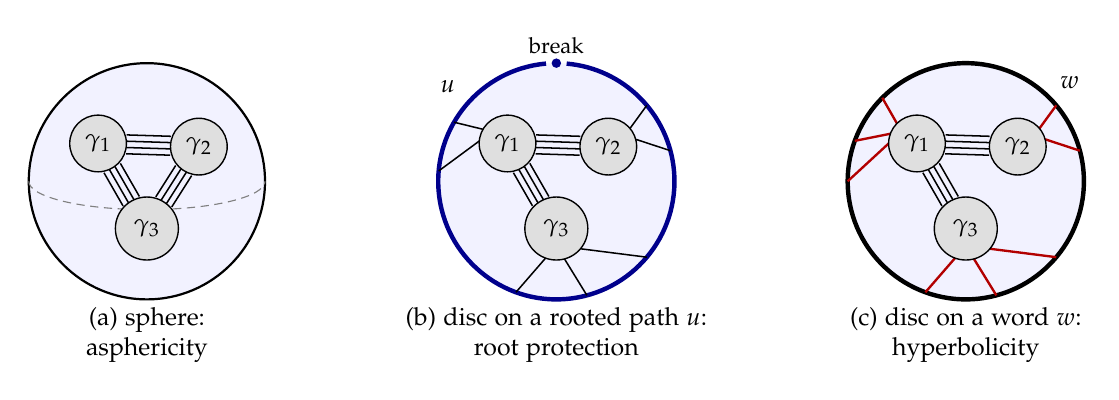
\begin{tikzpicture}[every node/.style={font=\small},
  cone/.style={fill=gray!25,draw=black,line width=0.5pt},
  pair/.style={line width=0.55pt},
  contact/.style={line width=0.85pt,red!70!black}]
\newcommand{\bundle}[4]{\foreach \t in {-0.12,-0.04,0.04,0.12}{
   \draw[pair] ($($(#1)!#3!(#2)$)+($(#1)!\t cm!90:(#2)$)-(#1)$) --
               ($($(#2)!#4!(#1)$)+($(#1)!\t cm!90:(#2)$)-(#1)$);}}
\newcommand{\cones}{
  \draw[cone] (A) circle (0.36); \node at (A) {$\gamma_1$};
  \draw[cone] (B) circle (0.36); \node at (B) {$\gamma_2$};
  \draw[cone] (C) circle (0.4);  \node at (C) {$\gamma_3$};}
\begin{scope}
  \fill[blue!5] (0,0) circle (1.5);
  \draw[line width=0.8pt] (0,0) circle (1.5);
  \draw[densely dashed,gray] (-1.5,0) arc (180:360:1.5 and 0.36);
  \coordinate (A) at (-0.62,0.48); \coordinate (B) at (0.66,0.44); \coordinate (C) at (0,-0.6);
  \bundle{A}{B}{0.36cm}{0.36cm} \bundle{A}{C}{0.36cm}{0.4cm} \bundle{B}{C}{0.36cm}{0.4cm}
  \cones
  \node[align=center] at (0,-1.95) {(a) sphere:\\ asphericity};
\end{scope}
\begin{scope}[xshift=5.2cm]
  \fill[blue!5] (0,0) circle (1.5);
  \draw[line width=1.6pt,blue!55!black] (95:1.5) arc (95:445:1.5);
  \fill[blue!55!black] (90:1.5) circle (0.06);
  \node[above] at (90:1.5) {\footnotesize break};
  \node at (-1.38,1.2) {$u$};
  \coordinate (A) at (-0.62,0.48); \coordinate (B) at (0.66,0.44); \coordinate (C) at (0,-0.6);
  \bundle{A}{B}{0.36cm}{0.36cm} \bundle{A}{C}{0.36cm}{0.4cm}
  \foreach \ang in {150,175} \draw[pair] ($(A)+(\ang:0.36)$) -- (\ang:1.5);
  \foreach \ang in {15,40}   \draw[pair] ($(B)+(\ang:0.36)$) -- (\ang:1.5);
  \foreach \ang in {250,285,320} \draw[pair] ($(C)+(\ang:0.4)$) -- (\ang:1.5);
  \cones
  \node[align=center] at (0,-1.95) {(b) disc on a rooted path $u$:\\ root protection};
\end{scope}
\begin{scope}[xshift=10.4cm]
  \fill[blue!5] (0,0) circle (1.5);
  \draw[line width=1.6pt] (0,0) circle (1.5);
  \node at (1.32,1.25) {$w$};
  \coordinate (A) at (-0.62,0.48); \coordinate (B) at (0.66,0.44); \coordinate (C) at (0,-0.6);
  \bundle{A}{B}{0.36cm}{0.36cm} \bundle{A}{C}{0.36cm}{0.4cm}
  \foreach \ang in {135,160,180} \draw[contact] ($(A)+(\ang:0.36)$) -- (\ang:1.5);
  \foreach \ang in {15,40}       \draw[contact] ($(B)+(\ang:0.36)$) -- (\ang:1.5);
  \foreach \ang in {250,285,320} \draw[contact] ($(C)+(\ang:0.4)$) -- (\ang:1.5);
  \cones
  \node[align=center] at (0,-1.95) {(c) disc on a word $w$:\\ hyperbolicity};
\end{scope}
\end{tikzpicture}
\caption{One estimate, three pictures. Cone disks are bounded by closed paths $\gamma_i$ in $\Gamma$; arcs pair inverse letters. (a) A reduced sphere: every cone letter is paired with a cone letter. (b) A disc bounded by a path $u$ in $\Gamma$ from a root: $u$ is one more path in $\Gamma$, and its letters are counted like the others. (c) A van Kampen disc for a word $w$: the letters of $w$ are discarded, so at most $|w|$ cone letters (red) become unpaired. \Cref{prop:key} excludes (a) and (b) and, for a minimal (c), gives $|w|\ge\frac{13}{16}\eps\sum_i|\gamma_i|\ge\frac{13}{16}\eps\Area(w)$.}
\label{fig:idea}
\end{figure}

\paragraph{Where $a$ comes from.} OpenAI's certificate~\cite[Prop.~2.1]{OAI197a} is a parity count (\cref{prop:parity}). Write $\Gamma=\Gamma_A\sqcup\Gamma_B$, fix roots $x_A\in\Gamma_A$ and $x_B\in\Gamma_B$, and let $A'$ and $B'$ be the vertex sets of their components. For $x\in A'$ let $g_x\in G$ be the label of any path from $x_A$ to $x$, and for $y\in B'$ let $h_y$ be the label of any path from $x_B$ to $y$; these are well defined because the cones kill all closed paths. Put
\[
a=\sum_{x\in A'}g_x,\qquad a^*=\sum_{x\in A'}g_x^{-1},\qquad c=\sum_{y\in B'}h_y^{-1}.
\]
The coefficient of $g$ in $aa^*$ is the parity of the number of pairs $(x,x')$ with $g_xg_{x'}^{-1}=g$. If $x$ and $x'$ both have an outgoing edge labelled $t$, the simultaneous step $(x,x')\mapsto(x\cdot t,x'\cdot t)$ does not change $g_xg_{x'}^{-1}$. OpenAI choose the sets $S_x$ of outgoing labels so that $|S_x\cap S_{x'}|$ is odd for all $(x,x')\neq(x_A,x_A)$, $|S_{x_A}|$ is even, and $|S_x\cap S_y|$ is odd for $x\in A'$, $y\in B'$. By the handshake lemma, every component of the graph of simultaneous steps on $A'\times A'$ has an even number of vertices, except the one containing $(x_A,x_A)$; over $\F_2$ this gives $aa^*=1$, and the same argument on $A'\times B'$ gives $ac=0$. The hard part is to show that $c\neq0$, which holds if no path from $x_B$ to another vertex has trivial label, and that $G$ is torsion-free. Both follow from the exclusions of \cref{fig:idea}(a),(b). Then $a^*a\neq1$, since otherwise $c=a^*(ac)=0$.

\paragraph{A deterministic criterion.} Randomness enters the topology only through one deterministic property of $\Gamma$. Call a finite immersed labelled graph with distinguished roots \emph{pattern-free} (\cref{def:patternfree}) if its vertices have degree at least $5$, its girth is at least $L\ge3$, its components have diameter at most $dL$, it has at most $2^{\lambda L}$ vertices, and it carries no bounded nearly-paired path system: none with at most $K_0$ paths of total length $H\in[L,CL]$, paired by at most $I$ interval pairs with at most $\eps H$ letters unpaired, where $K_0,C,I$ are explicit functions~\eqref{eq:constants} of $\eps,d,\lambda$.

\begin{theorem}\label{thm:C}
If $\Gamma$ is $(\eps,d,\lambda)$-pattern-free at some scale $L$, then the complex $X$ is aspherical, no path in $\Gamma$ from a root to a different vertex has trivial label in $G=\pi_1(X)$, and every word $w$ that is trivial in $G$ satisfies $\Area(w)\le\frac{16}{13\eps}|w|$.
\end{theorem}

\noindent The first two conclusions are OpenAI's argument~\cite[Prop.~4.5 and \S5]{OAI196}, \cite[Thm.~5.2 and \S6]{OAI197a}, run for a fixed graph; the isoperimetric inequality is new. OpenAI's random graphs are pattern-free with probability $1-o(1)$ (\cref{lem:event}), and so are the two random graphs we build for odd $p$ (\cref{cor:zdpatternfree,cor:dfpatternfree}). An explicit pattern-free graph with suitable types would give an explicit example (\cref{sec:remarks}).

\paragraph{Odd characteristic.} By \cref{thm:C}, building counterexamples reduces to building pattern-free graphs with suitable vertex types. OpenAI's certificates need characteristic two. For odd $p$, finitely presented torsion-free groups with a finite two-dimensional classifying space whose group algebras over $\F_p$ have zero divisors were found first by S.~V. Ivanov~\cite[Thm.~1.1]{Ivanov2026}, and independently by us, by the same signed mechanism; Ivanov has precedence. The mechanism signs OpenAI's parity count on a bipartite random model~\cite[Lemma~2.2, Construction~4.1]{Ivanov2026}. If $\Gamma_A$ is bipartite, $\sigma$ is the bipartition sign, $\alpha=\sum_{x\in A'}\sigma(x)g_x$ and $\beta=\sum_{y\in B'}h_y^{-1}$, then a simultaneous step reverses the sign while keeping $g_xh_y^{-1}$ fixed. Pairing each step with its reverse therefore cancels $\sum_{x,y}|S_x\cap S_y|\,\sigma(x)\,g_xh_y^{-1}$ over $\Z$, and this sum is $\alpha\beta$ in $\F_p[G]$ when every such $|S_x\cap S_y|$ is $1$ modulo $p$ (\cref{lem:handshake}). Lines of the projective plane $\PG(2,q)$ over $\F_q$, $q=p^k$, do this, since two of them meet in $1$ or $q+1\equiv1$ points; Ivanov takes $q=p^3$ with $p$ extra letters, the same design on both sides~\cite[Constructions~3.1 and~3.2]{Ivanov2026}. The same sign rule appears earlier, for product structures, as Mineyev's signature condition~\cite[\S2.2]{Mineyev2024} (\cref{sec:remarks}). In hyperbolic groups, zero divisors in odd characteristic are subsumed by \cref{thm:E} below, since a failure of direct finiteness gives idempotents, then zero divisors, then units (\cref{sec:algebra}). The model of \cref{sec:zdodd}, whose types follow OpenAI's asymmetric design (lines of $\PG(2,q)$ and $2p-1$ extra letters), adds only that groups built with the signed zero-divisor mechanism are hyperbolic (\cref{thm:D}); \cref{thm:C} applies in the same way to Ivanov's own model, given his estimates (\cref{rem:ivanovhyp}). \Cref{sec:dfodd} builds on that section.

Direct finiteness, the centre of the odd-characteristic part, needs more. OpenAI's witnesses come from one graph paired with itself and with a second graph, with a single exception at a root~\cite[Prop.~2.1]{OAI197a}. We use the signed cancellation and the two-colour matchings, and pair the root component with itself. In the signed version, $a=\sum_x\sigma(x)g_x$ and $b=-\sum_xg_x^{-1}$, and the types make $|S_x\cap S_{x'}|\equiv1\pmod p$ for all $x,x'$ in the root component, except that $|S_r|\equiv2$ at the root $r$. A type is a line of $\PG(2,p^5)$ with the complement of a line of $\PG(2,p)$, or nothing, as its extra part, and the root carries all of $\PG(2,p)$; for $p=2$ these extra parts are OpenAI's. The exception at the root cannot be avoided, and it creates the new difficulty. The bipartite matchings need, for every letter $t$, as many vertices of one colour carrying $t$ as vertices of the other colour carrying $\bar t$. We solve this colour-balance condition exactly, by an integer-lattice argument in which the pairing $t\mapsto\bar t$ is chosen to satisfy a residue condition modulo $p^5$, and we certify the decay estimate with an explicit rational Perron vector.

\begin{tcolorbox}[headline]
\begin{theorem}\label{thm:E}
For every odd prime $p$ there are a finitely presented, torsion-free, word-hyperbolic group $H_p$ with a finite two-dimensional classifying space and elements $a,b,c\in\F_p[H_p]$ with $ab=1$, $ac=0$ and $c\neq0$. Hence $ba\neq1$, and for every field $K$ of characteristic $p$ the group algebra $K[H_p]$ is not directly finite and contains an idempotent other than $0$ and $1$, a zero divisor and a unit of order $p$ that is not of the form $\lambda g$. Moreover, $H_p$ is neither sofic nor surjunctive.
\end{theorem}
\end{tcolorbox}

\noindent \Cref{thm:A} for $p=2$ and \cref{thm:E} for odd $p$ give the Main Theorem. As far as we know, the groups $H_p$ are the first torsion-free groups whose group algebras over a field of odd characteristic are not directly finite. By the implication noted by Bradford and Fournier-Facio~\cite[\S1]{BFF2024}, they are also counterexamples to the idempotent conjecture, and, as far as we know, the first torsion-free ones in odd characteristic: the earlier torsion-free counterexamples in odd characteristic, Ivanov's zero divisors and Murray's units~\cite{Murray2021}, do not by themselves give idempotents. OpenAI's odd-characteristic counterexample to (D) uses a finitely generated group with torsion, over a field of order $p^4$, for one specified prime $p$~\cite[Thm.~1.1]{OAI197d}. Ivanov's odd-characteristic groups have zero divisors, and nothing is claimed there about direct finiteness or idempotents. The signed form of OpenAI's self-pairing of the root component, with its exception at the root, the exact solution of the colour-balance problem and the Perron certificate are new here.

\paragraph{Consequences.} Since their group algebras over a finite field are not directly finite, the groups of \cref{thm:A,thm:E} are not sofic~\cite[Cor.~4.7]{ElekSzabo2004}, as OpenAI note for the group of \cref{thm:A}~\cite[\S1]{OAI197a}, and not surjunctive, by the standard transfer~\cite[\S1]{ElekSzabo2004}, \cite[Prop.~7.2]{OAI197b} (\cref{lem:surj}). Gottschalk's surjunctivity conjecture~\cite{Gottschalk1973} was disproved in~\cite{OAI197b}, see also~\cite{OAI197d}, with groups that have torsion. To our knowledge, the groups of \cref{thm:A,thm:E} are the first word-hyperbolic groups known not to be surjunctive. Non-sofic hyperbolic groups were obtained in October 2026 in our note~\cite{DouglasMghirbi2026} and, independently, by Sandhu and Thom~\cite{SandhuThom2026}, both building on OpenAI's non-residually-finite hyperbolic group~\cite{OAI252}; \cref{thm:A,thm:E} give such groups by a different, purely algebraic certificate.

\paragraph{Characteristic zero.} Over $\Z$ the signed count of a component need not vanish. Ivanov observed that the obvious designs with constant cross-intersections destroy the decay estimate that makes the groups torsion-free, and wrote that he knew no design combining exact constancy with that estimate~\cite[\S8.2]{Ivanov2026}. \Cref{sec:charzero} proves that none exists: no variant with the cancellation built into the vertex types can work under that estimate. Such cancellation requires the incidence matrices $X_A,X_B$ of the types to satisfy $X_AX_B^{\mathsf T}=\lambda J$, so the sum of their ranks is at most the number $N$ of letters plus one. Over $\F_p$ this is possible because the point--line incidence matrix of a projective plane over a field of characteristic $p$ satisfies $XX^{\mathsf T}=qI+J\equiv J$. Over $\R$, the decay estimate forces each rank above $N/2$ (\cref{thm:rank}).

\paragraph{The example with torsion.} OpenAI's first counterexample to (D)~\cite{OAI197b} uses a group with elements of odd prime order $\ell$, built by gluing copies of $\F_\ell^2$ along their lines according to an incidence structure of girth at least $12$, followed by an HNN extension over finite subgroups and a direct product with a finite group. A link computation, which OpenAI's reasoning trace for~\cite{OAI197b} records together with the possibility of a hyperbolic example at girth $14$~\cite[\S\S12, 17 and~21]{OAItrace}, shows (\cref{sec:cat0}):

\begin{theorem}\label{thm:F}
The group of~\cite[Thm.~1.1]{OAI197b}, whose group algebra over a finite field of characteristic two is not directly finite, acts properly and cocompactly by isometries on a CAT(0) space. If the incidence structure used to build it has girth at least $14$, the group is word-hyperbolic.
\end{theorem}

\paragraph{What is due to whom.} OpenAI's~\cite{OAI196,OAI197a}: the groups and elements of \cref{thm:A,thm:B,cor:zd}; the parity certificates; the random models, the vertex types built from a projective plane and extra letters, and the girth, diameter and bounded-pattern estimates, whose proofs \cref{sec:zdodd,sec:dfodd} rerun; the closure, interval and separation lemmas; and the cone pictures, the surgeries and the exclusion of reduced spheres and rooted discs. Also OpenAI's are the accounting that turns such an exclusion into a linear isoperimetric inequality, for a different random complex~\cite[Thm.~3.1]{OAI257}, and the developability route through the link computation behind \cref{thm:F}, with the possibility of a hyperbolic example at girth $14$, in their reasoning trace~\cite[\S\S12, 17 and~21]{OAItrace}. In priority, Ivanov's~\cite{Ivanov2026}: the first torsion-free zero divisors in odd characteristic, the signed cancellation, the two-colour model, the transfer of OpenAI's estimates to that model with the colour data in the pattern count, and a decay estimate for an odd-characteristic projective-plane design certified by an explicit test vector; the same sign rule appears earlier as Mineyev's signature condition~\cite[\S2.2]{Mineyev2024}. New here: hyperbolicity throughout (the free case of \cref{prop:key}, \cref{thm:C,thm:B} and their consequences); the direct-finiteness construction in odd characteristic, \cref{thm:E}; the characteristic-zero obstruction, \cref{thm:rank}; and a written proof of \cref{thm:F}. \Cref{sec:attribution} gives a sentence-level account, including formal verification and how the work was done.

\paragraph{Organization.} \Cref{sec:algebra} proves the algebra. \Cref{sec:setup} defines pattern-free graphs, states the four inputs (\cref{tab:dictionary}) and proves the deterministic tools. \Cref{sec:key} proves \cref{prop:key} and \cref{thm:C,thm:B}, and \cref{sec:proofA} treats characteristic two (\cref{thm:A,cor:zd,cor:lean}). \Cref{sec:zdodd} sets up the two-colour model and proves \cref{thm:D}, \cref{sec:dfodd} proves \cref{thm:E}, and \cref{sec:charzero} explains why the mechanism stops short of characteristic zero. \Cref{sec:cat0} proves \cref{thm:F}, \cref{sec:remarks} discusses related work and questions, and \cref{sec:attribution} records contributions and how the work was done. \Cref{app:interval} proves the interval lemma, and \cref{app:checks} lists the verification scripts.


\section{The algebra of Kaplansky's conjectures}\label{sec:algebra}

Everything in this section is classical; we include the short proofs because they make the consequences stated in the Main Theorem self-evident. Rings are associative and unital, not necessarily commutative.

\begin{lemma}[one-sided inverses]\label{lem:onesided}
Let $a,b$ be elements of a ring with $ab=1\neq ba$, and put $e=ba$ and $\nu=b(1-e)$. Then $e^2=e\notin\{0,1\}$, $e(1-e)=0=(1-e)e$, and $\nu\neq0=\nu^2$; hence $(1+\nu)(1-\nu)=1=(1-\nu)(1+\nu)$.
\end{lemma}

\begin{proof}
We have $e^2=b(ab)a=e$ and $(1-e)b=b-b(ab)=0$. Hence $e(1-e)=0=(1-e)e$, $\nu^2=b\,[(1-e)b]\,(1-e)=0$, and $(1\pm\nu)(1\mp\nu)=1-\nu^2=1$. Finally, $e\neq1$ by hypothesis, $aeb=(ab)^2=1$ gives $e\neq0$, and $a\nu=1-e\neq0$ gives $\nu\neq0$.
\end{proof}

\begin{lemma}[square-zero elements give non-trivial units]\label{lem:unit}
Let $G$ be torsion-free, $K$ a field, and $\nu\in K[G]$ with $\nu\neq0=\nu^2$. Then $1+\nu$ is a unit of $K[G]$ that is not of the form $\lambda g$.
\end{lemma}

\begin{proof}
Its inverse is $1-\nu$. Suppose that $1+\nu=\lambda g$. If $g=1$, then $\nu$ is a scalar with $\nu^2=0$, so $\nu=0$. If $g\neq1$, then $1,g,g^2$ are distinct because $G$ is torsion-free, so $\nu^2=\lambda^2g^2-2\lambda g+1$ has coefficient $1$ at the identity (also in characteristic two), and $\nu^2\neq0$.
\end{proof}
In characteristic $p>0$, moreover, $(1+\nu)^k=1+k\nu$ for all $k\ge1$, so the unit $1+\nu$ has order exactly $p$.


\begin{lemma}[zero divisors give square-zero elements]\label{lem:connell}
Let $G$ be torsion-free, $K$ a field, and $\alpha,\beta\in K[G]\smallsetminus\{0\}$ with $\alpha\beta=0$. Then $\nu=\beta g\alpha$ satisfies $\nu\neq0=\nu^2$ for some $g\in G$.
\end{lemma}

\begin{proof}
By Connell's theorem, $K[G]$ is a prime ring if and only if $G$ has no non-trivial finite normal subgroup~\cite{Connell1963}, \cite[Thm.~4.2.10]{Passman1977}. So $K[G]$ is prime, hence $\beta K[G]\alpha\neq0$, and since $K[G]$ is spanned by $G$ some $\nu=\beta g\alpha$ is non-zero. Then $\nu^2=\beta g(\alpha\beta)g\alpha=0$.
\end{proof}

For torsion-free $G$, these lemmas give (U)$\Rightarrow$(Z)$\Rightarrow$(I) (an idempotent $e\neq0,1$ satisfies $e(1-e)=0$), and show that a counterexample to (D) is a counterexample to (I), and hence to (Z) and (U); compare~\cite[Ch.~13]{Passman1977}, the introduction of~\cite{Gardam2021}, and~\cite[\S1]{BFF2024}.

\begin{lemma}[direct finiteness, surjunctivity and soficity]\label{lem:surj}
Let $K$ be a finite field and $a,b\in K[G]$ with $ab=1\neq ba$. Then the map $\tau\colon K^G\to K^G$, $\tau(x)=x\ast a$, where $(x\ast a)(g)=\sum_{h}x(gh^{-1})a(h)$, is a cellular automaton over the finite alphabet $K$ that is injective but not surjective. Hence $G$ is neither surjunctive nor sofic.
\end{lemma}

\begin{proof}
The sum is finite and $\tau$ commutes with the left shift, so $\tau$ is a cellular automaton with memory set $(\operatorname{supp}a)^{-1}$. Convolution is associative when the right-hand factors are finitely supported, so $\tau(x)\ast b=x\ast(ab)=x$, and $\tau$ is injective. If $\delta_1=\tau(y)$, then $ba=\delta_1\ast(ba)=(y\ast a)\ast(ba)=y\ast(ab)\ast a=y\ast a=\delta_1$, a contradiction; so $\tau$ is not surjective, and $G$ is not surjunctive~\cite{Gottschalk1973}. Since sofic groups are surjunctive~\cite{Gromov1999,Weiss2000} (and satisfy (D) over every field~\cite[Cor.~4.7]{ElekSzabo2004}), $G$ is not sofic.
\end{proof}

The link between direct finiteness and injective linear cellular automata is classical~\cite{CeccheriniCoornaert2007,Phung2023}.
That a surjunctive group satisfies (D) over finite fields, by exactly this argument, is Elek and Szab\'o's observation~\cite[\S1]{ElekSzabo2004}; OpenAI give a detailed proof of the step from one-sided inverses to cellular automata~\cite[Prop.~7.2]{OAI197b}.

Finally, \emph{base change}: for a field extension $K\subseteq L$, the natural map $K[G]\to L[G]$ is an injective unital ring homomorphism, since $L[G]=L\otimes_KK[G]$ is a free $L$-module with basis $G$. So every identity and every non-identity above that holds over $\F_p$ also holds over every field of characteristic $p$.

\section{Cone complexes, pattern-free graphs and OpenAI's inputs}\label{sec:setup}

\subsection{Labelled graphs, cones and a presentation}
A \emph{signed alphabet} is a finite set $T$ with a fixed-point-free involution $t\mapsto\bar t$; the rose $F$ has one vertex and one edge for each pair $\{t,\bar t\}$, and $\pi_1(F)$ is the free group on $T$ with $\bar t=t^{-1}$. In a $T$-labelled graph $\Gamma$ each oriented edge carries a label, and reversed edges carry inverse labels; $\Gamma$ is \emph{immersed} if the labels of the edges leaving any vertex are distinct, i.e.\ if the label map $\Gamma\to F$ is an immersion. A path is \emph{immersed} if it has no backtracking, and a closed path is \emph{cyclically immersed} if this also holds at its closing turn; in an immersed graph this says exactly that the label is freely, respectively cyclically, reduced. Lengths count edge traversals with multiplicity. The \emph{girth} of $\Gamma$ is the least length of a non-empty cyclically immersed closed path; loops and pairs of parallel edges are cycles of lengths one and two.

For each component $\Lambda$ of $\Gamma$ attach the cone $K_\Lambda$ on $\Lambda$ to $F$ along the label map, obtaining a finite $2$-complex $X$, and put $G=\pi_1(X)$. Choose a spanning tree in each component, and let $R$ be the set of labels of the fundamental cycles of the non-tree edges. Attaching $K_\Lambda$ is homotopy equivalent, relative to $F$, to attaching one $2$-cell along each fundamental cycle~\cite[proof of Lemma~5.2]{OAI196}, so
\begin{equation}\label{eq:presentation}
G=\langle T\mid R\rangle
\end{equation}
is a finite presentation. For a word $w$ that is trivial in $G$, $\Area(w)$ is the least number of conjugates of elements of $R^{\pm1}$ whose product is freely equal to $w$~\cite[Ch.~V]{LyndonSchupp1977}.

\begin{lemma}\label{lem:conearea}
The label of a closed path of length $h$ in a component $\Lambda$ is freely equal to a product of at most $h$ conjugates of elements of $R^{\pm1}$.
\end{lemma}

\begin{proof}
Up to conjugation by the label of a tree path, the closed path is equal, in the fundamental groupoid of $\Lambda$, to the product of the fundamental cycles of the non-tree edges it traverses, in order and with signs; there are at most $h$ of them. Labelling is compatible with free reduction.
\end{proof}

\subsection{Path systems and pattern-free graphs}
Let $\Gamma$ be a finite immersed $T$-labelled graph with a finite set of distinguished vertices, the \emph{roots}.

\begin{definition}[path systems~{\cite[\S3]{OAI196}}]\label{def:system}
A \emph{path system} is a finite family of positive-length paths in $\Gamma$, all closed and cyclically immersed except possibly one immersed interval path that starts at a root. Its \emph{occurrences} are the positions on these paths; distinct occurrences may traverse the same edge. A \emph{pairing by interval pairs} is a family of pairwise disjoint intervals of consecutive occurrences, matched in pairs by order-reversing bijections that match inverse letters, or by order-preserving bijections that match equal letters, subject to the \emph{reduction condition}: matched occurrences traverse distinct undirected edges of $\Gamma$. Occurrences outside the paired intervals are \emph{unpaired}.
\end{definition}

Given $\eps\in(0,1]$ and $d,\lambda\ge1$, put $C_{\rm sep}=2\sqrt2/(1-\sqrt{2/3})$ and, following OpenAI's choices~\cite[Lemma~4.2 and (4.3)]{OAI196}, \cite[Lemma~5.3 and (5.3)]{OAI197a},
\begin{equation}\label{eq:constants}
\begin{gathered}
D_0=\lceil d+4\lambda+8\rceil,\qquad U=\max\{3,\lceil 96D_0/\eps\rceil\},\qquad \eta=\min\Big\{\frac1{32U},\frac{\eps}{64U}\Big\},\\
K_0=\max\{1,\lceil (C_{\rm sep}/\eta)^2\rceil\},\qquad C=K_0(U+D_0),\qquad I=\lceil 192\,C\rceil .
\end{gathered}
\end{equation}
They satisfy
\begin{equation}\label{eq:constineq}
\frac{3D_0}{U}\le\frac{\eps}{32},\qquad 2\eta U\le\frac1{16},\qquad 2\eta U\le\frac{\eps}{32},\qquad \frac{C_{\rm sep}}{\sqrt{K_0}}\le\eta .
\end{equation}

\begin{definition}[pattern-free graphs]\label{def:patternfree}
Let $L\ge3$ be an integer. The rooted graph $\Gamma$ is \emph{$(\eps,d,\lambda)$-pattern-free at scale $L$} if
\begin{enumerate}[label=\textup{(P\arabic*)},itemsep=0pt]
\item every vertex has degree at least $5$, and $\girth(\Gamma)\ge L$;
\item every component of $\Gamma$ has diameter at most $dL$, and $\log_2|V(\Gamma)|\le\lambda L$;
\item $\Gamma$ carries no path system with at most $K_0$ paths and total length $H\in[L,CL]$ with a pairing by at most $I$ interval pairs leaving at most $\eps H$ occurrences unpaired, where $K_0,C,I$ are given by~\eqref{eq:constants}.
\end{enumerate}
\end{definition}

\subsection{OpenAI's random graphs}\label{sec:random}
OpenAI choose $\Gamma=\Gamma_A\sqcup\Gamma_B$ at random~\cite[\S2]{OAI196}, \cite[\S3]{OAI197a}: vertex sets $A$ and $B$ of sizes $n,n$~\cite{OAI196} or $n,n-v$~\cite{OAI197a}, prescribed sets $S_x$ of outgoing labels (``types'') built from the projective plane of order $128$, which has $v=16513$ points~\cite[\S2.1]{OAI196}, and in~\cite[\S3.1]{OAI197a} also from the Fano plane, and independent uniform matchings, conditioned on
\begin{equation}\label{eq:girth}
\girth(\Gamma)\ge L=\lfloor c_0\log n\rfloor
\end{equation}
for a fixed small $c_0>0$. Here $n$ runs through the admissible values: multiples of $2v^2$ in~\cite{OAI196}, and $n=vm$ with $m\equiv1\pmod 4$ in~\cite{OAI197a}. Two roots $x_A\in A$ and $x_B\in B$ are fixed in advance, and $A'$, $B'$ denote the vertex sets of their components. For $x\in A'$ let $g_x\in G$ be the label of any path from $x_A$ to $x$, and for $y\in B'$ let $h_y\in G$ be the label of any path from $x_B$ to $y$; these are well defined because the cones kill the labels of closed paths.

\begin{thm}[OpenAI's inputs~{\cite{OAI196,OAI197a}}]\label{thm:inputs}
In each of the two models there are constants $\eps>0$ and $d\ge1$, depending only on the fixed data of the model, such that:
\begin{enumerate}[label=\textup{(\alph*)},itemsep=0pt]
\item every vertex has degree at least $129$, and the types satisfy the parity hypotheses of \cref{prop:parity}(a) in the model of~\cite{OAI196}, respectively of \cref{prop:parity}(b) in the model of~\cite{OAI197a};
\item for all large admissible $n$ some matching satisfies~\eqref{eq:girth};
\item with probability $1-o(1)$, every component of $\Gamma$ has diameter at most $dL$;
\item \textup{(bounded-pattern estimate)} for every integer $K_0\ge1$, real $C\ge1$ and integer $I\ge0$, with probability $1-o(1)$, $\Gamma$ carries no path system with roots $x_A,x_B$, at most $K_0$ paths and total length $H\in[L,CL]$ with a pairing by at most $I$ interval pairs leaving at most $\eps H$ occurrences unpaired.
\end{enumerate}
Probabilities refer to the girth-conditioned model. \Cref{tab:dictionary} gives the sources.
\end{thm}

The order of quantifiers in (d) is the crux: $\eps$ is fixed before $K_0,C,I$.

\begin{lemma}\label{lem:event}
In either model, let $\eps,d$ be as in \cref{thm:inputs}, $\lambda=1+2/(c_0\log 2)$, and let $E_n$ be the event that $\Gamma$, with roots $x_A,x_B$, is $(\eps,d,\lambda)$-pattern-free at scale $L$. Then $E_n$ has probability $1-o(1)$.
\end{lemma}

\begin{proof}
(P1) holds by \cref{thm:inputs}(a) and~\eqref{eq:girth} once $L\ge3$. For large $n$ we have $L\ge\frac{c_0}{2}\log n$, so $\log_2|V(\Gamma)|\le1+\log_2n\le L+\frac{2}{c_0\log2}L=\lambda L$; with \cref{thm:inputs}(c) this gives (P2) with probability $1-o(1)$. (P3) holds with probability $1-o(1)$ by \cref{thm:inputs}(d) applied to the triple $(K_0,C,I)$ of~\eqref{eq:constants}.
\end{proof}

\begin{table}[!tb]
\centering\footnotesize\setlength{\tabcolsep}{3.5pt}
\begin{tabular}{@{}lllp{3.6cm}ll@{}}
\toprule
Input (\cref{thm:inputs}) & \cite{OAI196} & \cite{OAI197a} & Lean, model of~\cite{OAI196} & \cref{sec:zdodd} & \cref{sec:dfodd} \\
\midrule
(a) types: degrees, parity & \S2.1, (2.1) & \S3.1, Prop.~3.1 & \lean{degreeA/B\_bounds}, \lean{odd\_cross\_inter\-sections} & Lem.~\ref{lem:design} & Lem.~\ref{lem:oddcong} \\
(b) girth $\ge L$ occurs & Lemma 2.2 & \S3.3 & \lean{TypedGraphs.}\allowbreak\lean{eventual\_nonempty} & Lem.~\ref{lem:prescriptions} & Prop.~\ref{prop:oddtransfer}(a) \\
(c) diameter $\le dL$ & Lemma 2.3 & Prop.~3.4 & \lean{diameterA/B\_tendsto} & Lem.~\ref{lem:diameter} & Prop.~\ref{prop:oddtransfer}(b) \\
(d) bounded-pattern estimate & Prop.~3.1 & Thm.~4.1 & \lean{SampleGraph.}\allowbreak\lean{exists\_avoiding}$^{*}$ & Prop.~\ref{prop:patterns} & Prop.~\ref{prop:oddtransfer}(c) \\
\bottomrule
\end{tabular}
\caption{The only inputs from~\cite{OAI196,OAI197a}, and where this paper proves the corresponding inputs for its own models; everything else is proved here. For the models of \cref{sec:zdodd,sec:dfodd}, (a) is the degree bound together with the congruences used by the signed certificates, and (b)--(d) are proved by rerunning OpenAI's proofs. Lean declarations are those of OpenAI's development~\cite{OAIlean}. ${}^{*}$Existence form, with (b) and (c) included and $\eps=1/2467200$: for every fixed triple, some outcome satisfying~\eqref{eq:girth} has the diameter bound and carries no such path system (\cref{cor:lean}).}
\label{tab:dictionary}
\end{table}



\subsection{Three deterministic tools}
The next three lemmas are OpenAI's~\cite[Lemmas~4.2--4.4]{OAI196}, \cite[Lemmas~5.3--5.5]{OAI197a}; we include their short proofs.

\begin{lemma}[short closures]\label{lem:closure}
Let $\Gamma$ satisfy \textup{(P1)} and \textup{(P2)}. Every positive-length immersed path extends to a cyclically immersed closed path by appending at most $D_0L$ edges, without cancelling any of its edges.
\end{lemma}

\begin{proof}
First, for a vertex $z$ and at most two undirected edges at $z$, we find a non-empty immersed closed path at $z$ of length at most $2k$, where $k=\lceil\log_2|V(\Gamma)|\rceil+1$, whose first and last edges avoid the given edges. Delete these edges; since $\girth(\Gamma)\ge3$, every vertex keeps degree at least $3$. There are at least $3\cdot2^{k-1}>|V(\Gamma)|$ non-backtracking walks of length $k$ from $z$, so two distinct ones, $P$ and $Q$, end at the same vertex. Freely reducing $PQ^{-1}$ removes only their common terminal segment; as $P\neq Q$ have the same length, what remains is the required path.

Let $S$ run from $a$ to $b$, and let $R$ be a geodesic from $b$ to $a$, of length at most $dL$. Choose such a closed path $J_b$ at $b$ avoiding the last edge of $S$ and the first edge of $R$, and $J_a$ at $a$ avoiding the last edge of $R$ and the first edge of $S$. Then $SJ_bRJ_a$ has no backtracking at any join, including the closing one; if $R$ is empty, use $SJ_a$ with $J_a$ avoiding the first and last edges of $S$. The added length is at most $dL+4k\le dL+4(\lambda L+2)\le D_0L$.
\end{proof}

\begin{lemma}[recursive planar separation]\label{lem:separator}
For every integer $K_0\ge1$, every planar multigraph with $m$ vertices has a set of at most $C_{\rm sep}m/\sqrt{K_0}$ vertices whose removal leaves components with at most $K_0$ vertices.
\end{lemma}

\begin{proof}
Removing loops and multiple edges changes no components. By Lipton and Tarjan~\cite[Cor.~2]{LiptonTarjan1979}, a simple planar graph with $s$ vertices has at most $2\sqrt2\sqrt s$ vertices whose removal leaves components with at most $2s/3$ vertices. Apply this recursively to every component with more than $K_0$ vertices, charging $2\sqrt2/\sqrt s$ to each of its $s$ vertices; the charges at that step total $2\sqrt2\sqrt s$, which bounds the number of vertices removed. Along the recursion, the components containing a given vertex shrink by factors of at least $3/2$ and have more than $K_0$ vertices, so its total charge is at most $\frac{2\sqrt2}{\sqrt{K_0}}\sum_{j\ge0}(2/3)^{j/2}=C_{\rm sep}/\sqrt{K_0}$.
\end{proof}

\begin{lemma}[interval lemma]\label{lem:interval}
Let $S$ be an oriented sphere containing disjoint closed disks $D_1,\dots,D_{N_0}$. Suppose that each $\partial D_i$, oriented as the boundary of $D_i$, carries a non-empty cyclic word, and that these words are cyclically reduced except that one circle may contain a marked gap between consecutive letters, the \emph{break}, where the two letters may be inverse. Suppose that disjoint arcs in $S\smallsetminus\bigcup_i\operatorname{int}D_i$ join the letter occurrences in pairs, each occurrence lying on exactly one arc and joined occurrences carrying inverse letters. Cut the circles into $N'\ge N_0$ pieces of consecutive occurrences, cutting at the break. Then the arcs are described by at most $6N'$ pairs of intervals, each interval consisting of consecutive occurrences in a single piece and each pair matched in reversed order.
\end{lemma}

The proof (\cref{app:interval}) uses only planarity and the absence of inverse adjacent letters, never that the boundaries are paths in $\Gamma$; this is what allows a boundary reading an arbitrary word.

\section{One estimate, three consequences}\label{sec:key}

Throughout this section $\Gamma$ is $(\eps,d,\lambda)$-pattern-free at scale $L$, and $X$, $G$ are its cone complex and group.

\subsection{Cone pictures}
We use pictures, the dual form of van Kampen diagrams~\cite{vanKampen1933,Rourke1979,CollinsHuebschmann1982,Pride1991,BogleyPride1993}, in the cone version of~\cite[\S5.1]{OAI196}.

\begin{definition}[cone pictures]\label{def:picture}
A \emph{cone picture} consists of an oriented $2$-sphere $S$, disjoint closed disks $D_1,\dots,D_k$ ($k\ge0$), the \emph{cone disks}, at most one further disjoint closed disk $D_\infty$, the \emph{outer disk}, and disjoint arcs in the complement of the disks, such that, reading each boundary circle as the boundary of its own disk, each $\partial D_i$ reads the label of a closed path $\gamma_i$ in $\Gamma$, every letter occurrence on the circles is an endpoint of exactly one arc, and the two occurrences joined by an arc carry inverse letters. The picture is
\begin{itemize}[itemsep=0pt]
\item \emph{spherical} if there is no outer disk;
\item \emph{free} if $\partial D_\infty$ reads a word; it is a \emph{capped picture for $w$} if this word is $w^{-1}$;
\item \emph{rooted} if $\partial D_\infty$ carries a marked point, the \emph{break}, and read from the break reads the label of a path $u$ in $\Gamma$ that starts at a root.
\end{itemize}
The \emph{graph boundaries} are the $\partial D_i$ and, in the rooted case, $\partial D_\infty$; their occurrences traverse edges of $\Gamma$. The \emph{cone length} is $H_0=\sum_i|\gamma_i|$. The picture is \emph{reduced} if
\begin{enumerate}[label=\textup{(R\arabic*)},itemsep=0pt]
\item $k\ge1$, every $\gamma_i$ is non-empty and cyclically immersed, in the free case the outer word is non-empty and cyclically reduced, and in the rooted case $u$ is non-empty and immersed;
\item no arc joins two occurrences on graph boundaries that traverse the same undirected edge of $\Gamma$.
\end{enumerate}
\end{definition}

\begin{lemma}\label{lem:pictures}
\textup{(a)} A non-empty word $w$ is trivial in $G$ if and only if it admits a capped picture, and then $\Area(w)$ is at most the cone length of any capped picture for $w$.
\textup{(b)} A spherical cone picture $P$ defines a map $f_P\colon S\to X$, well defined up to homotopy, and if $\pi_2(X)\neq0$, then $f_P$ is essential for some spherical cone picture $P$.
\end{lemma}

\begin{proof}
(a) Regard the labels of all closed paths in $\Gamma$ as (infinitely many) relators; their normal closure is the kernel of $\pi_1(F)\to G$, and a capped picture is a picture over this presentation in which the boundary reads $w$. If $w$ is trivial, a van Kampen diagram for $w$ over~\eqref{eq:presentation}~\cite[Ch.~V]{LyndonSchupp1977}, placed on a sphere whose complementary face becomes $D_\infty$, is dual to such a picture: each $2$-cell becomes a cone disk bounded by a fundamental cycle, and each edge is crossed by one arc~\cite{Rourke1979,Pride1991}. Conversely, a picture with cone disks $D_1,\dots,D_k$ exhibits $w$ as freely equal to a product of conjugates of the labels of $\gamma_1^{\pm1},\dots,\gamma_k^{\pm1}$~\cite[\S1]{Pride1991}, \cite{BogleyPride1993}; by \cref{lem:conearea} each of these is a product of at most $|\gamma_i|$ conjugates of elements of $R^{\pm1}$, so $\Area(w)\le\sum_i|\gamma_i|$.

(b) Send the complement of the disks and of a neighbourhood of the arcs to the vertex of $F$, a neighbourhood of each arc across the corresponding edge of $F$, and $D_i$ to the cone on $\gamma_i$ in $K_\Lambda$. By the cone version~\cite[Lemma~5.2]{OAI196} of the classical fact for presentation complexes~\cite{Rourke1979}, \cite[\S1]{Pride1991}, \cite{BogleyPride1993}, transported along the homotopy equivalence of~\eqref{eq:presentation}, an essential map $S\to X$ is homotopic to a map that agrees with $f_P$ for some spherical cone picture $P$, except that the preimages of the midpoints of the edges of $F$ may also contain closed curves. A closed curve $c$ maps to one point, so collapsing $c$ writes the class as a sum of translates of the classes of the two spheres obtained from the discs bounded by $c$; one of them is essential, and each has fewer closed curves. Induction on the number of closed curves gives an essential $f_P$.
\end{proof}

\subsection{Minimal pictures are reduced}
We consider three minimization problems.
\begin{enumerate}[itemsep=0pt]
\item[\textup{(S)}] Spherical cone pictures $P$ with $f_P$ essential.
\item[\textup{(F)}] Capped pictures for a fixed non-empty cyclically reduced word $w$ that is trivial in $G$.
\item[\textup{(R)}] Pairs $(u,P)$, where $u$ is a path from a fixed root $r$ to a fixed vertex $y\neq r$ and $P$ is a rooted cone picture whose outer disk reads $u$ from the break.
\end{enumerate}
In each, the complexity is $H_0$, respectively $H_0$, respectively $|u|+H_0$, followed by the number $k$ of cone disks, ordered lexicographically.

\begin{lemma}\label{lem:reduced}
In each of the problems \textup{(S)}, \textup{(F)}, \textup{(R)}, a solution of least complexity is reduced.
\end{lemma}

\begin{proof}
We list moves that apply whenever (R1) or (R2) fails. Each produces a solution of the same problem of smaller complexity, except that in (S) the last move may produce two spherical pictures, one of which is then a solution of smaller complexity. Since each cone $K_\Lambda$ is contractible, two maps of a disc into $K_\Lambda$ that agree on the boundary are homotopic relative to it; this is why the moves other than splitting do not change the class of $f_P$ in (S). Moves in (F) never touch $D_\infty$.

\emph{Empty disks.} A cone disk with $|\gamma_i|=0$ carries no arcs and is deleted.

\emph{Tightening.} Suppose that two consecutive occurrences on a graph boundary read $\sigma\sigma^{-1}$ for an edge $\sigma$ (on $\partial D_\infty$, not across the break). If they are joined to each other, apply splitting below, with $p$, respectively $u_2$, empty. Otherwise shrink the disk to exclude them and join their two arcs, through the excised region, into one arc, which again joins inverse letters. A cone path loses two edges, and in (R) the path $u$ loses two edges and keeps its endpoints.

\emph{Merging.} Suppose an arc $\theta$ joins occurrences on two different graph boundaries that traverse the same undirected edge. Joined occurrences carry inverse letters and $t\mapsto\bar t$ has no fixed points, so they traverse the edge in opposite directions, as $\sigma$ and $\sigma^{-1}$. Thicken $\theta$ to a band. The two disks and the band form one disk, whose boundary reads the path obtained by replacing $\sigma$ in one boundary path by the rest of the other: if $\gamma_i=\sigma p$ and $\gamma_j=\sigma^{-1}q$ cyclically, it reads $pq$; in (R), if $u=u_1\sigma u_2$ and $\gamma_i=\sigma^{-1}q$, it reads $u_1qu_2$, with the same endpoints and break. The band lifts to the edge $\sigma$ of $\Lambda$, so in (S) the new disk still maps into $K_\Lambda$.

\emph{Splitting.} Suppose $\theta$ joins two occurrences of $\sigma$ and $\sigma^{-1}$ on the same graph boundary. The disk and the band form an annulus $A$, crossed by no arc. For a cone disk, write $\gamma_i=\sigma p\sigma^{-1}q$, so the circles of $A$ read the closed paths $p$ and $q$, bounding complementary components $U_p$ and $U_q$. In (F) and (R), delete everything in the component not containing $D_\infty$, and fill it together with $A$ by one cone disk bounded by the other circle. In (S), let $P'$ be obtained by filling $A\cup U_p$ by a cone disk bounded by $q$, and $P''$ by filling $A\cup U_q$ by a cone disk bounded by $p$. Capping the circles of $A$ by cones in $K_\Lambda$ writes $f_P$ as a sum of translates of $f_{P'}$, $f_{P''}$ and a map into $K_\Lambda$; so one of $f_{P'},f_{P''}$ is essential, and both have smaller cone length. For the outer disk in (R), write $u=u_1\sigma u_2\sigma^{-1}u_3$: the circles of $A$ read the closed path $u_2$ and, from the break, $u_1u_3$; delete everything in the component bounded by the $u_2$-circle and let it, with $A$, be the new outer disk.

In every case the complexity drops, by at least two in the length or by one in $k$. So a solution of least complexity admits none of these moves: its cone paths are non-empty and cyclically immersed, in (R) the path $u$ is immersed, and (R2) holds. It remains to show that $k\ge1$. If $k=0$, the arcs form a non-crossing matching of inverse letters on the outer circle, so the outer word is trivial in the free group. In (F) this contradicts cyclic reducedness, and in (R) the label of the non-empty immersed path $u$ is freely reduced, a contradiction. In (S), $f_P$ maps into the graph $F$ and is inessential.
\end{proof}

\subsection{The key estimate}
\begin{proposition}\label{prop:key}
Let $P$ be a reduced cone picture. Then $P$ is not rooted, and
\[
H_0\;\le\;\frac{16}{13\,\eps}\,\ell_\infty ,
\]
where $\ell_\infty$ is the length of the outer word ($\ell_\infty=0$ if $P$ is spherical). In particular, there is no reduced spherical picture.
\end{proposition}

\begin{proof}
Let $H$ be the total length of the graph boundaries: $H=H_0$, plus $|u|$ in the rooted case. Since $k\ge1$, the girth gives $H\ge H_0\ge L$. Suppose that $P$ is rooted, or that $\ell_\infty<\frac{13}{16}\eps H_0$; we derive a contradiction. We follow the proof of~\cite[Prop.~4.5]{OAI196} (equivalently~\cite[Thm.~5.2]{OAI197a}), with a free outer disk as an extra boundary all of whose arcs are discarded.

\emph{Split and close.} Keep each graph boundary path of length at most $UL$. Split a longer one, of length $h$, into $m=\lceil h/UL\rceil$ consecutive segments whose lengths differ by at most one, cutting $u$ along its order from the root; since $UL\ge6$, these lengths lie between $UL/3$ and $UL$. Close each segment to a cyclically immersed closed path by \cref{lem:closure}, and declare the added occurrences unpaired. This gives $k'$ \emph{pieces}: closed cyclically immersed paths with between $L$ and $UL$ original occurrences and of length at most $(U+D_0)L$, and possibly the intact rooted path $u$, if $|u|\le UL$. Since $m\le2h/UL$, the total added length and the number of pieces satisfy
\begin{equation}\label{eq:pieces}
H_{\rm add}\le\frac{2D_0}{U}H,\qquad k'L\le H+L\le 2H .
\end{equation}

\emph{Intervals.} Apply \cref{lem:interval} to $P$, with the graph boundaries cut into the $k'$ pieces (the break being a cut) and a free outer circle as one more piece. In the rooted case there are $k'$ pieces; otherwise every piece has at least $L$ occurrences, so $k'L\le H$, and there is at most one more piece. Either way the arcs are described by at most $12H/L$ interval pairs, each interval lying in one piece. Keep only the pairs both of whose intervals lie on graph pieces; by (R2) they satisfy the reduction condition.

\emph{Separate.} The multigraph whose vertices are the $k'$ graph pieces and whose edges are the arcs between them is planar~\cite[proof of Prop.~4.5]{OAI196}: draw one vertex per piece inside its disk, and omit arcs ending on a free outer disk. By \cref{lem:separator} and~\eqref{eq:constineq}, deleting at most $\eta k'$ pieces leaves components, the \emph{clusters}, of at most $K_0$ pieces each. The deleted pieces contain at most $M_{\rm del}\le\eta k'UL\le2\eta UH$ original occurrences, so at most $M_{\rm del}$ surviving occurrences lose their partner. An interval pair is retained if both of its intervals survive; its two pieces are then adjacent, hence in the same cluster.

\emph{Count.} For a cluster $Z$ let $H_Z$ be its total length (closures included), $b_Z$ its number of unpaired occurrences, and $I_Z$ its number of retained interval pairs. An occurrence of $Z$ is unpaired only if it was added by a closure, its partner was deleted, or its arc ends on a free outer disk; there are at most $\ell_\infty$ of the last kind. By~\eqref{eq:pieces} and~\eqref{eq:constineq},
\[
\sum_Z H_Z\ge(1-2\eta U)H\ge\tfrac{15}{16}H,\qquad
\sum_Z b_Z\le\Big(\frac{2D_0}{U}+2\eta U\Big)H+\ell_\infty\le\frac{\eps}{16}H+\ell_\infty,
\]
and $\sum_Z I_Z\le12H/L$. Call $Z$ \emph{good} if $b_Z\le\eps H_Z$ and $I_Z\le192H_Z/L$. Clusters violating the first condition have total length at most $\eps^{-1}\sum_Zb_Z$, and clusters violating the second have total length at most $\frac{L}{192}\sum_ZI_Z$. Therefore
\begin{equation}\label{eq:chain}
\tfrac{15}{16}H\;\le\;\sum_Z H_Z\;\le\;\underbrace{\tfrac1\eps\textstyle\sum_Z b_Z}_{\le\, H/16\,+\,\ell_\infty/\eps}\;+\;\underbrace{\tfrac{L}{192}\textstyle\sum_Z I_Z}_{\le\, H/16}\;+\;\sum_{Z\ \mathrm{good}}H_Z ,
\end{equation}
so the good clusters have total length at least $\frac{13}{16}H-\ell_\infty/\eps$.

\emph{Contradiction.} If $P$ is not rooted, then $H=H_0$, this is positive by assumption, and every cluster has length at least $L$. If $P$ is rooted, then $\ell_\infty=0$; a cluster shorter than $L$ consists of the intact path $u$ alone, of length $h<L$, and since some cone disk is disjoint from it, $H\ge h+L>2h$. Discarding that cluster leaves good clusters of total length at least $(\frac{13}{16}-\frac12)H>0$. In both cases there is a good cluster $Z$ with $H_Z\ge L$. It consists of at most $K_0$ paths, closed and cyclically immersed except possibly the rooted path $u$, so $L\le H_Z\le K_0(U+D_0)L=CL$; it has $b_Z\le\eps H_Z$ and $I_Z\le192H_Z/L\le192C\le I$; and its retained pairs form a pairing by interval pairs satisfying the reduction condition. This contradicts (P3).
\end{proof}

\begin{remark}\label{rem:diff}
\Cref{prop:key} is OpenAI's exclusion argument~\cite[Prop.~4.5]{OAI196}, \cite[Thm.~5.2]{OAI197a} with one new case. A free outer disk differs from OpenAI's boundaries in three ways: it is not a path in $\Gamma$, which is harmless because its arcs are discarded and the interval lemma needs only cyclic reducedness; its at most $\ell_\infty$ arcs add at most $\ell_\infty$ unpaired occurrences, the source of the term $\ell_\infty/\eps$ in~\eqref{eq:chain}; and no surgery touches it. No union bound over the size of the picture is used: the same fixed triple $(K_0,C,I)$ handles every sphere, every rooted disc and every word. The same accounting, with contacts on the outer boundary paid for by its length, gives a linear isoperimetric inequality for a different random complex in~\cite[Thm.~3.1 and Lemma~3.8]{OAI257}.
\end{remark}

\subsection{Asphericity, root protection and hyperbolicity}

\begin{proof}[Proof of \cref{thm:C}]
\emph{Asphericity.} If $\pi_2(X)\neq0$, \cref{lem:pictures}(b) gives a spherical cone picture $P$ with $f_P$ essential; by \cref{lem:reduced} one of least complexity is reduced, contradicting \cref{prop:key}. So $\pi_2(X)=0$. The universal cover of $X$ is a simply connected $2$-complex with $H_2\cong\pi_2(X)=0$, hence contractible~\cite[Thm.~4.32, Cor.~4.33]{Hatcher2002}. Thus $X$ is a finite two-dimensional $K(G,1)$, and $G$, having a finite-dimensional classifying space, is torsion-free~\cite[\S VIII.2]{Brown1982}.

\emph{Roots.} Suppose that a path $u$ from a root $r$ to a vertex $y\neq r$ has trivial label; $u$ is non-empty. By \cref{lem:pictures}(a), the word $w$ with $w^{-1}=\operatorname{label}(u)$ has a capped picture; marking a break between the last and first letters of $\partial D_\infty$ makes it a rooted picture for $u$. By \cref{lem:reduced}, a pair of least complexity in problem (R) is reduced, contradicting \cref{prop:key}.

\emph{Isoperimetry.} Free reduction and cyclic permutation do not increase length, and conjugation does not change area, so it suffices to take $w$ non-empty and cyclically reduced. By \cref{lem:pictures}(a) and \cref{lem:reduced}, a capped picture for $w$ of least complexity is reduced, and by \cref{lem:pictures}(a) and \cref{prop:key}, $\Area(w)\le H_0\le\frac{16}{13\eps}|w|$.
\end{proof}

\begin{proof}[Proof of \cref{thm:B}]
On the event $E_n$ of \cref{lem:event}, $\Gamma$ is pattern-free, so \cref{thm:C} gives the isoperimetric inequality. A finitely presented group with a linear Dehn function is word-hyperbolic. This is Gromov's theorem~\cite[2.3.D, proved in 6.8]{Gromov1987}; complete proofs are given in~\cite[Thm.~2.5]{ABCFLMSS1991}, \cite{Olshanskii1991} and~\cite[Thm.~III.H.2.9]{BridsonHaefliger1999}, and see~\cite[Thm.~6.1.5]{Bridson2002}.
\end{proof}
\section{Characteristic two}\label{sec:proofA}

\begin{proposition}[OpenAI's parity certificates~{\cite[\S6]{OAI196}, \cite[Prop.~2.1]{OAI197a}}]\label{prop:parity}
Let $\Gamma=\Gamma_A\sqcup\Gamma_B$ be a finite immersed labelled graph without loops, with roots $x_A,x_B$, notation as in \cref{sec:random}, and let $S_x$ be the set of labels of the edges leaving $x$. Put $a=\sum_{x\in A'}g_x$ and $c=\sum_{y\in B'}h_y^{-1}$ in $\F_2[G]$.
\begin{enumerate}[label=\textup{(\alph*)},itemsep=0pt]
\item If $|S_x\cap S_y|$ is odd for all $x\in A'$ and $y\in B'$, then $ac=0$.
\item If moreover $|S_x\cap S_{x'}|$ is odd for all $(x,x')\in A'\times A'$ other than $(x_A,x_A)$, and $|S_{x_A}|$ is even, then $aa^*=1$.
\item If no path from $x_A$, respectively $x_B$, to a different vertex has trivial label, then $a\neq0$, respectively $c\neq0$; in case \textup{(b)} then $a^*a\neq1$.
\end{enumerate}
\end{proposition}

\begin{proof}
For $x\in A'$ and $t\in S_x$ let $x\cdot t$ be the end of the edge labelled $t$ at $x$, so that $g_{x\cdot t}=g_xt$. On $A'\times B'$, join $(x,y)$ to $(x\cdot t,y\cdot t)$ for every $t\in S_x\cap S_y$; the step labelled $\bar t$ at the endpoint is the same edge reversed. This multigraph has no loops, the vertex $(x,y)$ has degree $|S_x\cap S_y|$, and $g_xh_y^{-1}$ is constant on each component, since $(g_xt)(h_yt)^{-1}=g_xh_y^{-1}$. By the handshake lemma, a component in which every degree is odd has an even number of vertices. The coefficient of $g$ in $ac=\sum_{x,y}g_xh_y^{-1}$ is the number of vertices with value $g$, a sum of sizes of components, hence even: (a). In (b), the same multigraph on $A'\times A'$, with values $g_xg_{x'}^{-1}$, has odd degrees except at $(x_A,x_A)$, whose component therefore has odd size and value $1$; all other components have even size, so $aa^*=\sum_{x,x'}g_xg_{x'}^{-1}=1$. In (c), only $x_A$ contributes $1$ to $a$, and only $x_B$ to $c$, so their coefficients of $1$ are $1$. Finally, if $a^*a=1$ then $c=a^*(ac)=0$.
\end{proof}

\begin{corollary}[the case $p=2$; $G$ and $a$ from~{\cite[Thm.~1.1 and Prop.~2.1]{OAI197a}}]\label{thm:A}
There are a finitely presented, torsion-free, word-hyperbolic group $G$ with a finite two-dimensional classifying space and an element $a\in\F_2[G]$ with $aa^*=1\neq a^*a$. Consequently, with $e=a^*a$ and $\nu=a^*(1-e)$:
\begin{enumerate}[label=\textup{(\roman*)},itemsep=0pt,topsep=2pt]
\item $e$ is an idempotent different from $0$ and $1$, so \textup{(I)} and \textup{(D)} fail;
\item $e(1-e)=0$ with $e\neq0\neq1-e$, so \textup{(Z)} fails;
\item $\nu\neq0=\nu^2$, so $1+\nu$ is a unit of order two that is not of the form $\lambda g$, so \textup{(U)} fails.
\end{enumerate}
Moreover, $G$ is neither sofic nor surjunctive.
\end{corollary}

\begin{proof}[Proof of \cref{thm:A}]
Work in the model of~\cite{OAI197a}, choose $n$ large and $\Gamma\in E_n$ (\cref{lem:event}), and let $G=\pi_1(X)$. By \cref{thm:C}, $X$ is a finite aspherical $2$-complex, so $G$ is finitely presented, torsion-free and has a finite two-dimensional classifying space; its roots are protected; and $G$ is word-hyperbolic. $\Gamma$ has no loops, and by \cref{thm:inputs}(a) its types satisfy the hypotheses of \cref{prop:parity}(b), so $aa^*=1\neq a^*a$. Items (i)--(iii) follow from \cref{lem:onesided} with $b=a^*$ and \cref{lem:unit}, and $(1+\nu)^2=1+\nu^2=1$ in characteristic two. \Cref{lem:surj} shows that $G$ is neither sofic nor surjunctive.
\end{proof}

\begin{corollary}\label{cor:zd}
In the model of~\cite{OAI196}, for every large admissible $n$ and every $\Gamma\in E_n$, the group $G$ is finitely presented, torsion-free and word-hyperbolic, with a finite two-dimensional classifying space, and $\alpha=\sum_{x\in A'}g_x$ and $\beta=\sum_{y\in B'}h_y^{-1}$ are non-zero elements of $\F_2[G]$ with $\alpha\beta=0$. Hence $\F_2[G]$ contains a non-trivial unit.
\end{corollary}

\begin{proof}
As for \cref{thm:A}, using \cref{prop:parity}(a),(c), whose hypothesis holds by \cref{thm:inputs}(a), and then \cref{lem:connell,lem:unit}.
\end{proof}

\begin{corollary}\label{cor:lean}
In the model of~\cite{OAI196} as formalized by OpenAI~\cite{OAIlean}, for all large $n$ there is an outcome $\Gamma$ satisfying the conclusions of \cref{cor:zd} for which, with respect to~\eqref{eq:presentation},
\[
\Area(w)\le 3{,}036{,}554\,|w|\qquad\text{for every word $w$ that is trivial in $G$}.
\]
The only inputs from OpenAI used in the proof, \cref{thm:inputs}\textup{(a)--(d)} in the existence form below, are formalized in Lean.
\end{corollary}

\begin{proof}
OpenAI's Lean development proves the following existence form of \cref{thm:inputs}(b)--(d), as \lean{SampleGraph.exists\_avoiding}: there are explicit constants $\eps_*=1/2467200$ and $d_*$ such that for all natural numbers $C,K_0,I'\ge1$, all large $n$ and all roots $x_A,x_B$, some matching satisfies~\eqref{eq:girth}, has all component diameters at most $d_*L$, and carries no path system with at most $K_0$ paths and total length in $[L,CL]$ with at most $I'$ interval sides, that is $\lfloor I'/2\rfloor$ interval pairs, leaving at most $\eps_*H$ occurrences unpaired. There $n=2v^2m$ and $L=\lfloor(\log n)/100\rfloor$, intervals are linear in a fixed indexing of each path (we index each closed piece from one of its cuts), \lean{degreeA\_bounds} and \lean{degreeB\_bounds} give degrees in $[129,132]$, and \lean{odd\_cross\_intersections} gives the parity hypothesis of \cref{prop:parity}(a). Take $\eps=\eps_*$, $d=d_*$ and $\lambda=1+200/\log2$, compute $K_0,C,I$ by~\eqref{eq:constants}, and apply this with $I'=2I$. The resulting $\Gamma$ is pattern-free, as in the proof of \cref{lem:event}. \Cref{thm:C} and \cref{prop:parity} give the conclusions, with $\frac{16}{13\eps_*}=\frac{39475200}{13}<3{,}036{,}554$.
\end{proof}

\Cref{cor:lean} is weaker than \cref{thm:A}, which also needs~\cite{OAI197a}, but its OpenAI inputs are formalized in Lean, as reported by OpenAI; we have not rebuilt the development. \Cref{sec:attribution} states exactly what this means.

\section{The two-colour model: zero divisors in odd characteristic}\label{sec:zdodd}

Fix an odd prime $p$. In hyperbolic groups, zero divisors over $\F_p$ are subsumed by \cref{thm:E}: a failure of direct finiteness gives idempotents, then zero divisors, then units (\cref{sec:algebra}). Without hyperbolicity, torsion-free zero divisors in odd characteristic are Ivanov's theorem~\cite[Thm.~1.1]{Ivanov2026}. This section sets up what \cref{sec:dfodd,sec:charzero} build on: the signed cancellation, a type design that follows OpenAI's asymmetric types, the two-colour model, its squared-word decay and the colour data in the pattern count. Its only further content is \cref{thm:D}: groups built with the signed zero-divisor mechanism are hyperbolic.

\subsection{Signed cancellation}
We use the notation of \cref{sec:setup,prop:parity}: $S_x$ is the set of labels of the edges leaving a vertex $x$, and $x\cdot t$ is the end of the edge labelled $t$ at $x$.

\begin{lemma}[signed cancellation~{\cite[Lemma~2.2]{Ivanov2026}}]\label{lem:handshake}
Let $A'$ and $B'$ be the vertex sets of components, possibly the same one, of finite immersed graphs labelled over the same signed alphabet, with path labels $g_x$ $(x\in A')$ and $h_y$ $(y\in B')$ in a group $G$, so that $g_{x\cdot t}=g_xt$ and $h_{y\cdot t}=h_yt$. Let $\sigma\colon A'\to\{\pm1\}$ satisfy $\sigma(x\cdot t)=-\sigma(x)$ for all $x\in A'$ and $t\in S_x$.
\begin{enumerate}[label=\textup{(\alph*)},itemsep=0pt]
\item In $\Z[G]$,
\begin{equation}\label{eq:handshake}
\sum_{x\in A',\,y\in B'}|S_x\cap S_y|\,\sigma(x)\,g_xh_y^{-1}=0 .
\end{equation}
\item If $R$ is a commutative ring in which $|S_x\cap S_y|\cdot1_R=1_R$ for all $x\in A'$ and $y\in B'$, then
\[
\Bigl(\sum_{x\in A'}\sigma(x)\,g_x\Bigr)\Bigl(\sum_{y\in B'}h_y^{-1}\Bigr)=0\qquad\text{in }R[G].
\]
\item For any map $\sigma\colon A'\to\{\pm1\}$, alternating or not: if no path from a vertex $x_A\in A'$ to a different vertex has trivial label, then the coefficient of $1$ in $\sum_{x\in A'}\sigma(x)g_x$ is $\sigma(x_A)$; in particular this sum is non-zero.
\end{enumerate}
\end{lemma}

\begin{proof}
(a) Let $\Phi=\{(x,y,t):x\in A',\,y\in B',\,t\in S_x\cap S_y\}$ and $\iota(x,y,t)=(x\cdot t,\,y\cdot t,\,\bar t)$. Since $\bar t\in S_{x\cdot t}\cap S_{y\cdot t}$ and $(x\cdot t)\cdot\bar t=x$, the map $\iota$ is an involution of $\Phi$, and it has no fixed points because $\bar t\neq t$. Put $\omega(x,y,t)=\sigma(x)\,g_xh_y^{-1}$. Then
\[
\omega(\iota(x,y,t))=\sigma(x\cdot t)\,g_xt\,(h_yt)^{-1}=-\omega(x,y,t),
\]
so the $\iota$-orbits cancel in pairs and $\sum_\Phi\omega=0$. Grouping $\Phi$ by $(x,y)$ gives the left side of~\eqref{eq:handshake}. (b) Map~\eqref{eq:handshake} to $R[G]$; by the hypothesis on $R$ its left side becomes the product. (c) The only vertex with $g_x=1$ is $x_A$.
\end{proof}

Parts~(a) and~(b) are~\cite[Lemma~2.2]{Ivanov2026}, which allows any common residue $d\not\equiv0$ in place of $1$; part~(a) is the identity over $\Z$ of Step~3 of his proof, stated here for possibly equal components, which \cref{sec:dfodd} needs. Part~(c) is noted there too. The lemma is OpenAI's parity argument (\cref{prop:parity}) with a sign. The same sign rule appears earlier as Mineyev's signature condition~\cite[\S2.2]{Mineyev2024}, with $\sigma\equiv1$ on $B'$, for the pairs $\{(x,y,t),\iota(x,y,t)\}$; \cref{sec:remarks} explains how the two differ. In characteristic two the sign is invisible, and the hypothesis of~(b) reads ``every $|S_x\cap S_y|$ is odd''. Two features are essential. First, bipartiteness: without the sign reversal the orbit sums do not cancel. Second, the hypothesis is only a congruence. Over $\Z$ the signed vertex count of a single component of the simultaneous-step graph need not vanish, and \cref{sec:charzero} shows that this cannot be repaired by cancellation built into the vertex types under the same decay estimate.

\subsection{Vertex types in characteristic \texorpdfstring{$p$}{p}}

Put $e=2p-1$ and choose a power $q=p^k$ with $q\ge 2e(e+2)$; for $p=3$ we take $q=81$. Let $v=q^2+q+1$ and $\lambda=(q+1)/v$, the proportion of lines of $\PG(2,q)$ through a given point. (OpenAI denote this proportion by $p$; we reserve $p$ for the characteristic.) Note that $\lambda<1/q$.

\begin{definition}\label{def:types}
The \emph{letters} are the $v$ points of $\PG(2,q)$, called \emph{ordinary}, and $e$ \emph{extra} letters $E_1,\dots,E_e$. Choose distinct ordinary points $P_1,\dots,P_e$, set $\bar E_i=P_i$, and pair the remaining $v-e$ ordinary points arbitrarily; $v-e$ is even, so this is a fixed-point-free involution of the $N=v+e$ letters. The vertex sets are $A=A_+\sqcup A_-$ with $|A_\pm|=n/2$, and $B$ with $|B|=n$, where $n$ runs through the multiples of $n_0=2\binom{e-1}{p-1}v^2$. Each vertex $x$ receives an outgoing set $S_x$ as follows.
\begin{enumerate}[label=\textup{(\roman*)},itemsep=0pt]
\item On each of $A_+$, $A_-$ and $B$, the ordinary part of $S_x$ is a line, and every line occurs equally often.
\item Within each line class on $A_+$, and within each line class on $A_-$, the extra part is each $p$-element subset of the extras with proportion $\lambda/\binom{e-1}{p-1}$, and is empty otherwise.
\item Within each line class on $B$, the extra part is the set of all $e$ extras with proportion $\lambda$, and is empty otherwise.
\end{enumerate}
\end{definition}

The definition follows OpenAI's design~\cite[\S2.1]{OAI196}: run with $p=2$, $e=3$ and $q=128$, it gives their type proportions, with pairs of extras on $A$ and all three extras on $B$. Ivanov's design is symmetric instead: lines of $\PG(2,p^3)$ with all or none of $p$ extra letters, on both sides~\cite[Constructions~3.1 and~3.2]{Ivanov2026}. The words \emph{within each line class} matter, as they do for OpenAI's types and for Ivanov's~\cite[Construction~3.2(ii)]{Ivanov2026}. If on $B$ all extras sat exactly on the vertices whose line passes through $\bar E_1$, every stated frequency would be unchanged, but $B_{E_1}=B_{\bar E_1}$: the cones would make $E_1$ a torsion element or trivial, so torsion-freeness and root protection could not both hold, and the word $E_1E_1\cdots E_1$ would violate the squared-word decay of \cref{lem:decay}.

\begin{lemma}\label{lem:design}
\begin{enumerate}[label=\textup{(\alph*)},itemsep=0pt]
\item All type counts are integers, and the proportion of $A_\pm$-vertices with non-empty extra part is $(e/p)\lambda<1$.
\item Every letter occurs with frequency $\lambda$ on each of $A_+$, $A_-$ and $B$.
\item For $x\in A$ and $y\in B$, $|S_x\cap S_y|\in\{1,\,1+p,\,q+1,\,q+1+p\}$; in particular $|S_x\cap S_y|\equiv1\pmod p$.
\item Every vertex has degree between $q+1$ and $q+1+e$; in particular at least $5$.
\end{enumerate}
\end{lemma}

\begin{proof}
(a) With $n=mn_0$, a line class on $A_\pm$ has $n/(2v)=\binom{e-1}{p-1}vm$ vertices, so each $p$-subset type has $(q+1)m$ vertices; a line class on $B$ has $n/v$ vertices, of which $2\binom{e-1}{p-1}(q+1)m$ carry all extras. There are $\binom ep$ subsets of size $p$, and $\binom ep/\binom{e-1}{p-1}=e/p<2<q$. (b) An ordinary point lies on $q+1$ of the $v$ lines, and an extra lies in $\binom{e-1}{p-1}$ of the $p$-subsets. (c) Distinct lines meet in one point and equal lines in $q+1$; an $A$-extra part meets a $B$-extra part in $p$ or $0$ letters; and $q\equiv0\pmod p$. (d) is immediate, since $q\ge2e(e+2)\ge70$.
\end{proof}

For $p=3$ the data are $q=81$, $v=6643$, $N=6648$, $\lambda=82/6643$ and $n_0=12v^2=529{,}553{,}388$. At $n=n_0$ each line class on $A_\pm$ has $82$ vertices of each of the ten $3$-subset types and $39{,}038$ with no extras, and each line class on $B$ has $984$ vertices carrying all five extras and $78{,}732$ with none. The cross-intersections are $1,4,82,85$.

\subsection{The random model}\label{sec:zdmodel}

Write $Y_t=\{x\in Y:t\in S_x\}$. For each inverse pair $\{t,\bar t\}$ choose, independently and uniformly, three bijections
\[
A_{+,t}\to A_{-,\bar t},\qquad A_{-,t}\to A_{+,\bar t},\qquad B_t\to B_{\bar t}.
\]
A matched pair $x\mapsto y$ is an edge labelled $t$ from $x$ to $y$ and $\bar t$ from $y$ to $x$. The two $A$-pools have size $n\lambda/2$ and the $B$-pool has size $n\lambda$ (\cref{lem:design}(b)). Every vertex receives exactly one edge for each of its outgoing letters, so the resulting graphs $\Gamma_A$ and $\Gamma_B$ are immersed. Every edge of $\Gamma_A$ joins $A_+$ to $A_-$, so $\Gamma_A$ is bipartite, with sign $\sigma=\pm1$ on $A_\pm$. This is the two-colour model of~\cite[Construction~4.1]{Ivanov2026}, here with our types; it is not the bipartite double cover of OpenAI's graph, whose edges come in coupled pairs.

Fix a constant $c>0$ with
\begin{equation}\label{eq:c}
c\log(4N/\lambda)<1,\qquad 2c\log d_*<1,\qquad d_*=q+1+e,
\end{equation}
and put $L=\lfloor c\log n\rfloor$. For $p=3$, $c=1/100$ works: the two left sides are about $0.146$ and $0.089$. Fix roots $x_A\in A_+$ and $x_B\in B$ before the matchings are drawn, as OpenAI do~\cite[\S2.1]{OAI196}; the bounded-pattern estimate uses the prescribed initial vertex of an interval path, so the roots may not depend on the outcome. Condition the matchings on $\girth(\Gamma)\ge L$, where $\Gamma=\Gamma_A\sqcup\Gamma_B$. Let $A'$ and $B'$ be the vertex sets of the components of $x_A$ and $x_B$, cone off every component of $\Gamma$ as in \cref{sec:setup}, and let $X_p$ be the resulting finite two-complex and $G_p=\pi_1(X_p)$. Put
\[
\alpha=\sum_{x\in A'}\sigma(x)\,g_x,\qquad \beta=\sum_{y\in B'}h_y^{-1}.
\]
By \cref{lem:handshake}(b) and \cref{lem:design}(c), $\alpha\beta=0$ in $\F_p[G_p]$ for every outcome.

\subsection{The bipartite model is pattern-free}\label{sec:zdtransfer}

It remains to show that $\Gamma$, with roots $x_A$ and $x_B$, satisfies (P1)--(P3) of \cref{def:patternfree} with probability $1-o(1)$. For OpenAI's model these are inputs (b)--(d) of \cref{thm:inputs}, proved in~\cite[Lemmas~2.2, 2.3 and Prop.~3.1]{OAI196} from the decay estimate~\cite[Lemma~2.1]{OAI196}. We rerun these four proofs for the bipartite model, as Ivanov does for his types~\cite[Lemmas~4.2 and~4.4, Props.~5.3 and~6.1]{Ivanov2026}. Only the model-dependent counts change; the rest of OpenAI's proofs concerns words and abstract graphs and is used as stated.

\paragraph{Turn weights and squared-word decay.}
For letters $t,u$ with $u\neq\bar t$, let $w(t,u)$ be the frequency of $u$ among the $B$-vertices containing $\bar t$, and put $w(t,\bar t)=0$. By \cref{def:types}, $w(t,u)$ equals $1/(q+1)$ when $\bar t,u$ are distinct ordinary letters, $\lambda$ when exactly one of them is extra, and $1$ when both are extra. On $A_+$ and on $A_-$ the conditional frequencies are the same, except that two distinct extras give $(p-1)/(e-1)=1/2$; so $w$ dominates the turn frequencies on every side. Since all letter frequencies equal $\lambda$, we have $w(t,u)=w(\bar u,\bar t)$. Put $P(t_1\cdots t_h)=\prod_{i<h}w(t_i,t_{i+1})$.

\begin{lemma}[cf.~{\cite[Lemma~2.1]{OAI196}} and~{\cite[Prop.~5.3]{Ivanov2026}}]\label{lem:decay}
There is $\delta>0$ such that $\sum_{W\in T^h}P(W)^2\le e^{-2\delta h}$ for all sufficiently large $h$, where $T$ is the set of letters.
\end{lemma}

\begin{proof}
Let $M_{t,u}=w(t,u)^2$, and let $f(t)=e+2$ if $\bar t$ is extra and $f(t)=1$ otherwise. Suppose that $\bar t$ is ordinary. Its $v-1$ ordinary successors have weight $1/(q+1)$, and at most $e$ of them, the points $P_i$, have $f=e+2$; its $e$ extra successors have weight $\lambda$ and $f=1$. Hence
\[
(Mf)(t)\le\frac{q}{q+1}+\frac{e(e+1)}{(q+1)^2}+e\lambda^2<1-\frac1{q+1}+\frac{e(e+2)}{q^2}\le1-\frac1{q+1}+\frac1{2q}<1,
\]
using $\lambda<1/q$ and $q\ge2e(e+2)$. Suppose that $\bar t$ is extra. Its other $e-1$ extras have weight $1$ and $f=1$, and its $v$ ordinary successors have weight $\lambda$, of which $e$ have $f=e+2$. Since $v\lambda^2=1+q/v<1+1/q$,
\[
\frac{(Mf)(t)}{f(t)}\le\frac{e-1+(v+e(e+1))\lambda^2}{e+2}<\frac{e+1/q+e(e+1)/q^2}{e+2}<1.
\]
So $Mf\le\rho_0f$ for a constant $\rho_0<1$. Since $\one\le f$, we get $\sum_WP(W)^2=\one^{\mathsf T}M^{h-1}\one\le(\sum_tf(t))\rho_0^{h-1}$.
\end{proof}

For $p=3$ the two row bounds are $73664436152/74181603769$ and $221387048/308906143$, both below $199/200$, and $\sum_tf(t)=6678$. So $\sum_WP(W)^2\le e^{-h/400}$ for $h\ge3508$, and $\delta=1/800$ is admissible. The spectral radius of $M$ for $p=3$ is $0.99158188503\ldots$ (\cref{app:checks}); the same computation for OpenAI's design gives $0.99279703\ldots$, and OpenAI state the row bound $149/150$.

\paragraph{Girth and prescriptions.}

\begin{lemma}[cf.~{\cite[Lemma~2.2]{OAI196}}]\label{lem:prescriptions}
For all sufficiently large admissible $n$ some tuple of bijections has girth at least $L$. In the uniform distribution on such tuples, condition on any feasible set of $s$ prescribed matched pairs. The probability of a further specified pair in a pool of size $m$ is at most $1/(m-s-r_n)$, where $r_n=O(d_*^{2L+2})=o(n)$ uniformly over prescriptions. Consequently a feasible set of $E=O(L)$ distinct prescriptions, $E_A$ of them on the $A$-side, has conditional probability at most
\begin{equation}\label{eq:presc}
(n\lambda)^{-E}\,2^{E_A}\exp(o(L)).
\end{equation}
\end{lemma}

\begin{proof}
This is OpenAI's switching argument, an instance of McKay's switching method~\cite{McKay1981,McKayWormald1991}. Their switch already stays inside the bijection of one inverse pair on one side; here the $A$-side has two bijections for each inverse pair, and we switch only inside one of them. A simple $k$-cycle has at most $2n^kN^k$ descriptions and needs $k$ distinct prescriptions, each in a pool of size at least $n\lambda/2$. So the expected number of edges on cycles shorter than $L$ is at most $2\sum_{k<L}k(4N/\lambda)^k=o(n)$, by~\eqref{eq:c}. A bad edge $xy$, oriented with label $t$, lies in one of the three bijections. Transpose it with a non-bad edge $uz$ of the \emph{same} bijection whose endpoints are at distance more than $2L$; that is, $u$ lies on the same side and in the same colour class as $x$. The transposition replaces $xy,uz$ by $xz,uy$. It preserves the colour classes, and OpenAI's argument shows that it creates no cycle shorter than $L$. The excluded set has size $o(n)+O(d_*^{2L+2})$, which is $o(n)$ by the second condition in~\eqref{eq:c}. The conditional bound follows from the same injectivity count: from a tuple containing the pair, at least $m-s-r_n$ transpositions are available, and the output determines the inverse transposition, since the current match of $x$ is $z$ and the current preimage of $y$ is $u$. Applying the bound successively, with $m=n\lambda/2$ on $A$ and $m=n\lambda$ on $B$, gives~\eqref{eq:presc}.
\end{proof}

\paragraph{Diameter.}

\begin{lemma}[cf.~{\cite[Lemma~2.3]{OAI196}}]\label{lem:diameter}
There is a constant $d\ge1$ such that, with conditional probability tending to one, every component of $\Gamma$ has diameter at most $dL$.
\end{lemma}

\begin{proof}
OpenAI's proof applies with the new pool sizes. If a vertex set of size $k\le\rho n$ fails to reach $2k$ vertices on adjoining its neighbours, some set of $2k$ vertices contains at least $r_k=\lceil(q+1)k/2\rceil$ distinct edges. Choose $\rho$ so small that $r_k+r_n\le n\lambda/4$ throughout the range (for $p=3$, $\rho\le\lambda/328$ suffices for large $n$). Each prescription then costs at most $4/(n\lambda)$, and the failure probability is at most $(C'(k/n)^{(q+1)/2-2})^k$ for a constant $C'$. Summing separately over $k\le\sqrt n$ and $\sqrt n<k\le\rho n$, as OpenAI do, gives $o(1)$. Expansion then bounds every component diameter by $O(\log n)=O(L)$, as in~\cite[Lemma~2.3]{OAI196}.
\end{proof}

\paragraph{Bounded patterns.}

\begin{proposition}[cf.~{\cite[Prop.~3.1]{OAI196}}]\label{prop:patterns}
There is $\eps\in(0,1]$, depending only on the types and turn weights, such that for every integer $K_0\ge1$, real $C\ge1$ and integer $I\ge0$, with conditional probability $1-o(1)$, $\Gamma$ carries no path system (\cref{def:system}) with roots $x_A,x_B$, at most $K_0$ paths and total length $H\in[L,CL]$ with a pairing by at most $I$ interval pairs leaving at most $\eps H$ occurrences unpaired.
\end{proposition}

\begin{proof}
The path systems of \cref{def:system}, with roots $x_A$ and $x_B$, are exactly those of~\cite[\S3]{OAI196}, and the statement is~\cite[Prop.~3.1]{OAI196} for the bipartite model, with the same order of quantifiers. OpenAI's proof uses the random model at one point: the bound on the expected number of injective realizations of a multiplicity stage $\Delta_j$ with fixed labels~\cite[(3.10)]{OAI196}. Its two ingredients are a count of vertex assignments, $n^{V_j-k_j}\lambda^{E_j-Q_j}\prod w(t,u)$ over internal chain turns, and the prescription bound $((1+o(1))/(n\lambda))^{E_j}$. All other steps concern words and abstract immersed paths and are unchanged: the chain decomposition, the multiplicity stages (whose organization OpenAI trace to Ollivier's treatment of multiplicities~\cite{Ollivier2005}) with $\sum_j(V_j-E_j-k_j)\le0$, the alignment into long blocks, the word bins, and the count of permitted label assignments.

As Ivanov does~\cite[\S6.1]{Ivanov2026}, we add one piece of data to each enlarged pattern: a proper two-colouring of the $A$-part of its image graph $\Delta$, with the colour of $x_A$ fixed to $+$. Patterns whose $A$-part is not bipartite have no realization. The number of colourings is at most $2$ to the number of components of $\Delta$, which is bounded in terms of $K_0$ and $C$; so the number of enlarged patterns is still $\exp(o(L))$. Now realize a stage with its colours prescribed. An internal chain vertex on the $A$-side with incoming letter $t$ and outgoing letter $u$ lies in a prescribed class $A_\pm$, where it has at most $(n/2)\lambda\,w(t,u)$ possible images. On the $B$-side the bound is $n\lambda\,w(t,u)$, and other unfixed vertices have at most $n$ choices. There are $E_A-Q_A$ internal $A$-chain vertices and $E_B-Q_B$ internal $B$-chain vertices, where $Q_A,Q_B$ count the active chains on each side. Multiplying by~\eqref{eq:presc} gives the expected count
\[
n^{V_j-E_j-k_j}\,\lambda^{-Q_j}\,2^{E_A}2^{-(E_A-Q_A)}\prod w(t,u)\,\exp(o(L))=n^{V_j-E_j-k_j}\,\lambda^{-Q_j}2^{Q_A}\prod w(t,u)\,\exp(o(L)).
\]
The factor $\lambda^{-Q_j}2^{Q_A}\le(2/\lambda)^{Q_j}$ is bounded in terms of $K_0$ and $C$ and is absorbed into $\exp(o(L))$, exactly as OpenAI's factor $p^{-Q_j}$ is (their $p$ is our $\lambda$). This is~\cite[(3.10)]{OAI196} for the bipartite model. The rest of OpenAI's proof, with \cref{lem:decay} in place of~\cite[Lemma~2.1]{OAI196}, gives the proposition, with $\eps$ chosen before $K_0,C,I$; we may take $\eps\le1$.

Without the colouring the count would range over all of $A$ on the vertex side while paying $2/(n\lambda)$ per $A$-edge, and would lose a factor $2^{E_A-Q_A}=2^{\Theta(L)}$, which no fixed $\delta$ can absorb.
\end{proof}

\begin{corollary}\label{cor:zdpatternfree}
Let $\eps$ be as in \cref{prop:patterns}, $d$ as in \cref{lem:diameter}, and $\lambda_*=1+2/(c\log2)$; we write $\lambda_*$ for the parameter $\lambda$ of \cref{def:patternfree}, since $\lambda$ denotes the line proportion here. For all large admissible $n$, the girth-conditioned law is defined, and with probability $1-o(1)$ the graph $\Gamma$, with roots $x_A,x_B$, is $(\eps,d,\lambda_*)$-pattern-free at scale $L$.
\end{corollary}

\begin{proof}
The law is defined by \cref{lem:prescriptions}. (P1): every degree is at least $q+1\ge5$ by \cref{lem:design}(d), and the girth is at least $L\ge3$ for large $n$. (P2): the diameter bound holds with probability $1-o(1)$ by \cref{lem:diameter}, and $|V(\Gamma)|=2n$, so $\log_2|V(\Gamma)|\le\lambda_*L$ as in the proof of \cref{lem:event}. (P3): apply \cref{prop:patterns} to the triple $(K_0,C,I)$ that~\eqref{eq:constants} assigns to $(\eps,d,\lambda_*)$.
\end{proof}

\begin{proposition}\label{thm:D}
For every odd prime $p$ there are a finitely presented, torsion-free, word-hyperbolic group $G_p$ with a finite two-dimensional classifying space and non-zero elements $\alpha,\beta\in\F_p[G_p]$ with $\alpha\beta=0$. Hence $\F_p[G_p]$ contains a unit of order $p$ that is not of the form $\lambda g$.
\end{proposition}

\begin{proof}
Choose a large admissible $n$ and an outcome $\Gamma$ in the event of \cref{cor:zdpatternfree}. By \cref{thm:C}, $X_p$ is a finite aspherical two-complex, so $G_p$ is finitely presented and torsion-free and has a finite two-dimensional classifying space; no path from $x_A$ or $x_B$ to a different vertex has trivial label; and $\Area(w)\le\frac{16}{13\eps}|w|$ for every word $w$ that is trivial in $G_p$, so $G_p$ is word-hyperbolic. We have $\alpha\beta=0$ by \cref{sec:zdmodel}, and $\alpha,\beta\neq0$ by root protection and \cref{lem:handshake}(c), applied to $\Gamma_A$ and to $\Gamma_B$ with $\sigma\equiv1$. \Cref{lem:connell,lem:unit} give a non-trivial unit $1+\nu$, of order $p$ by the remark after \cref{lem:unit}.
\end{proof}

\begin{remark}\label{rem:ivanovhyp}
\Cref{thm:C} should apply in the same way to Ivanov's random graphs~\cite[Construction~4.1]{Ivanov2026}. His switching, diameter and bounded-pattern estimates~\cite[Lemmas~4.2 and~4.4, Prop.~6.1]{Ivanov2026} appear to have the form of \cref{thm:inputs}(b)--(d), with the roots fixed in advance and $\eps$ fixed before $K_0,C,I$, and his degrees are at least $p^3+1$. If so, (P1)--(P3) hold with probability $1-o(1)$, as in the proof of \cref{cor:zdpatternfree}, and his groups are word-hyperbolic as well. We have not checked his estimates in the detail needed to state this as a theorem.
\end{remark}

\section{Direct finiteness in odd characteristic}\label{sec:dfodd}

Fix an odd prime $p$. We follow OpenAI's direct-finiteness construction~\cite{OAI197a} (\cref{sec:random}) with three changes: new vertex types; the two-colour matchings of \cref{sec:zdmodel} on the $A$-side; and the signed cancellation identity~\eqref{eq:handshake}, applied to the root component paired with itself, with one exception at the root, in place of OpenAI's parity certificate (\cref{prop:parity}(b)). Throughout this section
\begin{equation}\label{eq:oddparams}
q=p^5,\qquad v=q^2+q+1,\qquad s=p^2+p+1,\qquad \lambda=\frac{q+1}{v}<\frac1q;
\end{equation}
these replace the parameters of \cref{sec:zdodd}.

\subsection{Types}

\begin{definition}\label{def:oddtypes}
The \emph{ordinary} letters are the $v$ points of $\PG(2,q)$; they form the set $O$. The \emph{extra} letters are the $s$ points of $\PG(2,p)$, taken disjoint from $O$; they form the set $E$. Put $T=O\sqcup E$; since $v$ and $s$ are odd, $|T|$ is even. A \emph{block} is the complement $E\smallsetminus\ell_0$ of a line $\ell_0$ of $\PG(2,p)$, and $\mathcal D$ is the set of the $s$ blocks. The \emph{non-root types} are the sets $\ell$ and $\ell\cup D$, for a line $\ell$ of $\PG(2,q)$ and $D\in\mathcal D$. The \emph{root type} is $S_r=\ell_r\cup E$, for a fixed line $\ell_r$ of $\PG(2,q)$.
\end{definition}

A line of $\PG(2,p)$ has $p+1$ points, and two lines meet in one point. So a block has $p^2$ points, two distinct blocks meet in $p^2-p$ points, every extra letter lies in $p^2$ blocks, and two distinct extra letters lie together in $p^2-p$ blocks. For $p=2$ these are the numbers $4$, $2$, $4$ and $2$ of OpenAI's design, which uses the complements of the lines of the Fano plane~\cite[\S3.1]{OAI197a}. The fixed-point-free involution $t\mapsto\bar t$ of $T$ is not arbitrary; it is chosen in \cref{lem:pairing}.

\begin{lemma}\label{lem:oddcong}
For types $\tau,\tau'$ as in \cref{def:oddtypes}, $|\tau\cap\tau'|\equiv1\pmod p$, unless $\tau=\tau'=S_r$; and $|S_r|=q+1+s\equiv2\pmod p$. A non-root type has $q+1$ or $q+1+p^2$ letters.
\end{lemma}

\begin{proof}
Two lines of $\PG(2,q)$ meet in $1$ or $q+1$ points, and $q+1\equiv1\pmod p$. The extra parts are empty, blocks, or $E$. Two blocks meet in $p^2$ or $p^2-p$ letters, the root type meets a block in $|E\cap D|=p^2$ letters, and $|E\cap E|=s=p^2+p+1$. All of these numbers are $0$ modulo $p$, except $s\equiv1$.
\end{proof}

\subsection{Colour balance}\label{sec:colour}

The $A$-side has two colour classes $A_+$ and $A_-$, with the root $r$ in $A_+$, and every edge of $\Gamma_A$ will join a vertex of $A_+$ carrying a letter $t$ to a vertex of $A_-$ carrying $\bar t$ (\cref{sec:oddmodel}). Write $\mu_\pm(t)$ for the number of vertices of $A_\pm$ carrying $t$. The matchings exist only if
\begin{equation}\label{eq:balance}
\mu_+(t)=\mu_-(\bar t)\qquad\text{for every }t\in T.
\end{equation}
The exception at the root cannot be dropped. If every vertex of the root component $A'$ had degree congruent to $1$ modulo $p$, then counting the edges between $A'\cap A_+$ and $A'\cap A_-$ would give $|A'\cap A_+|\equiv|A'\cap A_-|\pmod p$. The element $a=\sum_{x\in A'}\sigma(x)g_x$ of \cref{prop:oddwitness} would then have augmentation $0$ in $\F_p$, and no right inverse. So~\eqref{eq:balance} has to absorb the extra letters of the root.

For $w\in\Z^T$ let $\bar w\in\Z^T$ be given by $\bar w(t)=w(\bar t)$. Write $\one_S\in\Z^T$ for the indicator vector of $S\subseteq T$, and $\one_t=\one_{\{t\}}$. Let $\mathcal L\subseteq\Z^T$ be the subgroup spanned by the indicators of the non-root types, and put $\bar{\mathcal L}=\{\bar w:w\in\mathcal L\}$. Since $\one_{\ell\cup D}-\one_\ell=\one_D$, the group $\mathcal L$ is spanned by the $\one_\ell$ and the $\one_D$.

\begin{lemma}\label{lem:lattice}
\begin{enumerate}[label=\textup{(\alph*)},itemsep=0pt]
\item For $e\in E$, $p^2\one_e=\sum_{D\in\mathcal D}\one_D-p\sum_{D\not\ni e}\one_D$. In particular $q\one_e\in\mathcal L$.
\item For $t,t'\in O$, $q(\one_t-\one_{t'})=\sum_{\ell\ni t}\one_\ell-\sum_{\ell\ni t'}\one_\ell$, which lies in $\mathcal L$.
\item If $\bar e\in O$ for some $e\in E$, then $q\Z^T\subseteq\mathcal L+\bar{\mathcal L}$ and $\one_O\in\mathcal L+\bar{\mathcal L}$.
\end{enumerate}
\end{lemma}

\begin{proof}
(a) Every extra letter lies in $p^2$ blocks, so $\sum_D\one_D=p^2\one_E$. The blocks not containing $e$ are the complements of the $p+1$ lines through $e$, and every other point lies on exactly one of these lines. So $\sum_{D\not\ni e}\one_D=(p+1)\one_E-(p\one_e+\one_E)=p\one_E-p\one_e$, and the formula follows. Since $p^2$ divides $q$, also $q\one_e\in\mathcal L$. (b) The $q+1$ lines through $t$ cover $t$ exactly $q+1$ times and every other point of $O$ once, so $\sum_{\ell\ni t}\one_\ell=q\one_t+\one_O$. (c) Choose $e\in E$ with $\bar e\in O$. By~(a), $q\one_e\in\mathcal L$, so $q\one_{\bar e}=\overline{q\one_e}\in\bar{\mathcal L}$. By~(b), $q\one_t\in\mathcal L+\bar{\mathcal L}$ for every $t\in O$, and by~(a) also for every $t\in E$. Finally $\sum_\ell\one_\ell=(q+1)\one_O$ lies in $\mathcal L$, and subtracting $q\one_O$ gives $\one_O\in\mathcal L+\bar{\mathcal L}$.
\end{proof}

By~(a), the $s$ block indicators span $\Q^E$, so they are linearly independent. This shows why OpenAI's choice, the same frequency $\varphi$ for every letter, cannot work on both colours here: on $E$ it would force exactly $(\varphi-1)/p^2$ vertices of each block type in $A_+$, where the root carries all of $E$, and exactly $\varphi/p^2$ in $A_-$, and these cannot both be integers.

We therefore solve~\eqref{eq:balance} with unequal frequencies. Since $\one_{S_r}=\one_{\ell_r}+\one_T-\one_O$, \cref{lem:lattice}(c) gives $\one_{S_r}\in\mathcal L+\bar{\mathcal L}$ as soon as $\one_T\in\mathcal L+\bar{\mathcal L}$. This holds if some $\xi\in\mathcal L$ satisfies
\begin{equation}\label{eq:residue}
\xi(t)+\xi(\bar t)\equiv1\pmod q\qquad\text{for every }t\in T,
\end{equation}
since then $\one_T=\xi+\bar\xi-qd$ for some $d\in\Z^T$. We construct an explicit $\xi\in\mathcal L$, and then choose the involution to pair its values.

Write the points of $\PG(2,p)$ as $[i:j:1]$ with $i,j\in\F_p$, $[k:1:0]$ with $k\in\F_p$, and $[1:0:0]$. Put $u=(p-1)/2$, $h=(p+1)/2$ and $\kappa=pu=p(p-1)/2$. For $i\in\F_p$ let $\langle i\rangle\in\{-u,\dots,u\}$ be its centred representative, and let $[j=0]$ be $1$ if $j=0$ and $0$ otherwise.

\begin{lemma}\label{lem:zcert}
Define $z\in\Z^E$ by
\[
z([i:j:1])=\bigl\langle i-h[j=0]\bigr\rangle,\qquad z([k:1:0])=h,\qquad z([1:0:0])=\kappa.
\]
\begin{enumerate}[label=\textup{(\alph*)},itemsep=0pt]
\item Every line $\ell_0$ of $\PG(2,p)$ has $\sum_{e\in\ell_0}z(e)\equiv0\pmod p$, and $\sum_{e\in E}z(e)=p^2$.
\item The numbers $\beta(\ell_0)=1-\frac1p\sum_{e\in\ell_0}z(e)$ are integers, and $z=\sum_{\ell_0}\beta(\ell_0)\,\one_{E\smallsetminus\ell_0}$. In particular $z\in\mathcal L$.
\item The values of $z$ are $p$ copies of each integer in $\{-u,\dots,h\}$ and one copy of $\kappa$. Together with one further value $1-\kappa$, they split into pairs whose sums are exactly $1$.
\end{enumerate}
\end{lemma}

\begin{proof}
For each $j\in\F_p$, as $i$ runs through $\F_p$ so does $i-h[j=0]$. So the points $[i:j:1]$ with fixed $j$ carry the values $-u,\dots,u$ once each, with sum $0$. (a) The line $Y=jZ$ consists of such a row and the point $[1:0:0]$, so its sum is $\kappa\equiv0$. The line $X=kY+cZ$ consists of the points $[kj+c:j:1]$ and $[k:1:0]$; modulo $p$ its sum is $\sum_j(kj+c)-h+h\equiv0$, since $p$ is odd. The line $Z=0$ has sum $ph+\kappa=p^2$, and the total is $0+ph+\kappa=p^2$. (b) Integrality is~(a). Evaluate the right side at $e\in E$: the $p^2$ lines $\ell_0$ not through $e$ contribute $\sum_{\ell_0\not\ni e}\beta(\ell_0)=p^2-\frac1p\sum_{\ell_0\not\ni e}\sum_{e'\in\ell_0}z(e')$. A point $e'\neq e$ lies on exactly $p$ lines not through $e$, so the double sum is $p\,(p^2-z(e))$, and the value is $z(e)$. (c) The rows give $p$ copies of each of $-u,\dots,u$, the points $[k:1:0]$ give $p$ copies of $h$, and $[1:0:0]$ gives $\kappa$. The map $y\mapsto1-y$ maps $\{-u,\dots,h\}$ to itself without fixed points, since $h=u+1$, and $\kappa+(1-\kappa)=1$.
\end{proof}

For $p=3$ the values of $z$ are three copies each of $-1,0,1,2$ and one $3$, and $1-\kappa=-2$.

Now write the points of $\PG(2,q)$ as $[i:j:1]$, $[k:1:0]$ and $[1:0:0]$, with $i,j,k\in\F_q$. Put $h_q=(q+1)/2$, and fix a bijection $\theta\colon\F_q\to\{0,1,\dots,q-1\}$. Let $\xi_O\in\Z^O$ be the combination of line indicators with coefficient $\theta(k)$ on the line $X=kZ$, for each $k\in\F_q$, coefficient $1-\kappa-h_q$ on the line $Y=0$, and coefficient $h_q$ on the line $Z=0$. Let $\xi\in\Z^T$ be $\xi_O$ on $O$ and $z$ on $E$. Then $\xi\in\mathcal L$, by \cref{lem:zcert}(b).

\begin{lemma}\label{lem:pairing}
There is a fixed-point-free involution $t\mapsto\bar t$ of $T$ with $\bar E\subseteq O$ that satisfies~\eqref{eq:residue}.
\end{lemma}

\begin{proof}
The point $[i:j:1]$ lies on $X=iZ$, and on $Y=0$ when $j=0$. The point $[0:1:0]$ lies on all $q$ lines $X=kZ$ and on $Z=0$; a point $[k:1:0]$ with $k\neq0$ lies only on $Z=0$ among these lines; and $[1:0:0]$ lies on $Y=0$ and $Z=0$. Hence
\begin{gather*}
\xi([i:j:1])=\theta(i)+(1-\kappa-h_q)[j=0],\qquad \xi([1:0:0])=1-\kappa,\\
\xi([0:1:0])=\tfrac{q(q-1)}2+h_q,\qquad \xi([k:1:0])=h_q\quad(k\neq0).
\end{gather*}
Modulo $q$, each row of points $[i:j:1]$ with fixed $j$ carries every residue once; the $q$ points $[k:1:0]$ carry $h_q$, since $q$ is odd; the point $[1:0:0]$ carries $1-\kappa$; and the extra letters carry the values of $z$. The map $y\mapsto1-y$ on $\Z/q$ fixes only $h_q$, since $2h_q=q+1$. By \cref{lem:zcert}(c), the values of $z$ together with $1-\kappa$ pair off under this map, so the multiset of residues of $\xi$ is invariant under it. The residue $h_q$ occurs exactly $2q$ times: $q$ times in the rows and $q$ times at infinity, and never on $E$ or at $[1:0:0]$. Indeed, every value $y$ of $z$, and $y=1-\kappa$, has $2y-1$ odd and $|2y-1|\le p^2-p-1<q$, so $q\nmid 2y-1$.

First pair each extra letter $e$ with a point $[i:j:1]$ whose residue is $1-z(e)$, using distinct points; this is possible because every residue occurs at $q>s$ such points. The residues removed in this step, $z(e)$ and $1-z(e)$ for $e\in E$, form an invariant multiset that avoids $h_q$. So the residues of the remaining ordinary letters are still invariant, and $h_q$ still occurs $2q$ times among them. Pair the remaining letters with residue $y\neq h_q$ with those with residue $1-y$, and the $2q$ letters with residue $h_q$ among themselves.
\end{proof}

For $p=3$ we have $q=243$, $h_q=122$ and $1-\kappa=-2$, so $\xi_O$ has coefficient $-124$ on $Y=0$ and $122$ on $Z=0$.

\begin{proposition}\label{prop:balance}
With the involution of \cref{lem:pairing}, $\one_{S_r}=U+\bar V$ for some $U,V\in\mathcal L$. Fix expansions $U=\sum_\tau u_\tau\one_\tau$ and $V=\sum_\tau v_\tau\one_\tau$ with integer coefficients, over the non-root types $\tau$. The \emph{uniform family} has, for each line $\ell$ of $\PG(2,q)$, $q+1$ vertices of type $\ell\cup D$ for each $D\in\mathcal D$, and
\[
p^2v-s(q+1)=p^2q^2-(p+1)(q+1)
\]
vertices of type $\ell$; write $k_\tau>0$ for its multiplicities. For an integer $m\ge1$, let
\begin{itemize}[itemsep=0pt]
\item $A_+$ consist of $mk_\tau-u_\tau$ vertices of each type $\tau$, and one vertex $r$ of type $S_r$;
\item $A_-$ consist of $mk_\tau+v_\tau$ vertices of each type $\tau$;
\item $B$ consist of $mk_\tau$ vertices of each type $\tau$.
\end{itemize}
For all sufficiently large $m$ these numbers are positive and~\eqref{eq:balance} holds. Moreover $|B|=n:=p^2v^2m$ and $|A_\pm|=n+O(1)$; every letter is carried by $n\lambda$ vertices of $B$ and by $n\lambda+O(1)$ vertices of each of $A_+$ and $A_-$; and as many vertices of $B$ carry $t$ as carry $\bar t$. Here and below $O(1)$ depends on $p$ and on the fixed expansions, but not on $m$.
\end{proposition}

\begin{proof}
By \cref{lem:zcert}(b) and \cref{lem:pairing}, $\xi\in\mathcal L$ satisfies~\eqref{eq:residue}, and $\bar E\subseteq O$. So $\one_T=\xi+\bar\xi-qd$ with $d\in\Z^T$, and \cref{lem:lattice}(c) gives $\one_T,\one_O\in\mathcal L+\bar{\mathcal L}$, hence $\one_{S_r}=\one_{\ell_r}+\one_T-\one_O\in\mathcal L+\bar{\mathcal L}$.

The uniform family has $p^2v$ vertices in each line class, so $p^2v^2$ in all. An ordinary letter lies on $q+1$ lines, so it is carried by $(q+1)p^2v$ vertices. An extra letter lies in $p^2$ blocks, so it is carried by $v\cdot p^2\cdot(q+1)$ vertices. So the uniform family carries every letter $p^2v(q+1)$ times, a $\lambda$-fraction of its vertices. Hence
\[
\mu_+=mp^2v(q+1)\one_T-U+\one_{S_r},\qquad \mu_-=mp^2v(q+1)\one_T+V,
\]
and $\bar\mu_-=mp^2v(q+1)\one_T+\bar V=\mu_+$, which is~\eqref{eq:balance}. The statements about $B$ and the sizes follow in the same way. Since every $k_\tau$ is positive and the corrections $u_\tau$, $v_\tau$ and the root do not depend on $m$, all multiplicities are positive for large $m$.
\end{proof}

The proof of \cref{lem:lattice} is constructive, so $U$ and $V$, and hence all multiplicities, are given by integer formulas; no search is involved. For $p=3$ the uniform family has, in each line class, $244$ vertices of each of the $13$ block types and $530{,}465$ vertices with no extra letters.

\subsection{Turn weights and a Perron certificate}\label{sec:oddturn}

For letters $t,u$ with $u\neq\bar t$ put
\begin{equation}\label{eq:oddw}
w(t,u)=\begin{cases}1/(q+1),&\bar t,u\in O,\\ \lambda,&\text{one of }\bar t,u\text{ is in }O\text{ and the other in }E,\\ \gamma=(p-1)/p,&\bar t,u\in E,\end{cases}
\end{equation}
and put $w(t,\bar t)=0$. The weights are at most $1$, they satisfy $w(t,u)=w(\bar u,\bar t)$, and their smallest positive value is $1/(q+1)$. As in \cref{sec:zdtransfer}, $P(t_1\cdots t_h)=\prod_{i<h}w(t_i,t_{i+1})$.

\begin{lemma}[cf.~{\cite[(3.6)]{OAI197a}}]\label{lem:oddturn}
For $Y\in\{A_+,A_-,B\}$ and letters $t,u$ with $u\neq\bar t$,
\[
\bigl|\{x\in Y:\bar t,u\in S_x\}\bigr|=n\lambda\,w(t,u)+O(1).
\]
\end{lemma}

\begin{proof}
Count in $m$ copies of the uniform family. Two distinct ordinary letters lie on one common line, whose class has $p^2vm=n\lambda/(q+1)$ vertices. An ordinary and an extra letter occur together on the $q+1$ lines through the first, in $p^2$ block types with $(q+1)m$ vertices each, which gives $p^2(q+1)^2m=n\lambda^2$. Two distinct extra letters lie together in $p^2-p$ blocks, which gives $v(p^2-p)(q+1)m=n\lambda\gamma$. The remaining vertices of $Y$, the corrections of \cref{prop:balance} and the root, number $O(1)$.
\end{proof}

\begin{lemma}[Perron certificate; cf.~{\cite[Lemma~3.2]{OAI197a}}]\label{lem:perron}
Let $M_{t,u}=w(t,u)^2$, and let $f(t)=p^2$ if $\bar t\in E$ and $f(t)=1$ otherwise. Then
\begin{equation}\label{eq:perron}
Mf\le\rho f,\qquad \rho=1-\frac1{2(q+1)}.
\end{equation}
Consequently $\sum_{W\in T^h}P(W)^2\le p^2|T|\rho^{h-1}$, and $\delta=-\frac14\log\rho$ satisfies $\sum_{W\in T^h}P(W)^2\le e^{-2\delta h}$ for all sufficiently large $h$.
\end{lemma}

\begin{proof}
Since $\bar E\subseteq O$, the letters with $f=p^2$ are the $s$ ordinary letters in $\bar E$, and $f=1$ on $E$. We use
\begin{equation}\label{eq:keyineq}
\frac{2sp^2(q+1)}{q^2}=2\Bigl(\frac1p+\frac1{p^2}+\frac1{p^3}\Bigr)\Bigl(1+\frac1{p^5}\Bigr)\le\frac{6344}{6561}<1,
\end{equation}
where the bound is the value at $p=3$. Suppose that $\bar t\in O$, so $f(t)=1$. The successors $u\neq\bar t$ of $t$ are $q(q+1)$ ordinary letters of weight $1/(q+1)$, at most $s$ of them with $f(u)=p^2$, and $s$ extra letters of weight $\lambda$. Using $\lambda<1/q$ and~\eqref{eq:keyineq},
\[
(Mf)(t)\le\frac q{q+1}+s\lambda^2+\frac{s(p^2-1)}{(q+1)^2}<\frac q{q+1}+\frac{sp^2}{q^2}<\frac q{q+1}+\frac1{2(q+1)}=\rho.
\]
Suppose that $\bar t\in E$, so $f(t)=p^2$. The successors are $s-1$ extra letters of weight $\gamma$ and $v$ ordinary letters of weight $\lambda$, whose $f$-values add up to $v+s(p^2-1)$. Here $(s-1)\gamma^2=p^2-p-1+1/p$, $v\lambda^2=(q+1)^2/v<1+1/q$, and $s(p^2-1)\lambda^2<sp^2/q^2<1/(2q)$ by~\eqref{eq:keyineq}. So
\[
(Mf)(t)\le(s-1)\gamma^2+\bigl(v+s(p^2-1)\bigr)\lambda^2<p^2-p+\frac1p+\frac3{2q}<p^2-2<\rho p^2,
\]
since $p\ge3$ and $p^2<4(q+1)$. Finally $\one\le f\le p^2\one$ gives $\sum_WP(W)^2=\one^{\mathsf T}M^{h-1}\one\le\one^{\mathsf T}M^{h-1}f\le p^2|T|\rho^{h-1}$.
\end{proof}

This is where the choice $q=p^5$ enters: for $q=p^4$ the left side of~\eqref{eq:keyineq} exceeds $1$. For $p=3$, $\rho=487/488$ and $\delta\approx5.13\cdot10^{-4}$.

\subsection{The random model is pattern-free}\label{sec:oddmodel}

Fix the involution of \cref{lem:pairing}, the vertex sets of \cref{prop:balance}, and the roots $r\in A_+$ and $x_B\in B$, before any edges are drawn, as OpenAI do~\cite[\S3.1]{OAI197a}; their bounded path estimate concerns interval paths starting at these fixed vertices~\cite[Thm.~4.1]{OAI197a}, so the roots may not depend on the outcome. The matchings are those of \cref{sec:zdmodel}: for every letter $t$, a uniform bijection from the vertices of $A_+$ carrying $t$ to the vertices of $A_-$ carrying $\bar t$, and for every inverse pair $\{t,\bar t\}$, a uniform bijection between the vertices of $B$ carrying $t$ and those carrying $\bar t$. Their sizes agree by \cref{prop:balance}. Every vertex receives exactly one edge for each letter of its type, so $\Gamma_A$ and $\Gamma_B$ are immersed; every edge of $\Gamma_A$ joins $A_+$ to $A_-$; and by \cref{lem:oddcong} the degrees lie between $q+1$ and $d_{\max}=q+1+s$. Fix $c_0>0$ with
\begin{equation}\label{eq:oddc}
c_0\log(4|T|/\lambda)<1,\qquad 2c_0\log d_{\max}<1,
\end{equation}
put $L=\lfloor c_0\log n\rfloor$, and let $\mathbb P_L$ be the uniform law on the outcomes with $\girth(\Gamma)\ge L$, where $\Gamma=\Gamma_A\sqcup\Gamma_B$. These are the conditions~\eqref{eq:c} with $N=|T|$ and $d_*=d_{\max}$, and they replace~\cite[(3.9)]{OAI197a}: the $A$-side has $2n+O(1)$ vertices, which doubles OpenAI's factor $2|T|/p$. For $p=3$, $c_0=1/20$ works; the left sides are about $0.89$ and $0.55$. Cone off every component of $\Gamma$ as in \cref{sec:setup}, giving a finite two-complex $X$ and a group $H=\pi_1(X)$.

\begin{proposition}[OpenAI's estimates for the two-colour model]\label{prop:oddtransfer}
As $m\to\infty$, the following hold.
\begin{enumerate}[label=\textup{(\alph*)},itemsep=0pt]
\item The girth event is non-empty for all sufficiently large $m$, and the conclusion of~\cite[Lemma~3.3]{OAI197a} holds with $np$ replaced by $n\lambda$ and with $r_n=O(1)+O(d_{\max}^{2L+2})=o(n)$.
\item There is a constant $d\ge1$ such that, with $\mathbb P_L$-probability $1-o(1)$, every component of $\Gamma$ has diameter at most $dL$.
\item Let $\delta$ be as in \cref{lem:perron}, $a_0=2\log(q+1)+1$ and
\[
\eps=\min\Bigl\{\frac14,\frac{\delta}{16(1+a_0)}\Bigr\}.
\]
For every integer $K_0\ge1$, real $C\ge1$ and integer $I\ge0$, with $\mathbb P_L$-probability $1-o(1)$, $\Gamma$ carries no path system (\cref{def:system}) with roots $r,x_B$, at most $K_0$ paths and total length $H\in[L,CL]$ with a pairing by at most $I$ interval pairs leaving at most $\eps H$ occurrences unpaired.
\end{enumerate}
\end{proposition}

\begin{proof}
This is \cref{sec:zdtransfer} run with the proofs of~\cite{OAI197a} in place of those of~\cite{OAI196}. We list the inputs that change. Everything else in those proofs concerns words, abstract graphs or planar pictures, and is used as stated.

(a) Non-emptiness is the bad-edge switching argument of~\cite[\S3.3]{OAI197a}. A cycle of length $k$ has at most $2(2n+O(1))^k|T|^k$ descriptions, because the $A$-side has $2n+O(1)$ vertices, and probability at most $(2/(n\lambda))^k$, because pools have $n\lambda+O(1)$ elements. So the expected number of edges on cycles shorter than $L$ is at most $2\sum_{k<L}k(4|T|/\lambda)^k(1+o(1))=o(n)$, by the first condition in~\eqref{eq:oddc}. The switch transposes two edges of the same bijection, so, as in \cref{lem:prescriptions}, it preserves the colour classes and the types; OpenAI's argument that it creates no cycle shorter than $L$ is graph-theoretic. The edges near a bad edge that must be avoided number $O(d_{\max}^{2L+2})=o(n)$, by the second condition in~\eqref{eq:oddc}. The prescription bound is OpenAI's injectivity count~\cite[Lemma~3.3]{OAI197a}, for pools of size $n\lambda+O(1)$.

(b) OpenAI's expansion argument~\cite[Prop.~3.4]{OAI197a} applies with three changes. The minimum degree is $q+1$, so a set of $2k$ vertices containing the closed neighbourhood of $k$ vertices contains at least $\lceil(q+1)k/2\rceil$ distinct edges, and the union bound becomes $(C'(k/n)^{(q-3)/2})^k$, whose sum over $1\le k\le\rho_1n$ tends to zero for a small $\rho_1>0$ depending on $p$. Each exposed prescription costs at most $2/(n\lambda)$, by~(a). A side has at most $2n+O(1)$ vertices, which changes only the constant in the ball-packing bound $O(\log n)=O(L)$ on the diameter.

(c) The path systems of \cref{def:system} with roots $r,x_B$ are the systems of~\cite[Thm.~4.1]{OAI197a}: an interval pair is a comparison, and the reduction condition is~\cite[(4.1)]{OAI197a}. So~(c) is the conclusion of~\cite[Thm.~4.1]{OAI197a} for the two-colour model, with its order of quantifiers. The model enters OpenAI's proof only through the fixed-stage expectation~\cite[(4.11)]{OAI197a}, whose inputs are the turn counts~\cite[(3.6)]{OAI197a} and the prescription bound~\cite[(3.12)]{OAI197a}. As in the proof of \cref{prop:patterns}, and as in~\cite[\S6.1]{Ivanov2026}, add to each enlarged pattern a proper two-colouring of the $A$-part of its image graph, with $r$ coloured $+$; patterns whose $A$-part is not bipartite have no realization. By~\cite[Lemma~4.2]{OAI197a} and the paragraph after it, the image graph is a union of boundedly many chains, and each of its components contains a path start, so it has at most $K_0$ components. There are therefore at most $2^{K_0}$ colourings, and the number of enlarged patterns is still $\exp(o(L))$. Now count realizations with the colours prescribed. An internal chain vertex with turn $(t,u)$ has at most $n\lambda\,w(t,u)+O(1)$ images, by \cref{lem:oddturn}; another unfixed vertex has at most $n+O(1)$ images in its colour class or in $B$; a fixed root has one; and the $E_j$ prescriptions cost $(n\lambda)^{-E_j}\exp(o(L))$, by~(a). This is~\cite[(4.11)]{OAI197a} with $p$ replaced by $\lambda$, and the bounded factor $\lambda^{-Q_j}$ is absorbed into $\exp(o(L))$ as there. The rest of OpenAI's proof uses the model only through the word-bin bounds~\cite[(4.9)]{OAI197a}, which follow from \cref{lem:perron} and from $-\log P(W)\le(|W|-1)\log(q+1)$. So the choice~\cite[(4.15)]{OAI197a} gives the stated $\eps$, which depends only on $p$. Without the colours, the count would lose a factor two at every internal vertex on the $A$-side, which no fixed $\delta$ can absorb (compare the end of the proof of \cref{prop:patterns}).
\end{proof}

\begin{corollary}\label{cor:dfpatternfree}
Let $\eps$ and $d$ be as in \cref{prop:oddtransfer}, and $\lambda_*=1+2/(c_0\log2)$. For all large $m$ the law $\mathbb P_L$ is defined, and with $\mathbb P_L$-probability $1-o(1)$ the graph $\Gamma$, with roots $r,x_B$, is $(\eps,d,\lambda_*)$-pattern-free at scale $L$.
\end{corollary}

\begin{proof}
The law is defined by \cref{prop:oddtransfer}(a). (P1): every degree is at least $q+1\ge5$, and the girth is at least $L\ge3$ for large $m$. (P2): the diameter bound holds with probability $1-o(1)$ by \cref{prop:oddtransfer}(b); and $|V(\Gamma)|=3n+O(1)\le4n$, so for large $m$, when $L\ge2$ and $L\ge\frac{c_0}2\log n$, we get $\log_2|V(\Gamma)|\le2+\log_2n\le L+\frac{2}{c_0\log2}L=\lambda_*L$. (P3): apply \cref{prop:oddtransfer}(c) to the triple $(K_0,C,I)$ that~\eqref{eq:constants} assigns to $(\eps,d,\lambda_*)$.
\end{proof}

\subsection{The witnesses}

Let $A'$ and $B'$ be the vertex sets of the components of $r$ and $x_B$, with path labels $g_x$ and $h_y$ as in \cref{sec:random}, and let $\sigma=\pm1$ on $A_\pm$. Every edge of $\Gamma_A$ joins $A_+$ to $A_-$, so $\sigma(x\cdot t)=-\sigma(x)$.

\begin{proposition}\label{prop:oddwitness}
Put
\[
a=\sum_{x\in A'}\sigma(x)\,g_x,\qquad b=-\sum_{x\in A'}g_x^{-1},\qquad c=\sum_{y\in B'}h_y^{-1}\qquad\text{in }\F_p[H].
\]
Then $ab=1$ and $ac=0$. If no path in $\Gamma_B$ from $x_B$ to a different vertex has trivial label in $H$, then $c\neq0$, and hence $ba\neq1$.
\end{proposition}

\begin{proof}
Apply~\eqref{eq:handshake} with $B'=A'$ and $h_x=g_x$. By \cref{lem:oddcong}, $|S_x\cap S_{x'}|\equiv1+[x=x'=r]\pmod p$ for $x,x'\in A'$, because $r$ is the only vertex of type $S_r$. Since $g_r=1$ and $\sigma(r)=1$, reducing~\eqref{eq:handshake} modulo $p$ gives
\[
0=\sum_{x,x'\in A'}\sigma(x)\,g_xg_{x'}^{-1}+1=-ab+1\qquad\text{in }\F_p[H].
\]
No vertex of $B$ has type $S_r$, so $|S_x\cap S_y|\equiv1\pmod p$ for $x\in A'$ and $y\in B'$, and \cref{lem:handshake}(b) with $R=\F_p$ gives $ac=0$. If $x_B$ is protected as stated, \cref{lem:handshake}(c), with $\sigma\equiv1$ on $B'$, gives $c\neq0$. Then $ba\neq1$, since otherwise $c=(ba)c=b(ac)=0$.
\end{proof}

\begin{proof}[Proof of \cref{thm:E}]
Fix the constants in this order: the types, the involution and the vertex sets; then $c_0$ and $\delta$; then $\eps$ and $d$ (\cref{prop:oddtransfer}); then $\lambda_*$ and the constants~\eqref{eq:constants}. Choose a large $m$ and an outcome $\Gamma$ in the event of \cref{cor:dfpatternfree}. We choose it in this event, and not merely among the outcomes without reduced spherical arrangements, because the isoperimetric inequality uses (P3) itself, which the absence of such arrangements does not provide.

By \cref{thm:C}, $X$ is a finite aspherical two-complex, so $H$ is finitely presented and torsion-free and has a finite two-dimensional classifying space; both roots are protected; and $\Area(w)\le\frac{16}{13\eps}|w|$ for every word $w$ trivial in $H$, so $H$ is word-hyperbolic. \Cref{prop:oddwitness} gives $a,b,c\in\F_p[H]$ with $ab=1$, $ac=0$ and $c\neq0$, hence $ba\neq1$. Put $H_p=H$. By base change (\cref{sec:algebra}), the same identities hold in $K[H_p]$ for every field $K$ of characteristic $p$. \Cref{lem:onesided,lem:unit} and the remark after \cref{lem:unit} give the idempotent, the zero divisor and the unit of order $p$, and \cref{lem:surj} with the finite field $\F_p$ shows that $H_p$ is neither sofic nor surjunctive.
\end{proof}

For $p=3$, with $c_0=1/20$: $a_0\approx12.0$ and $\eps\approx2.47\cdot10^{-6}$, so $\Area(w)\le5.0\cdot10^5\,|w|$.

\subsection{Further consequences}

Arzhantseva and P\u{a}unescu define linear soficity over $\C$~\cite[Def.~4.1]{AP2017}. Their Theorem~7.4 holds over every field, and its hypothesis is the following.

\begin{definition}\label{def:linsofic}
Let $F$ be a field. A countable group is \emph{linearly sofic over $F$} if, for some non-principal ultrafilter $\omega$ and some sequence $n_k\to\infty$, it admits an injective group morphism into the metric ultraproduct $\prod_{k\to\omega}\mathrm{GL}_{n_k}(F)/d$ of general linear groups with the normalized rank distance~\cite[Defs.~2.3 and~2.5]{AP2017}.
\end{definition}

\begin{corollary}\label{cor:dfcons}
Let $p$ be a prime, and let $G$ be the group of \cref{thm:A} if $p=2$ and the group $H_p$ of \cref{thm:E} if $p$ is odd.
\begin{enumerate}[label=\textup{(\alph*)},itemsep=0pt]
\item $G$ is not residually finite.
\item $G$ admits no proper cocompact action on a CAT(0) cube complex.
\item $G$ is not linearly sofic over any field of characteristic $p$.
\end{enumerate}
\end{corollary}

\begin{proof}
Let $a,b\in\F_p[G]$ with $ab=1\neq ba$. (a) Residually finite groups are sofic~\cite[Prop.~4.6]{ElekSzabo2004}, and $G$ is not (\cref{lem:surj}).

(b) Suppose that $G$ acts properly and cocompactly on a CAT(0) cube complex $Y$. Point stabilizers are finite, hence trivial since $G$ is torsion-free, so the action is free. By Agol's theorem~\cite[Thm.~1.1]{Agol2013}, a finite-index subgroup $G'$ acts specially on $Y$, so $Y/G'$ is a special cube complex. It is compact, and its fundamental group is $G'$, since $G'$ acts freely on $Y$, which is contractible~\cite[Cor.~II.1.5]{BridsonHaefliger1999}. So $G$ is virtually compact special, and since it is torsion-free, $\F_p[G]$ embeds in a division ring~\cite[Thm.~1.3(1)]{FisherSanchezPeralta2026}. In a division ring $xy=1$ implies $yx=1$, and the embedding is injective, so $ba=1$, a contradiction. Alternatively, Agol's theorem and work of Haglund and Wise make such a hyperbolic group residually finite, as Sandhu and Thom observe~\cite[\S1]{SandhuThom2026}; this contradicts~(a).

(c) Let $F$ be a field of characteristic $p$, and suppose that $\theta\colon G\to\prod_{k\to\omega}\mathrm{GL}_{n_k}(F)/d$ is injective. By~\cite[Thm.~7.4]{AP2017} there is an injective algebra morphism $\Theta$ from $F[G]$ to an ultraproduct $\prod_{k\to\omega}M_{m_k}(F)/\mathrm{Ker}$ of matrix algebras~\cite[Def.~2.3]{AP2017}. It is unital: in the proof of that theorem, $\Theta$ extends a group morphism, which sends $1$ to the identity. This ultraproduct is stably finite~\cite[Prop.~2.8]{AP2017}. Since $\F_p\subseteq F$, we have $ab=1$ in $F[G]$. So $\Theta(a)\Theta(b)=1$, hence $\Theta(b)\Theta(a)=1$, and injectivity gives $ba=1$, a contradiction.
\end{proof}

For $p=2$, parts~(a) and~(c) follow from~\cite{OAI197a} alone, since they use only $ab=1\neq ba$. Part~(b) is a formal consequence of zero divisors in a group algebra of a torsion-free hyperbolic group, so it also holds for the groups of \cref{cor:zd,thm:D} (\cref{sec:remarks}). The argument for~(c) applies equally to OpenAI's counterexample with torsion, over the finite field of that construction~\cite{OAI197b}. Over $\C$ it gives nothing. If $G$ is linearly sofic in the sense of~\cite[Def.~4.1]{AP2017}, then it answers in the negative their question whether linearly sofic groups satisfy the direct-finiteness conjecture~\cite[Question~7.9]{AP2017}, and, by~(c) with $F=\F_p$, also their question whether every linearly sofic group embeds in $\prod_{k\to\omega}\mathrm{GL}_{n_k}(F)/d$ for every finite field $F$~\cite[Question~8.6]{AP2017}.

\begin{remark}\label{rem:blr}
Surveying results of others, Bartels, L\"uck and Reich attribute to Formanek~\cite{Formanek1973} (see also~\cite[Lemma~4.1 and Prop.~4.2]{BurgerValette1998}) the statement that all idempotents of $FG$ are trivial if $F$ is a field of prime characteristic $p$, $G$ has no $p$-torsion and no $g\neq1$ is conjugate to some $g^{p^k}$; they note that torsion-free word-hyperbolic groups satisfy these conditions, and conclude~\cite[\S0.6, p.~9]{BLR2008}: ``Hence Formanek's results imply that all idempotents in $FG$ are trivial if $G$ is torsionfree word-hyperbolic and $F$ is a field.'' The triviality results of Formanek that they cite are stated over fields of characteristic zero~\cite[Thms.~1 and~9]{Formanek1973}, as is Burger and Valette's version for torsion-free hyperbolic groups~\cite[Prop.~4.2 and Remark~4.3]{BurgerValette1998}. In characteristic $p$, Formanek's argument, in Burger and Valette's form, shows only that the coefficient of $1$ in such an idempotent is $0$ or $1$~\cite[Lemma~4.1]{BurgerValette1998}; in characteristic zero, Kaplansky's theorem that a non-trivial idempotent has this coefficient strictly between $0$ and $1$~\cite[Thm.~2]{Formanek1973} then gives triviality. The idempotents $ba$ and $1-ba$ of \cref{thm:A,thm:E} have coefficients $1$ and $0$ at the identity, since the coefficient of $1$ in $ba$ equals the one in $ab=1$; this is consistent with that lemma. They show that the characteristic-$p$ statement, and with it the quoted one, fails over every field of positive characteristic. The theorems of~\cite{BLR2008} are not affected, and they explain what happens. Hyperbolic groups satisfy the $K$-theoretic Farrell--Jones conjecture~\cite[Thm.~0.1(i)]{BLR2008}, so for $G$ as in \cref{thm:A,thm:E} the map $K_0(\F_p)\to K_0(\F_p[G])$ is bijective~\cite[Thm.~0.2]{BLR2008}; their Kaplansky theorem~\cite[Thm.~0.12]{BLR2008} deduces trivial idempotents from this when the group ring is stably finite, the coefficients have characteristic zero, or the group is sofic. None of these holds here, and indeed $(1-ba)\F_p[G]$ is a non-zero projective module with trivial class in $K_0(\F_p[G])$, since $ba\,\F_p[G]\cong\F_p[G]$. So in positive characteristic the stable-finiteness hypothesis of~\cite[Thm.~0.12]{BLR2008} cannot be dropped, even for groups satisfying the Farrell--Jones conjecture.
\end{remark}

\section{Why characteristic zero is different}\label{sec:charzero}

The signed handshake needs $|S_x\cap S_y|\cdot1=1$ in the coefficient ring for all cross pairs. In characteristic $p$ the projective plane does this for us: its point-line incidence matrix $X$ satisfies
\[
XX^{\mathsf T}=qI+J,
\]
since a line has $q+1$ points and distinct lines meet in one point, and $q=p^k$ vanishes in characteristic $p$. (Its $p$-rank is $\binom{p+1}{2}^k+1$ \cite{MacWilliamsMann1968,Smith1969}.) Over the reals $qI+J$ is positive definite, $X$ has full rank, and equal and distinct lines give cross-intersections $q+1$ and $1$; Ivanov points to $qI+J$, of rank one modulo $p$ but full rank over $\Q$, as the structural reason his construction lives in characteristic $p$~\cite[\S\S1.5 and~3]{Ivanov2026}. The direct characteristic-zero analogue of the construction needs types whose cross-intersections are all equal; the step components would then be regular bipartite graphs, and the signed count would vanish over $\Z$. This section shows that no such types, and no letter-weighted version of them, are compatible with the squared-word decay of \cref{lem:decay}.

Consider one side with a finite family of types $S_a\subseteq T$ and positive probabilities $\mu(a)$. Let $X$ be the type-by-letter incidence matrix, $\pi(t)=\sum_a\mu(a)[t\in S_a]$ and $\jmath(s,t)=\sum_a\mu(a)[s,t\in S_a]$. Assume $\pi(t)>0$ and $\pi(t)=\pi(\bar t)$; the latter is needed to match occurrences of $t$ with occurrences of $\bar t$. The turn frequencies are $\theta(t,u)=\jmath(\bar t,u)/\pi(\bar t)$ for $u\ne\bar t$ and $\theta(t,\bar t)=0$, and the squared-turn matrix is $M(t,u)=\theta(t,u)^2$. In the construction of \cref{sec:zdmodel} the hypothesis of the next theorem holds on each side: $w$ dominates the turn frequencies and $\sum_WP(W)^2=\one^{\mathsf T}M_w^{h-1}\one$ with $M_w=(w^2)$, so \cref{lem:decay} and monotonicity of the spectral radius on nonnegative matrices give $\rho(M)\le\rho(M_w)<1$. On the bipartite side one takes all $A$-types together, with the weights of $A_+$ and $A_-$; the matchings $A_{\pm,t}\to A_{\mp,\bar t}$ give $\pi(t)=\pi(\bar t)$, and the combined turn frequencies are weighted averages of those on $A_\pm$, hence also dominated by $w$.

\begin{thm}\label{thm:rank}
If $M$ has spectral radius less than one, then $\rank_\R X\ge N/2+1$.
\end{thm}

\begin{proof}
Let $D=\operatorname{diag}(\pi)$ and $C=D^{-1/2}(\jmath(s,t))D^{-1/2}$, a positive semidefinite matrix with unit diagonal and $\rank C=\rank X$. Let $S=C^{\circ2}-I$ (entrywise square) and let $R$ be the permutation matrix of $t\mapsto\bar t$. Using $\pi(t)=\pi(\bar t)$ one checks entrywise that $M=D^{-1}RSD$, so $RS$ has spectral radius less than one. Then $f=(I-RS)^{-1}\one=\sum_k(RS)^k\one$ is entrywise positive and $Sf=Rf-\one<Rf$, that is, $(Sf)_t<f_{\bar t}$.

Let $H=F^{1/2}CF^{1/2}$ with $F=\operatorname{diag}(f)$, and let $Q$ be the orthogonal projection onto the range of $H$. For each coordinate vector $e_t$, $H_{tt}=\langle Qe_t,He_t\rangle$, so by Cauchy--Schwarz $H_{tt}^2\le Q_{tt}(H^2)_{tt}$. Here $H_{tt}=f_t$ and $(H^2)_{tt}=f_t\sum_sC_{ts}^2f_s=f_t(f_t+(Sf)_t)$. Hence
\[
Q_{tt}\ge\frac{f_t}{f_t+(Sf)_t}>\frac{f_t}{f_t+f_{\bar t}}.
\]
Summing over each inverse pair gives more than one, so $\rank X=\rank H=\operatorname{tr}Q>N/2$. Since $N$ is even, $\rank X\ge N/2+1$.
\end{proof}

The argument is a weighted, coordinatewise form of the trace bound $\rank A\ge(\operatorname{tr}A)^2/\operatorname{tr}(A^2)$ for real symmetric $A$. That bound shows that a unit-diagonal symmetric $N\times N$ matrix with off-diagonal entries at most $N^{-1/2}$ in absolute value has rank greater than $N/2$ \cite[Lemma~2.2]{Alon2009}; compare the Welch bound \cite{Welch1974}.

\begin{corollary}\label{cor:nogo}
Suppose both sides satisfy the hypotheses of \cref{thm:rank}. Then\[\rank_\C\bigl(X_A\operatorname{diag}(c)X_B^{\mathsf T}\bigr)\ge2\] for every $c\in\C^T$ whose support is nonempty and closed under $t\mapsto\bar t$. In particular no cross-intersection matrix $X_AX_B^{\mathsf T}$ is a nonzero multiple of $J$, and no such weighting $c$ makes the weighted cross-intersections factor as $u_av_b$.
\end{corollary}

\begin{proof}
Restricting both type families to the support $U$ of $c$ keeps the letter and joint frequencies on $U$, and the squared-turn matrix becomes the principal submatrix $M[U,U]$, whose spectral radius is at most $\rho(M)<1$ by Perron--Frobenius monotonicity. \cref{thm:rank} gives ranks at least $|U|/2+1$ on each side, and Sylvester's inequality gives rank at least $2$ for the product through the invertible diagonal matrix.
\end{proof}

Weightings whose support is not closed under $t\mapsto\bar t$ are not usable: the pairing $\iota$ of \cref{lem:handshake} cancels $c$-weighted terms only when $c(\bar t)=c(t)$.

So in characteristic zero no cancellation design built into the types, weighted or not, survives the squared-word decay safeguard. Ivanov observed that the obvious designs with constant cross-intersections destroy the decay estimate and wrote that he knew no design combining exact constancy with squared-word decay~\cite[\S8.2]{Ivanov2026}; \cref{cor:nogo} shows that none exists. In characteristic $p$ the same corollary forces some cross-intersection to be at least $p+1$ (the entries of $X_AX_B^{\mathsf T}$ are nonnegative integers congruent to $1$ modulo $p$, and they are not all equal to $1$), so these designs need at least $p+1$ letters, and a bounded alphabet cannot serve infinitely many primes. The corollary does not exclude cancellation that depends on the matchings themselves, balanced components that are not regular, or a different safeguard. There is also a route through bounded supports.

\begin{proposition}\label{prop:lefschetz}
Suppose that for infinitely many primes $p$ there are a torsion-free group $G_p$ and nonzero zero divisors $\alpha_p\beta_p=0$ in $K_p[G_p]$, for a field $K_p$ of characteristic $p$, whose supports have sizes bounded independently of $p$. Then, for infinitely many of these $p$, the group $G_p$ has nonzero zero divisors in $\C[G_p]$, with algebraic coefficients.
\end{proposition}

\begin{proof}
This is a form of the Lefschetz principle (see, e.g., \cite[Corollary~2.2.10]{Marker2002}). Passing to infinitely many $p$, we may fix the support sizes $a,b$ and the partition of $[a]\times[b]$ according to equality of the products $x_iy_j$ of support elements. The vanishing of $\alpha_p\beta_p$ and the nonvanishing of all coefficients form a fixed system of polynomial equations over $\Z$: one equation $\sum_{(i,j)\in C}X_iY_j=0$ for each block $C$, and $Z\prod_iX_i\prod_jY_j=1$. It has solutions over $\overline{\F}_p$ for infinitely many $p$. If it had no complex solution, the weak Nullstellensatz would place $1$ in its ideal over $\C$, hence over $\Q$, since the generators have rational coefficients and a linear system over $\Q$ that is solvable over $\C$ is solvable over $\Q$; clearing denominators would then place a nonzero integer in its ideal over $\Z$. The system would then be inconsistent in all but finitely many characteristics. A complex solution, which may be taken algebraic, used in any of the groups realizing the partition (the support elements there are distinct), gives the zero divisors. Torsion-freeness is not used in the argument; it only makes the conclusion a counterexample.
\end{proof}

Ivanov notes the same transfer for one fixed group with fixed supports~\cite[\S8.3]{Ivanov2026}; \cref{prop:lefschetz} allows the group to vary with a fixed coincidence pattern. The converse transfer, from characteristic zero to all but finitely many characteristics, is the Nullstellensatz reduction of the Kaplansky conjectures to finite fields noted by Gardam \cite[Section~1]{Gardam2024}; see also \cite[Section~1]{BFF2024} and \cite[Section~3.4.3]{Malman2014}.

The constructions of \cref{thm:D,thm:E} do not provide supports bounded independently of $p$: the witnesses are sums over root components of graphs with at least $n_0$, respectively $p^2v^2$, vertices, and these numbers grow with $p$. So the proposition does not apply to them.

\section{The torsion example of~\texorpdfstring{\cite{OAI197b}}{[OAI-197b]} is CAT(0)}\label{sec:cat0}

\paragraph{The glued group.} Let $\ell$ be an odd prime and $(V,\mathcal F)$ a finite incidence structure in which every point lies on exactly $\ell+1$ members and every member has at least two points; let $g_0$ be the girth of its bipartite incidence graph $\mathcal I$. (In~\cite{OAI197b} the members are affine lines with at least four points.) For $v\in V$ let $K_v\cong(\Z/\ell)^2$, for $f\in\mathcal F$ let $L_f\cong\Z/\ell$, and for $v\in f$ choose injections $\iota_{vf}\colon L_f\to K_v$ such that, for each $v$, the $\ell+1$ images are the $\ell+1$ distinct subgroups of order $\ell$ of $K_v$. The \emph{glued group} $N$ is the free product of all $K_v$ and $L_f$ modulo the relations $\iota_{vf}(x)=x$. This is the group of~\cite[\S3.1]{OAI197b}: copies of $\F_\ell^2$ glued along their lines according to the incidence structure.

\begin{thm}\label{thm:cat0}
If $g_0\ge12$, then $N$ acts properly and cocompactly by isometries on a CAT(0) piecewise Euclidean $2$-complex. If $g_0\ge14$, it acts properly and cocompactly on a CAT($-1$) piecewise hyperbolic $2$-complex, so $N$ is word-hyperbolic.
\end{thm}

\begin{proof}
Let $\mathcal K$ be the cone on $\mathcal I$: its vertices are the apex $O$, the members $f\in\mathcal F$ and the points $v\in V$, and it has one triangle $(O,f,v)$ for each incidence $v\in f$. Define a simple complex of groups over $\mathcal K$ with local group $K_v$ at $v$, local group $L_f$ at $f$ and on the edge $\{f,v\}$ (mapping to $K_v$ by $\iota_{vf}$), and trivial local groups elsewhere~\cite[\S II.12]{BridsonHaefliger1999}. Its direct limit is $N$.

The links of the local developments~\cite[\S\S II.12, III.C.4]{BridsonHaefliger1999} are as follows. At $v$, the vertices are the cosets of the trivial group in $K_v$ (towards $O$) and the cosets of the subgroups $\iota_{vf}(L_f)$ (towards the members $f\ni v$), and $x$ is joined to $x+\iota_{vf}(L_f)$; this is the point--line incidence graph of the affine plane $\mathrm{AG}(2,\ell)$, of girth $6$. At $f$, the link is the complete bipartite graph $K_{\ell,|f|}$, of girth $4$. At $O$, the link is $\mathcal I$, of girth $g_0$.

Give every triangle the angles $(\alpha_O,\pi/2,\pi/3)$ at $(O,f,v)$, with $\alpha_O=\pi/6$ (a Euclidean triangle) if $g_0\ge12$, and $\alpha_O=\pi/7$ (a hyperbolic triangle of curvature $-1$) if $g_0\ge14$. In each link every injective loop then has length at least $\min\{6\cdot\frac\pi3,\,4\cdot\frac\pi2,\,g_0\,\alpha_O\}\ge2\pi$, so the links are CAT(1)~\cite[II.5.6]{BridsonHaefliger1999} and the complex of groups is non-positively, respectively negatively, curved~\cite[II.5.2]{BridsonHaefliger1999}. It is therefore developable~\cite[Thm.~III.C.4.17]{BridsonHaefliger1999}: the local groups inject into $N$, which is its fundamental group, and $N$ acts with finite stabilizers and compact quotient $\mathcal K$ on the development, a simply connected locally CAT(0), respectively CAT($-1$), complex with finitely many shapes, hence CAT(0), respectively CAT($-1$); see also~\cite{GerstenStallings1991,Haefliger1991}. A group acting properly and cocompactly on a CAT($-1$) space is hyperbolic~\cite[Prop.~III.H.1.2, Prop.~I.8.19]{BridsonHaefliger1999}.
\end{proof}

\begin{proof}[Proof of \cref{thm:F}]
The group $G$ of~\cite[Thm.~1.1]{OAI197b} is built from the glued group $N$ of incidence data of girth at least $12$~\cite[\S\S3--5]{OAI197b} in three steps~\cite[\S\S4.2, 4.5, 4.6]{OAI197b}: the direct product $H=N\times\langle z\rangle$ with a cyclic group of order $\ell$; a multiple HNN extension $M$ of $H$ with stable letters $\tau_v$ ($v\in V$) conjugating $K_v\times\langle z\rangle$ onto $K_*\times\langle z\rangle$, finite subgroups of order $\ell^3$; and the direct product $G=M\times Q$ with a finite group $Q$ ($M$ and $Q$ are called $L$ and $F$ in~\cite{OAI197b}). By \cref{thm:cat0}, $N$ acts properly and cocompactly on a CAT(0) space $Y$, and so does $H$, through $H\to N$. Each finite subgroup of $H$ fixes a point of $Y$~\cite[Cor.~II.2.8]{BridsonHaefliger1999}. Over the Bass--Serre tree of $M$, take one copy of $Y$ for each vertex and, for each edge, join the fixed points of its (finite) edge group in the two adjacent copies by a segment of length one, equivariantly. Gluing CAT(0) spaces along points yields CAT(0) spaces~\cite[II.11.1]{BridsonHaefliger1999}, and any two points of this tree of spaces lie in the union of finitely many pieces; so it is CAT(0), and $M$ acts on it properly and cocompactly. The finite factor $Q$ acts trivially. If $g_0\ge14$, the same construction starting from the CAT($-1$) space of \cref{thm:cat0} is CAT($-1$), and $G$ is hyperbolic; alternatively, an HNN extension of a hyperbolic group over finite subgroups is hyperbolic~\cite{BestvinaFeighn1992}.
\end{proof}

\begin{remark}
(1) With $g_0=12$, the link condition forces $\alpha_O\ge\pi/6$, $\alpha_f\ge\pi/2$ and $\alpha_v\ge\pi/3$, whose sum is $\pi$; so for no metric on $\mathcal K$ in which all triangles are congruent is the complex of groups negatively curved, and the development is never CAT($-1$) for such a metric. (The cone $\mathcal K$ itself can be CAT($-1$): its links at $f$ and $v$ are trees.) (2) \Cref{thm:cat0} recovers the injectivity of the local groups, which~\cite[Lemma~3.2]{OAI197b} proves by an Euler-characteristic argument; OpenAI's reasoning trace records the same link computation as an alternative route to these embeddings~\cite[\S12]{OAItrace}. (3) We expect that the probabilistic construction of~\cite[\S5]{OAI197b} can be run with girth at least $14$, but we have not written a proof, and nothing here depends on it; \cref{thm:A,thm:E} already provide torsion-free hyperbolic examples. OpenAI's reasoning trace for that construction raises the ``speculative possibility of a hyperbolic example'' and leaves it exploratory~\cite[\S\S17 and~21]{OAItrace}.
\end{remark}


\section{Related work, remarks and questions}\label{sec:remarks}

\paragraph{Context.} Beyond the results recalled in the introduction, (Z) holds for locally indicable groups~\cite{Higman1940}, torsion-free elementary amenable groups~\cite{KrophollerLinnellMoody1988} and groups with the unique-product property~\cite{Cohen1974}, \cite[Ch.~13]{Passman1977}, and, over every field, for torsion-free virtually compact special groups and torsion-free three-manifold groups~\cite[Thm.~1.3(1) and Cor.~1.5]{FisherSanchezPeralta2026}; for three-manifold groups over $\C$ see also~\cite{KielakLinton2024}. Over $\C$, (Z) follows from the strong Atiyah conjecture, which is known for torsion-free groups in Linnell's class~$\mathcal C$~\cite{Linnell1993}, locally indicable groups~\cite{JZLA2020} and virtually compact special groups~\cite{Schreve2014}. (D) holds in every characteristic for free-by-amenable groups~\cite{AraOMearaPerera2002} and sofic groups~\cite[Cor.~4.7]{ElekSzabo2004}. Gardam's counterexample to (U) lives in Promislow's torsion-free virtually abelian group~\cite{Promislow1988,Gardam2021}; Murray extended it to every positive characteristic~\cite{Murray2021}, and Gardam to characteristic zero, also giving a unit over $\F_2$ for a virtually nilpotent group of Soelberg~\cite[Thms.~A and~B]{Gardam2024}. These groups are virtually nilpotent, so they satisfy (Z)~\cite{KrophollerLinnellMoody1988}, and they contain $\Z^2$, so no hyperbolic group contains them. To our knowledge, all counterexamples known before 2026 were counterexamples to (U) in virtually nilpotent groups. By the classical step of \cref{lem:connell,lem:unit} (Connell's theorem; \cite[Lemma~13.1.2]{Passman1977}), the zero divisors of \cref{thm:A,cor:zd,thm:D,thm:E} give non-trivial units in group algebras of torsion-free \emph{hyperbolic} groups, in every positive characteristic; we know of no earlier example in a hyperbolic group. The same step gives units for the groups of~\cite{OAI196} and~\cite{Ivanov2026}, for every outcome of their random choices; neither paper considers hyperbolicity, which holds with probability $1-o(1)$ for the model of~\cite{OAI196} (\cref{cor:zd}) and, given Ivanov's estimates, for his model (\cref{rem:ivanovhyp}).

\paragraph{Characteristic zero.} Over every field of characteristic zero, (D) holds for all groups~\cite{Kaplansky1972,Montgomery1969}, and (I) holds for torsion-free hyperbolic groups~\cite{Puschnigg2002}: the coefficients of an idempotent lie in a finitely generated subfield, which embeds in $\C$. Over $\C$ this also follows from Formanek's theorem~\cite[Thm.~9]{Formanek1973} with~\cite[Remark~4.3]{BurgerValette1998}, and from the Baum--Connes conjecture for hyperbolic groups~\cite{MineyevYu2002,Lafforgue2002}. Hyperbolicity matters for this analytic route: OpenAI's unrefereed preprint~\cite[Thm.~1.1]{OAI285} constructs a finitely generated torsion-free group whose reduced $C^*$-algebra contains a projection other than $0$ and $1$, disproving the Kadison--Kaplansky projection conjecture; by~\cite[Cor.~1.2(ii)]{OAI207}, as OpenAI note there, this projection does not lie in the group algebra. Over every field of characteristic zero, (I) for torsion-free hyperbolic groups also follows, without embedding in $\C$, from the $K$-theoretic Farrell--Jones conjecture, which holds for hyperbolic groups~\cite[Thms.~0.1, 0.2 and~0.12(ii)]{BLR2008}. OpenAI's unrefereed preprint~\cite[Cor.~1.2(ii)]{OAI207} proves (I) for every torsion-free group over every commutative domain of characteristic zero, and this statement is formalized in their Lean development as a Comparator target~\cite{OAIlean}. \Cref{rem:blr} compares this with a statement over arbitrary fields. Over $\C$, (Z) for torsion-free hyperbolic groups is known only for special classes~\cite{Delzant1997,Schreve2014,AvramidiDelzant2023,FisherSanchezPeralta2026}, and \cref{sec:charzero} shows that our mechanism needs a new ingredient to get there.

\paragraph{Why hyperbolicity is natural.} Gromov's density model~\cite{Gromov1993} and Ollivier's sharp phase transition~\cite{Ollivier2004} show that random presentations are hyperbolic below density $1/2$; see~\cite{Ollivier2005}. Proving hyperbolicity by counting bounded diagrams is the standard route for random groups, where a local-to-global principle passes from bounded diagrams to all diagrams~\cite[9.B]{Gromov1993}, \cite{Ollivier2004}; here recursive planar separation (\cref{lem:separator}) takes the place of the local-to-global step, as in OpenAI's hyperbolic group without a geometric CAT(0) action~\cite[Thm.~3.1]{OAI257}. Gromov's graphical random groups~\cite{Gromov2003} and graphical small cancellation theory~\cite{Ollivier2006,Gruber2015} relate labelled graphs to hyperbolicity and asphericity, and~\cite{Bereznyuk2019} studies asphericity of groups defined by graphs. OpenAI explicitly do not invoke a small-cancellation or CAT(0) criterion for their graphs~\cite[\S1]{OAI196}: their bounded-pattern estimate replaces it. \Cref{thm:C} shows that this estimate, combined with their planar reduction, is already a linear isoperimetric inequality; in the language of small cancellation theory, pattern-freeness is a local isoperimetric condition and \cref{prop:key} a local-to-global principle.

Gromov's graphical small cancellation theorem~\cite{Gromov2003}, in the form proved by Ollivier~\cite[Thm.~1]{Ollivier2006}, does not apply to these graphs. Consider immersed graphs over an alphabet of size $s$ with minimum degree $d\ge3$, and suppose that $(d-1)^4>s-1$. If the girth $g$ tends to infinity, the hypothesis of~\cite[Thm.~1]{Ollivier2006}, that every piece (a word with two different immersions in the graph) is shorter than $g/6$, must eventually fail. Indeed, a component has at least $(d-1)^{\lfloor(g-1)/2\rfloor}$ vertices, while the condition forces distinct non-backtracking paths of length $\lceil g/6\rceil$ to read distinct reduced words; comparing the two counts gives $(d-1)^4\le s-1$ asymptotically. OpenAI's zero-divisor design, with $(d,s)=(129,16516)$, and ours for $p=3$, with $(82,6648)$, violate this. The count concerns only this metric condition. It does not decide Ollivier's weaker condition, which compares a piece only with the cycles on which it lies~\cite[Remark~2]{Ollivier2006}, the graphical $Gr'(1/6)$ condition with pieces taken up to label-preserving automorphisms~\cite{GruberMartinSteenbock2015}, or Gruber's non-metric conditions: a $Gr(7)$-labelled graph gives a linear isoperimetric inequality, and a $C(6)$-labelled graph an aspherical presentation~\cite[Thms.~2.16 and~2.18]{Gruber2015}. We have not checked these conditions for our graphs; \cref{thm:C} needs none of them.

\paragraph{Unique products, cubulation and Delzant's theorem.} Since their group algebras have zero divisors, the groups of \cref{thm:A,cor:zd,thm:D,thm:E} do not have the unique-product property, as OpenAI note for their group~\cite[\S6]{OAI196}. Torsion-free groups without unique products go back to Rips and Segev~\cite{RipsSegev1987}, answering a question of Passman~\cite{Passman1977}. Promislow gave a virtually abelian example~\cite{Promislow1988}, and Mian and Siddique give a formal proof that Gardam's $\widetilde A_2$ lattice lacks unique products~\cite{MianSiddique2026}. Steenbock completed the proof that the Rips--Segev groups are torsion-free and showed that they and their generalizations are hyperbolic, which gave the first torsion-free hyperbolic groups without unique products~\cite{Steenbock2015}. Further hyperbolic examples are given by Arzhantseva and Steenbock, including ones with Kazhdan's property~(T)~\cite{ArzhantsevaSteenbock}, and by Gruber, Martin and Steenbock, with every subgroup up to a given index also without unique products~\cite{GruberMartinSteenbock2015}. To our knowledge, the groups of \cref{thm:A,cor:zd,thm:D,thm:E} are the first torsion-free hyperbolic groups for which (Z) is known to fail. They are constructed differently from the Rips--Segev groups, and nothing here decides Arzhantseva and Steenbock's question whether those satisfy (Z)~\cite[Open problem~6.1]{ArzhantsevaSteenbock}, which remains open; Steenbock expects a positive answer~\cite[Introduction]{Steenbock2015}.

\begin{remark}[Delzant's theorem]\label{rem:delzant}
Delzant proved that a group acting by isometries on a geodesic $\delta$-hyperbolic space with injectivity radius $\inf_{g\neq1}\inf_x|gx-x|$ greater than $4\delta$ has the strong unique-product property, and that its group ring over any domain has no zero divisors and only trivial units~\cite[Th\'eor\`eme and Proposition, p.~382]{Delzant1997}; it follows, as Arzhantseva and Steenbock note~\cite[\S6]{ArzhantsevaSteenbock}, that every residually finite hyperbolic group has a finite-index subgroup with unique products. So no group whose group algebra over a field has zero divisors admits such an action. For our groups this needs only the zero divisors, not hyperbolicity; compare~\cite[\S6]{OAI196}, where OpenAI note that their group lacks unique products. Delzant noted that his displacement hypothesis is restrictive and does not reach general hyperbolic groups~\cite[Remarques, p.~382]{Delzant1997}. Because the groups of \cref{thm:A,thm:D,thm:E} are hyperbolic, it cannot be dropped from his zero-divisor and unit conclusions within torsion-free hyperbolic groups; for the unique-product conclusion this was known from the Rips--Segev groups~\cite{RipsSegev1987,Steenbock2015}. The absence of zero divisors says that principal ideals are free; Avramidi~\cite{Avramidi2022} shows, by a division algorithm in the hyperbolic plane, that submodules generated by two elements, in particular two-generator ideals, are free in group algebras of surface groups of large genus, and Avramidi and Delzant~\cite{AvramidiDelzant2023} show, for groups acting on a hyperbolic space, that ideals generated by $n$ elements are free when the minimal displacement is large in terms of $n$.
\end{remark} By~\cite[Thm.~1.3(1)]{FisherSanchezPeralta2026}, a torsion-free group whose group algebra over some field has zero divisors is not virtually compact special. A proper action of a torsion-free group is free, so Agol's theorem~\cite{Agol2013}, which builds on~\cite{HaglundWise2008}, shows that such a hyperbolic group is not cubulated, as in \cref{cor:dfcons}(b). Arzhantseva and Steenbock made the same observation over $\C$, and gave torsion-free hyperbolic groups without unique products that are not cubulable because they have property~(T)~\cite[\S6]{ArzhantsevaSteenbock}. This contrasts with cubulation results for small cancellation groups~\cite{Wise2004,MartinSteenbock2017}.

\paragraph{Division rings and orderability.} A division ring has no zero divisors, so for $G$ as in \cref{thm:A,cor:zd,thm:D,thm:E} and every field $K$ of the corresponding characteristic $p$, $K[G]$ embeds in no division ring. The pair $(K,G)$ is therefore a counterexample to the conjecture that the group algebra of a torsion-free group over a field embeds in a division ring~\cite[Conj.~1.1]{FisherSanchezPeralta2026}, to the existence part of Jaikin-Zapirain and Linton's conjecture that $K[G]$ has a Linnell division ring, unique up to $K[G]$-isomorphism~\cite[Conj.~1]{JZL2025}, and to its extension to crossed products over division rings~\cite[Conj.~1.2]{FisherSanchezPeralta2026}. These consequences already follow from the zero divisors of~\cite{OAI196} in characteristic two and of~\cite{Ivanov2026} in odd characteristic; what our groups add is hyperbolicity. For the same reason these groups are neither left-orderable nor locally indicable~\cite{Higman1940}.

\paragraph{Signed schemes.} Signed cancellation has been proposed before. Mineyev's product structures pair the terms of a product into cells of equal group elements. Mineyev gives combinatorial conditions under which an associated two-complex is non-positively curved and the associated elements are counterexamples over $\F_2$, or, when the structure admits a \emph{signature} (signs that are opposite on the two members of every cell), over every ring with unity~\cite[\S\S2.2, 3.5, 3.6 and Thm.~27]{Mineyev2024}, \cite[Thm.~16]{GargMineyev2025}. Garg and Mineyev prove that the middle link of every orientable product structure has half-girth at most $4$, and that no product structure with a support of size at most $5$ satisfies Mineyev's conditions $\mathsf T_1$--$\mathsf T_4$; a computer-assisted search extends this to all pairs of support sizes up to $13$~\cite[Thms.~1--3]{GargMineyev2025}. Shin shows that these conditions fail whenever both supports have size at least two~\cite{Shin2026}. Rips constructed a series of groups with potential zero divisors; Bardakov and Petukhova classify its simplest groups and show that all of them have $2$-torsion~\cite{BardakovPetukhova2017}, and Mineyev observes that the construction is a special case of product structures with signature~\cite[\S1]{Mineyev2024}. A signed candidate over $\Z[G]$ was discussed recently in~\cite{MO513707}; R\"uping showed there that its cancellation pattern forces an element $t$ with $t^3=1$, and that the product factors through $(t-1)(1+t+t^2)$. None of these schemes has a known torsion-free instance. Ivanov's construction~\cite{Ivanov2026}, which signs OpenAI's parity count modulo an odd prime, realizes a signed cancellation in torsion-free groups, but it is not an instance of these schemes, as we now explain.

The sign rule of \cref{lem:handshake} is Mineyev's signature condition; the difference is what is paired. In a product structure each term of the product lies in exactly one cell, so a signature cancels the product over every ring at once, and a torsion-free instance would give zero divisors over $\Z$. Here the pairs partition the multiset $\Phi$, in which the term $g_xh_y^{-1}$ occurs $|S_x\cap S_y|$ times. The pairing cancels $\Phi$ exactly, but the product vanishes only because every multiplicity is $1$ modulo $p$. Mineyev's framework also covers $ab=1$, through odd product structures with exactly one $1$-cell~\cite[\S\S2.1 and~2.3]{Mineyev2024}; the exception at the root in \cref{prop:oddwitness} plays the role of that $1$-cell.

\paragraph{Soficity.} Non-sofic groups were first constructed in August 2026~\cite{OAIten,FournierFacio2026,KunThom2026}, and Chapman and Peled had earlier given a conditional construction of a non-sofic hyperbolic group~\cite{ChapmanPeled2025}. OpenAI constructed a torsion-free hyperbolic group that is not residually finite~\cite{OAI252}. In~\cite{DouglasMghirbi2026} we proved that this group is not sofic, and Sandhu and Thom gave an explicit non-sofic hyperbolic group and a torsion-free hyperbolic group without non-trivial sofic quotients~\cite{SandhuThom2026}, using~\cite{KapovichWise2000}. For the relation between residual finiteness and soficity of hyperbolic groups, see~\cite[Conj.~2.8]{Arzhantseva2014}. Being non-sofic, the groups of \cref{thm:A,thm:E} are not residually finite. Quantitatively, some finite subset of each of them has infinite sofic profile in the sense of Cornulier~\cite{Cornulier2013}; in amenable groups all profiles are finite, but they can be nearly exponential~\cite{DouglasMghirbiProfile2026}.

\begin{question}
(1) Is $\C[G]$ a domain for every torsion-free hyperbolic group $G$? Is there any torsion-free group with zero divisors over $\C$? (2) Is there an explicit, non-random, torsion-free hyperbolic group whose group algebra over a field of positive characteristic has zero divisors, or is not directly finite, in the spirit of the explicit non-sofic hyperbolic group of~\cite{SandhuThom2026}? By \cref{thm:C}, an explicit pattern-free graph with types satisfying the congruences of \cref{prop:parity}, \cref{lem:design} or \cref{lem:oddcong} would give one. (3) Are the groups of \cref{thm:A,thm:D,thm:E} hyperlinear? Do they act properly and cocompactly on a CAT(0) space? They are not cubulated, and OpenAI have shown that a hyperbolic group need not act geometrically on any proper complete CAT(0) space~\cite[Thm.~1.1]{OAI257}; Mineyev's program looks for counterexamples among CAT(0) groups built from product structures~\cite{Mineyev2024,GargMineyev2025}.
\end{question}

\section{Contributions, attribution and how this work was done}\label{sec:attribution}

\paragraph{Due to OpenAI.} The groups of \cref{thm:A,cor:zd,cor:lean} and of \cref{thm:B,thm:F}; the parity certificates (\cref{prop:parity}); the random models, their girth and diameter estimates and the bounded-pattern estimates (\cref{thm:inputs}); the closure, separation and interval lemmas, whose proofs we reproduce (\cref{lem:closure,lem:separator,lem:interval}, \cref{app:interval}); the constants~\eqref{eq:constants}; the cone pictures~\cite[Lemma~5.2]{OAI196} and the surgeries of \cref{lem:reduced}; the splitting, separation and counting scheme of \cref{prop:key}; and the exclusion of reduced spheres and rooted discs, hence asphericity, root protection and torsion-freeness~\cite{OAI196,OAI197a,OAI197b}. Our proofs of the last three follow theirs, reorganized around \cref{prop:key}. Also OpenAI's: the vertex types built from the lines of a projective plane and extra letters~\cite[\S2.1]{OAI196}, and the Fano-complement template~\cite[\S3.1]{OAI197a}, which \cref{sec:zdodd,sec:dfodd} adapt; the switching, expansion and bounded-pattern arguments that those sections rerun for new models; and, for a different random complex, the scheme that turns a bounded counting estimate into asphericity and a linear isoperimetric inequality by planar separators, with contacts on the outer boundary paid for by its length~\cite[Thm.~3.1 and Lemma~3.8]{OAI257}. OpenAI's reasoning trace for~\cite{OAI197b} records the route of \cref{thm:cat0} through Haefliger's developability theorem for non-positively curved complexes of groups, with its link computation (links of girths $6$, $4$ and $12$, angles $\pi/3$, $\pi/2$ and $\pi/6$), as an alternative route to the local-group embeddings, and the possibility of a hyperbolic example at girth $14$ with angles $\pi/7$, $\pi/3$ and $\pi/2$, which it left exploratory~\cite[\S\S12, 17 and~21]{OAItrace}.

\paragraph{Due to Ivanov and others.} In priority (\cref{sec:intro}), the following are Ivanov's: for odd $p$, torsion-free groups with a finite two-dimensional classifying space and zero divisors over $\F_p$~\cite[Thm.~1.1]{Ivanov2026}; the signed cancellation (\cref{lem:handshake}; \cite[Lemma~2.2]{Ivanov2026}); the two-colour model (\cref{sec:zdmodel}; \cite[Construction~4.1]{Ivanov2026}); and the transfer of OpenAI's switching, diameter and bounded-pattern estimates to that model~\cite[Lemmas~4.2 and~4.4, Prop.~6.1]{Ivanov2026}, with the colour data in the pattern count~\cite[\S6.1]{Ivanov2026}, which \cref{sec:zdodd,sec:dfodd} also use. Ivanov also proved the decay estimate for his design with an explicit test vector~\cite[Prop.~5.3]{Ivanov2026}; checked~\cite[\S\S3--5]{OAI196}, with the lemmas of its Section~2 that they use, line by line~\cite[Appendix~A]{Ivanov2026}, and two of his points there, the injectivity of the switching map and the domination of the $A$-side turn frequencies by the weights $w$, appear in the same form in \cref{lem:prescriptions} and \cref{sec:zdtransfer}~\cite[Remarks~A.1 and~A.3]{Ivanov2026}; identified the matrix $qI+J$, of rank one modulo $p$ but full rank over $\Q$, as the structural reason the construction lives in characteristic $p$~\cite[\S\S1.5 and~3]{Ivanov2026}; observed that the obvious constant-intersection designs destroy the decay estimate, writing that he knew no design combining exact constancy with it~\cite[\S8.2]{Ivanov2026}, which \cref{thm:rank,cor:nogo} settle in the negative; and noted the Nullstellensatz transfer of \cref{prop:lefschetz} for one fixed group~\cite[\S8.3]{Ivanov2026}. The same sign rule appears earlier as Mineyev's signature condition~\cite[\S2.2]{Mineyev2024}. Presentations by labelled graphs go back to Rips and Segev~\cite{RipsSegev1987} and to Gromov~\cite{Gromov2003}. That a torsion-free counterexample to (D) also disproves (I), (Z) and (U) is noted by Bradford and Fournier-Facio~\cite[\S1]{BFF2024}. The switching method is McKay's~\cite{McKay1981,McKayWormald1991}.

\paragraph{Classical.} \Cref{lem:onesided,lem:unit,lem:connell,lem:surj}; the correspondence between pictures and van Kampen diagrams, and between spherical pictures and $\pi_2$; Lipton--Tarjan separation; the Hurewicz and Whitehead theorems; the criteria for hyperbolicity, developability and CAT(0) used in \cref{sec:key,sec:cat0}; and the Lefschetz principle and the weak Nullstellensatz used in \cref{prop:lefschetz}, with the references given there.

\paragraph{New here.} (i) The free case of \cref{prop:key}: OpenAI's exclusion for these cone complexes survives when the boundary letters of a van Kampen diagram are counted as unpaired, at the cost of a term $\ell_\infty/\eps$. Capping a diagram to a sphere is standard, and the accounting is that of~\cite[Thm.~3.1]{OAI257}; what is new is its application to the cone complexes of~\cite{OAI196,OAI197a}. (ii) The organization of OpenAI's arguments into one proposition with three consequences, and the resulting deterministic criterion, \cref{thm:C}, through which the paper depends on~\cite{OAI196,OAI197a} only via \cref{tab:dictionary}; this is a new formulation, not a new mechanism. (iii) Hyperbolicity: \cref{thm:B}, hence the hyperbolic groups of \cref{thm:A,cor:zd,cor:lean} (the last with an explicit constant) and \cref{thm:D}. (iv) The direct-finiteness construction in odd characteristic: the signed form of OpenAI's self-pairing of the root component, with its exception at the root; the types of \cref{def:oddtypes}; the exact solution of the colour-balance problem and the residue and Perron certificates (\cref{sec:colour,sec:oddturn}); and the proofs of inputs (a)--(d) for that model, (b)--(d) by rerunning~\cite{OAI197a} with the colour data of \cref{prop:patterns} (\cref{prop:oddtransfer}); hence \cref{thm:E} and \cref{cor:dfcons}. Also the type design of \cref{def:types}, which differs from Ivanov's, and its decay estimate (\cref{lem:decay}); the other inputs for it are rerun as Ivanov does for his design (\cref{sec:zdtransfer}). (v) The characteristic-zero obstruction as a theorem (\cref{thm:rank}, \cref{cor:nogo}), and \cref{prop:lefschetz} for groups that vary with a fixed coincidence pattern. (vi) A written proof of the link computation (\cref{thm:cat0}), and the passage from the glued group to OpenAI's full group (\cref{thm:F}).

\paragraph{Formal verification and independent checks.} The main theorems of~\cite{OAI196,OAI197b,OAI197d,OAI252,OAI257} are proved in OpenAI's Lean development~\cite{OAIlean}. Its proof library (\texttt{lean/OAI}) contains no \lean{sorry}, no \lean{native\_decide} and no added axioms (the \lean{sorry} placeholders in \texttt{lean/ComparatorChallenges} are the challenge statements), and for each main statement OpenAI supply a configuration for the Comparator tool of the Lean community that permits only the axioms \lean{propext}, \lean{Quot.sound} and \lean{Classical.choice}; we have not run it. For the model of~\cite{OAI196} it also contains inputs (a)--(c) of \cref{tab:dictionary}, input (d) in the existence form used in \cref{cor:lean}, and the deterministic exclusion of reduced spheres and rooted discs, in a combinatorial formulation. These intermediate declarations are not Comparator targets: they are checked as part of the proof of the main theorem, and their meaning, as stated in \cref{cor:lean}, is our reading of the Lean statements. Its metadata describes it as agent-produced and unreviewed; we have read it but not rebuilt it. Nothing in~\cite{OAI197a} is formalized, nor is any statement about area or hyperbolicity of these groups, nor anything about our odd-characteristic models, nor any argument of this paper. For~\cite{OAI197a} we have checked these proofs independently. We re-derived Lemma~3.3, the switching argument of Section~3.3, Proposition~3.4, Theorem~4.1 with Lemmas~4.2--4.4, and Lemma~5.3 of~\cite{OAI197a} step by step, and confirmed the model-specific constants (types, turn counts, squared-word decay) by exact computation. We found no gap. These estimates are not part of OpenAI's Lean formalization. The proofs of \cref{sec:zdodd,sec:dfodd} rerun these arguments, and those of~\cite{OAI196}, for our models.

\paragraph{How this work was done.} This paper is the work of its two authors together with AI models from more than one developer. The authors set the direction of the research throughout: they posed the questions, proposed the designs and recipes, set the verification, decided which lines to pursue and which to drop, judged and selected the results, and take full responsibility for every claim. The models did most of the exploration, derivation, computation and drafting. The disc argument behind \cref{thm:B} was found in a cross-reading of OpenAI's release~\cite{OAIcatalog} against recent preprints; separately, a model given the authors' brief describing that argument found its extension to the group of~\cite{OAI197a}. The direct-finiteness construction in odd characteristic (\cref{sec:dfodd}) started from the authors' proposal to replace OpenAI's Fano-plane template~\cite[\S3.1]{OAI197a} by its analogue over $\PG(2,p)$: complements of the lines of $\PG(2,p)$ as extra parts, with the root carrying all of $\PG(2,p)$. The authors also supplied the signed form of OpenAI's self-pairing certificate~\cite[Prop.~2.1]{OAI197a}, with its exception at the root and the signed cancellation of \cref{lem:handshake}, and the disc argument, whose accounting is that of~\cite[Thm.~3.1]{OAI257}. The models produced the exact solution of the colour-balance problem, the residue and Perron certificates, and the transfer of OpenAI's estimates, first for $p=3$ and then for every odd prime.

Every load-bearing claim went through independent derivations, refutation-first reviews and exact computation. Before a result was kept, model instances that had not seen its proof, usually from a different developer, first tried to refute the statement and then audited the proof line by line, with exact computation wherever possible. For the arguments of \cref{sec:setup,sec:key,sec:proofA,sec:cat0}, independent instances checked them against the texts of~\cite{OAI196,OAI197a,OAI197b}, including attempts to construct counterexample diagrams, read OpenAI's Lean development to determine exactly what it formalizes, and audited every reference. For \cref{sec:zdodd,sec:dfodd} this meant replications by instances that had seen only the statement or the construction, separate refutation-first reviews of the probabilistic and of the algebraic and topological arguments, a separate review of the extension to every odd prime, and priority searches; \cref{sec:charzero} had its own refutation-first review, with exact and random numerical tests. These checks found gaps in earlier drafts of this paper, not in the arguments of~\cite{OAI196,OAI197a}, which the text now closes, among them the independence of the extras from the line (\cref{sec:zdodd}), the colour data in the stage counts (\cref{prop:patterns,prop:oddtransfer}), two gaps in our combinatorial reformulation of the asphericity argument (closed curves in pictures, and tightening of a self-joined pair), and, for \cref{thm:E}, the choice of the outcome in an event that includes (P3), the roots fixed before the matchings, and the girth-scale conditions~\eqref{eq:oddc}. The finite arithmetic of \cref{sec:zdodd,sec:dfodd} was reproduced exactly on independent engines: for $p=3$ on three independently written constructions of $\PG(2,81)$ and an exact quotient computation, and, for the certificates of \cref{sec:dfodd}, for $p=3,5,7,11,13$, and for every odd $p\le199$ in the case of the residue and Perron certificates. The scripts of \cref{app:checks} check constants, the interval lemma, the closure lemma, link girths, ring identities, the designs and the certificates. The OpenAI inputs we use are formalized in Lean for the model of~\cite{OAI196}, in the existence form of \cref{cor:lean}, and checked independently by us for the model of~\cite{OAI197a}, as described above. No argument of this paper has been formally verified; the proofs are given in full, and the checks support them but do not replace them. The inputs~\cite{OAI196,OAI197a,OAI197b,OAI252,OAI257} are AI-generated and unrefereed, and our earlier note~\cite{DouglasMghirbi2026} and the note~\cite{SandhuThom2026} are AI-assisted, as each states.

\paragraph{Priority search.} Searches on 14 October 2026 of arXiv (the math.GR, math.RA and math.OA submissions of 7--14 October, and newest-first keyword queries), Zenodo, ResearchGate, OSF, HAL, Preprints.org, Research Square, MathOverflow (questions since 1 September 2026), OpenAI's catalogue~\cite{OAIcatalog} and the history of its repository (no commits after 12 October) found no prior statement of \cref{thm:B,thm:C,thm:F} or \cref{thm:A,cor:zd,cor:lean}; for \cref{thm:F}, the developability route through the link computation, for the glued group, is recorded in OpenAI's reasoning trace~\cite[\S\S12, 17 and~21]{OAItrace}. The survey arXiv:2610.17090, read in full, summarizes~\cite{OAI196,OAI197b} without any statement about hyperbolicity; SSRN, INSPIRE-HEP, OpenAlex and Semantic Scholar were not searched systematically. Searches on 13 and 14 October 2026 found no earlier torsion-free group without direct finiteness over a field of odd characteristic, no earlier statement that any of the groups of~\cite{OAI196,OAI197a} is hyperbolic, and no earlier non-trivial unit in the group algebra of a torsion-free hyperbolic group. They found Ivanov's preprint~\cite{Ivanov2026}, dated 7 October and posted on 13 October 2026, which gives zero divisors in every odd characteristic without hyperbolicity and is credited throughout.

\paragraph{Earlier work by the authors.} Non-sofic hyperbolic groups were obtained independently in our earlier note~\cite{DouglasMghirbi2026} and by Sandhu and Thom~\cite{SandhuThom2026}. In~\cite{DouglasMghirbi2026} the group and every input to the argument are OpenAI's~\cite{OAI252}; our contribution there was a robust form of OpenAI's rank argument and a Lean formalization of the headline statement. Sandhu and Thom's note is based on an AI-generated construction obtained by H.~Sandhu on 7 October 2026, which A.~Thom worked through and wrote up~\cite[Acknowledgments]{SandhuThom2026}.

\appendix
\crefalias{section}{appendix}
\section{The interval lemma}\label{app:interval}

This is~\cite[Lemma~4.3]{OAI196}, \cite[Lemma~5.4]{OAI197a}, rewritten for words.

\begin{proof}[Proof of \cref{lem:interval}]
A \emph{gap} is the segment of a boundary circle between two cyclically consecutive occurrences; if there are $E$ arcs, there are $2E$ occurrences and $2E$ gaps. Let $\mathcal N$ be a regular neighbourhood of the disks and arcs, so that $\chi(\mathcal N)=N_0-E$, and let $Q$ range over the components of the closure of $S\smallsetminus\mathcal N$. Every boundary circle of $Q$ alternates between gaps and sides of arcs (each disk carries an occurrence); let $l_Q$ be its number of arc sides, which equals its number of gaps. Then $\sum_Q l_Q=2E$ and $2=\chi(S)=\chi(\mathcal N)+\sum_Q\chi(Q)$, hence
\begin{equation}\label{eq:euler}
\sum_Q\big(l_Q-2\chi(Q)\big)=2N_0-4 .
\end{equation}
Call a gap \emph{good} if it lies on a region $Q$ that is a disc with $l_Q=2$ whose two arc sides belong to different arcs. Across such a digon, two consecutive occurrences $o_1,o_2$ are joined to two consecutive occurrences $o_2',o_1'$ in reversed order; the two gaps of the digon are both good, and we call each the \emph{partner} of the other.

We bound the other gaps. A disc region with $l_Q=1$ has a single gap between two consecutive occurrences joined by one arc, hence inverse adjacent letters; this happens at most at the break, so there are $M\le1$ such regions, each contributing $-1$ to~\eqref{eq:euler}. A disc region with $l_Q=2$ whose two sides belong to the same arc has both gaps on circles carrying a single occurrence; there are at most $N_0$ such gaps. Every region that is not a disc with $l_Q\le2$ has $l_Q-2\chi(Q)>0$ and $l_Q\le3(l_Q-2\chi(Q))$: for discs $l_Q\ge3$ gives $l_Q\le3(l_Q-2)$, and otherwise $\chi(Q)\le0$. By~\eqref{eq:euler}, at most $M+N_0+3(2N_0-4+M)<7N_0$ gaps are not good.

Now cut every gap that is not good, one gap between any two consecutive pieces (one gap on each circle that is a single piece, and always the break), and the partner of every good gap cut so far. The cut set is invariant under the partner involution, has at most $7N_0+2N'\le9N'$ elements, and meets every circle. A \emph{run} is a maximal sequence of consecutive occurrences with no cut gap between them; there are at most $9N'$ runs, and each lies in one piece. All gaps inside a run are good, so the arcs carry the run onto a sequence of consecutive occurrences in reversed order, and by the invariance of the cut set this sequence is again a run. A run is not carried onto itself: otherwise its middle occurrence would be joined to itself, or its two middle occurrences, which are consecutive and not separated by the break, would carry inverse letters. Hence the runs are matched in at most $\frac92N'\le6N'$ pairs.
\end{proof}

\section{The verification package}\label{app:checks}

The repository accompanying this paper, \url{https://github.com/Apsiape/kaplansky-conjectures-hyperbolic-groups}, contains the following scripts in \texttt{verify/}, each with its recorded output, and \texttt{verify/run\_all.sh}, which reruns them all. They check finite arithmetic and sample instances; they do not replace the proofs.
\begin{itemize}[itemsep=1pt]
\item \texttt{bicyclic\_algebra\_check.py}: every identity of \cref{lem:onesided}, in the monoid ring of the bicyclic monoid over $\Z$ and over $\F_2$, which is universal for rings with $ab=1$; and the computations behind \cref{lem:unit,lem:connell}.
\item \texttt{constants\_check.py}: the inequalities~\eqref{eq:constineq} for the constants~\eqref{eq:constants} on many pairs $(\eps,D_0)$; the bookkeeping of \cref{prop:key}; the arithmetic of \cref{lem:event,lem:closure}; and the constant of \cref{cor:lean}.
\item \texttt{closure\_lemma\_check.py}: the construction of \cref{lem:closure}, run on random immersed paths in random $5$- and $6$-regular graphs.
\item \texttt{interval\_lemma\_check.py}: \cref{lem:interval} on random planar pictures with bundles of parallel arcs, with and without a break.
\item \texttt{cat0\_links\_check.py}: the vertex links of \cref{thm:cat0} for $\ell=3,5,7$, their girths and the angle sums.
\item \texttt{design\_p3\_explicit.py}: builds $\F_{81}$ and $\PG(2,81)$ and the exact type tables of \cref{def:types} for $p=3$ at $n=12v^2$; checks the letter frequencies, the cross-intersections $\{1,4,82,85\}$ and the domination of the $A$-side turn frequencies by $w$; and computes the spectral radius of the full $6648\times6648$ matrix $M$ of \cref{lem:decay}.
\item \texttt{pg281\_kernel.py} and \texttt{pg2\_81\_kernel\_r2.py}: two further, independently written constructions of $\PG(2,81)$ and the turn kernel for $p=3$.
\item \texttt{decay\_quotient.py}: the exact $3\times3$ equitable quotient of $M$, with OpenAI's design as a control, and its spectral radius for $p=3,5,7,11,13$ at the smallest admissible $q$.
\item \texttt{exact\_rows\_r2.py}: the row bounds in the proof of \cref{lem:decay}, exactly, for $p=3,5,7,11,13$ at the smallest admissible $q$, and the constants stated after that proof for $p=3$.
\item \texttt{decay\_constants\_check.py}: an alternative Perron certificate for the matrix $M$ of \cref{lem:decay}, with weight $2e-1$ in place of $e+2$, exactly, for every odd $p\le23$ and four powers $q$ of each; and the conditions~\eqref{eq:c} for $p=3$.
\item \texttt{signed\_cancellation\_test.py}: random bipartite models of the design for $p=3,5,7$; every component of the simultaneous-step graph has signed vertex count divisible by $p$, some have non-zero signed counts over $\Z$, and with a non-bipartite first graph the congruence fails.
\item \texttt{certificates\_odd\_p.py}: for $p=3,5,7,11,13$ and $q=p^5$, in exact arithmetic, the certificate of \cref{lem:zcert}, the block counts and the positivity of the uniform family of \cref{prop:balance}, the two row bounds of \cref{lem:perron}, and the constant for $p=3$ at the end of \cref{sec:dfodd}.
\item \texttt{certificates\_odd\_p\_extended.py}: \cref{lem:zcert} and the block counts for every odd $p\le43$; the residue bookkeeping of \cref{lem:pairing} at $q=p^5$ for every odd $p\le199$; and, for every odd $p\le199$, the inequalities in the proof of \cref{lem:perron}, the smallest turn weight and the congruences of \cref{lem:oddcong}.
\end{itemize}

\section*{Acknowledgements}
We thank OpenAI for releasing their manuscripts and Lean development openly, which made this work possible, and Harjas Sandhu and Andreas Thom for making their note publicly available.



\begin{thebibliography}{OAI-197a}\footnotesize\setlength{\itemsep}{1pt plus 1pt}

\bibitem[ABC+91]{ABCFLMSS1991}
J.~M. Alonso, T.~Brady, D.~Cooper, V.~Ferlini, M.~Lustig, M.~Mihalik, M.~Shapiro, and H.~Short (ed.).
\newblock Notes on word hyperbolic groups.
\newblock In \'E.~Ghys, A.~Haefliger and A.~Verjovsky (eds.), \emph{Group Theory from a Geometrical Viewpoint (Trieste, 1990)}, pages 3--63. World Scientific, River Edge, NJ, 1991.

\bibitem[AD23]{AvramidiDelzant2023}
G.~Avramidi and T.~Delzant.
\newblock Group rings and hyperbolic geometry.
\newblock \emph{Geometry \& Topology}, 30(6):2337--2365, 2026. \doi{10.2140/gt.2026.30.2337}. arXiv:2309.16791.

\bibitem[Ago13]{Agol2013}
I.~Agol.
\newblock The virtual Haken conjecture. With an appendix by I.~Agol, D.~Groves and J.~Manning.
\newblock \emph{Documenta Mathematica}, 18:1045--1087, 2013.

\bibitem[Alo09]{Alon2009}
N.~Alon.
\newblock Perturbed identity matrices have high rank: proof and applications.
\newblock \emph{Combinatorics, Probability and Computing}, 18(1--2):3--15, 2009.

\bibitem[AOP02]{AraOMearaPerera2002}
P.~Ara, K.~C. O'Meara, and F.~Perera.
\newblock Stable finiteness of group rings in arbitrary characteristic.
\newblock \emph{Advances in Mathematics}, 170(2):224--238, 2002.

\bibitem[AP17]{AP2017}
G.~Arzhantseva and L.~P\u{a}unescu.
\newblock Linear sofic groups and algebras.
\newblock \emph{Transactions of the American Mathematical Society}, 369:2285--2310, 2017. Result numbers as in arXiv:1212.6780v1.

\bibitem[Arz14]{Arzhantseva2014}
G.~Arzhantseva.
\newblock Asymptotic approximations of finitely generated groups.
\newblock In \emph{Extended Abstracts Fall 2012: Automorphisms of Free Groups}, volume~1 of \emph{Trends in Mathematics -- Research Perspectives CRM Barcelona}, pages 7--15. Birkh\"auser, Basel, 2014.

\bibitem[AS23]{ArzhantsevaSteenbock}
G.~Arzhantseva and M.~Steenbock.
\newblock Rips construction without unique product.
\newblock \emph{Pacific Journal of Mathematics}, 322(1):1--9, 2023. \doi{10.2140/pjm.2023.322.1}. arXiv:1407.2441; numbering as in the published version (in arXiv v1, Open problem~6.1 is Open problem~1 of the introduction).

\bibitem[Avr22]{Avramidi2022}
G.~Avramidi.
\newblock Division in group rings of surface groups.
\newblock \emph{Journal of the London Mathematical Society (2)}, 106:982--1007, 2022.

\bibitem[Ber19]{Bereznyuk2019}
V.~Yu. Bereznyuk.
\newblock Asphericity of groups defined by graphs.
\newblock \emph{Mathematical Notes}, 105(3):316--328, 2019. Translated from \emph{Mat. Zametki} 105(3):332--348, \doi{10.4213/mzm11951}. arXiv:1711.05293.

\bibitem[BF92]{BestvinaFeighn1992}
M.~Bestvina and M.~Feighn.
\newblock A combination theorem for negatively curved groups.
\newblock \emph{Journal of Differential Geometry}, 35(1):85--101, 1992.

\bibitem[BFF24]{BFF2024}
H.~Bradford and F.~Fournier-Facio.
\newblock Hopfian wreath products and the stable finiteness conjecture.
\newblock \emph{Mathematische Zeitschrift}, 308: Paper No.~58, 2024.

\bibitem[BH99]{BridsonHaefliger1999}
M.~R. Bridson and A.~Haefliger.
\newblock \emph{Metric Spaces of Non-Positive Curvature}, volume 319 of \emph{Grundlehren der mathematischen Wissenschaften}.
\newblock Springer-Verlag, Berlin, 1999.

\bibitem[BLR08]{BLR2008}
A.~Bartels, W.~L\"uck, and H.~Reich.
\newblock On the Farrell--Jones conjecture and its applications.
\newblock \emph{Journal of Topology}, 1(1):57--86, 2008. Page numbers as in arXiv:math/0703548v1.

\bibitem[BP17]{BardakovPetukhova2017}
V.~G. Bardakov and M.~S. Petukhova.
\newblock On potential counterexamples to the problem of zero divisors.
\newblock \emph{Journal of Mathematical Sciences}, 221(6):778--797, 2017. Translated from \emph{Vestn. Novosib. Gos. Univ. Ser. Mat. Mekh. Inform.} 15(3):30--50, 2015.

\bibitem[BP93]{BogleyPride1993}
W.~A. Bogley and S.~J. Pride.
\newblock Calculating generators of $\Pi_2$.
\newblock In C.~Hog-Angeloni, W.~Metzler and A.~J. Sieradski (eds.), \emph{Two-dimensional Homotopy and Combinatorial Group Theory}, volume 197 of \emph{London Math. Soc. Lecture Note Ser.}, pages 157--188. Cambridge Univ. Press, 1993.

\bibitem[Bri02]{Bridson2002}
M.~R. Bridson.
\newblock The geometry of the word problem.
\newblock In M.~R. Bridson and S.~M. Salamon (eds.), \emph{Invitations to Geometry and Topology}, volume~7 of \emph{Oxford Graduate Texts in Mathematics}, pages 29--91. Oxford University Press, Oxford, 2002.

\bibitem[Bro82]{Brown1982}
K.~S. Brown.
\newblock \emph{Cohomology of Groups}, volume~87 of \emph{Graduate Texts in Mathematics}.
\newblock Springer-Verlag, New York, 1982.

\bibitem[BV98]{BurgerValette1998}
M.~Burger and A.~Valette.
\newblock Idempotents in complex group rings: theorems of Zalesskii and Bass revisited.
\newblock \emph{Journal of Lie Theory}, 8(2):219--228, 1998.

\bibitem[CH82]{CollinsHuebschmann1982}
D.~J. Collins and J.~Huebschmann.
\newblock Spherical diagrams and identities among relations.
\newblock \emph{Mathematische Annalen}, 261(2):155--183, 1982.

\bibitem[Coh74]{Cohen1974}
J.~M. Cohen.
\newblock Zero divisors in group rings.
\newblock \emph{Communications in Algebra}, 2:1--14, 1974.

\bibitem[Con63]{Connell1963}
I.~G. Connell.
\newblock On the group ring.
\newblock \emph{Canadian Journal of Mathematics}, 15:650--685, 1963.

\bibitem[Cor13]{Cornulier2013}
Y.~Cornulier.
\newblock Sofic profile and computability of Cremona groups.
\newblock \emph{Michigan Mathematical Journal}, 62(4):823--841, 2013. \doi{10.1307/mmj/1387226167}.

\bibitem[CP25]{ChapmanPeled2025}
M.~Chapman and Y.~Peled.
\newblock Cocycle stability in permutations of random simplicial complexes.
\newblock arXiv:2509.21566, 2025.

\bibitem[CSC07]{CeccheriniCoornaert2007}
T.~Ceccherini-Silberstein and M.~Coornaert.
\newblock Injective linear cellular automata and sofic groups.
\newblock \emph{Israel Journal of Mathematics}, 161:1--15, 2007.

\bibitem[Del97]{Delzant1997}
T.~Delzant.
\newblock Sur l'anneau d'un groupe hyperbolique.
\newblock \emph{C. R. Acad. Sci. Paris S\'er. I Math.}, 324(4):381--384, 1997.

\bibitem[DM26a]{DouglasMghirbiProfile2026}
S.~Douglas and N.~Mghirbi.
\newblock Amenable groups with nearly exponential sofic profile, and quantum channels that need nearly linear memory.
\newblock arXiv:2610.04271, October 2026.

\bibitem[DM26b]{DouglasMghirbi2026}
S.~Douglas and N.~Mghirbi.
\newblock Non-soficity of OpenAI's torsion-free hyperbolic group.
\newblock Preprint with Lean formalization, Zenodo, version 1.0.1, October 2026. \doi{10.5281/zenodo.23202474} (all versions); record \url{https://zenodo.org/records/23345877}.

\bibitem[ES04]{ElekSzabo2004}
G.~Elek and E.~Szab\'o.
\newblock Sofic groups and direct finiteness.
\newblock \emph{Journal of Algebra}, 280(2):426--434, 2004.

\bibitem[FF26]{FournierFacio2026}
F.~Fournier-Facio.
\newblock A torsion-free non-sofic group.
\newblock arXiv:2608.02025, 2026.

\bibitem[For73]{Formanek1973}
E.~Formanek.
\newblock Idempotents in Noetherian group rings.
\newblock \emph{Canadian Journal of Mathematics}, 25(2):366--369, 1973. \doi{10.4153/CJM-1973-037-6}.

\bibitem[Fox53]{Fox1953}
R.~H. Fox.
\newblock Free differential calculus. I. Derivation in the free group ring.
\newblock \emph{Annals of Mathematics (2)}, 57:547--560, 1953.

\bibitem[FSP26]{FisherSanchezPeralta2026}
S.~P. Fisher and P.~S\'anchez-Peralta.
\newblock Division rings for group algebras of virtually compact special groups and $3$-manifold groups.
\newblock \emph{Journal of Combinatorial Algebra}, 10(1/2):153--193, 2026 (published online 2024). \doi{10.4171/JCA/89}. arXiv:2303.08165.

\bibitem[Gar21]{Gardam2021}
G.~Gardam.
\newblock A counterexample to the unit conjecture for group rings.
\newblock \emph{Annals of Mathematics (2)}, 194(3):967--979, 2021. \doi{10.4007/annals.2021.194.3.9}.

\bibitem[Gar24]{Gardam2024}
G.~Gardam.
\newblock Non-trivial units of complex group rings.
\newblock arXiv:2312.05240, 2023; version~2, October 2024.

\bibitem[GM25]{GargMineyev2025}
M.~Garg and I.~Mineyev.
\newblock On zero-divisors and units in group rings of torsion-free CAT(0) groups.
\newblock arXiv:2501.07646, 2025.

\bibitem[GMS15]{GruberMartinSteenbock2015}
D.~Gruber, A.~Martin, and M.~Steenbock.
\newblock Finite index subgroups without unique product in graphical small cancellation groups.
\newblock \emph{Bulletin of the London Mathematical Society}, 47(4):631--638, 2015. arXiv:1407.6850.

\bibitem[Got73]{Gottschalk1973}
W.~Gottschalk.
\newblock Some general dynamical notions.
\newblock In A.~Beck (ed.), \emph{Recent Advances in Topological Dynamics}, volume 318 of \emph{Lecture Notes in Math.}, pages 120--125. Springer, Berlin, 1973.

\bibitem[Gro03]{Gromov2003}
M.~Gromov.
\newblock Random walk in random groups.
\newblock \emph{Geometric and Functional Analysis}, 13(1):73--146, 2003. \doi{10.1007/s000390300002}.

\bibitem[Gro87]{Gromov1987}
M.~Gromov.
\newblock Hyperbolic groups.
\newblock In S.~M. Gersten (ed.), \emph{Essays in Group Theory}, volume~8 of \emph{Math. Sci. Res. Inst. Publ.}, pages 75--263. Springer, New York, 1987.

\bibitem[Gro93]{Gromov1993}
M.~Gromov.
\newblock Asymptotic invariants of infinite groups.
\newblock In \emph{Geometric Group Theory, Vol.~2 (Sussex, 1991)}, volume 182 of \emph{London Math. Soc. Lecture Note Ser.}, pages 1--295. Cambridge Univ. Press, 1993.

\bibitem[Gro99]{Gromov1999}
M.~Gromov.
\newblock Endomorphisms of symbolic algebraic varieties.
\newblock \emph{Journal of the European Mathematical Society}, 1(2):109--197, 1999.

\bibitem[Gru15]{Gruber2015}
D.~Gruber.
\newblock Groups with graphical $C(6)$ and $C(7)$ small cancellation presentations.
\newblock \emph{Transactions of the American Mathematical Society}, 367(3):2051--2078, 2015.

\bibitem[GS91]{GerstenStallings1991}
S.~M. Gersten and J.~R. Stallings.
\newblock Non-positively curved triangles of groups.
\newblock In \emph{Group Theory from a Geometrical Viewpoint (Trieste, 1990)}, pages 491--503. World Scientific, River Edge, NJ, 1991.

\bibitem[Hae91]{Haefliger1991}
A.~Haefliger.
\newblock Complexes of groups and orbihedra.
\newblock In \emph{Group Theory from a Geometrical Viewpoint (Trieste, 1990)}, pages 504--540. World Scientific, River Edge, NJ, 1991.

\bibitem[Hat02]{Hatcher2002}
A.~Hatcher.
\newblock \emph{Algebraic Topology}.
\newblock Cambridge University Press, Cambridge, 2002.

\bibitem[Hig40a]{Higman1940thesis}
G.~Higman.
\newblock \emph{Units in group rings}.
\newblock D.Phil. thesis, University of Oxford, 1940. See~\cite{Sandling1981}.

\bibitem[Hig40b]{Higman1940}
G.~Higman.
\newblock The units of group-rings.
\newblock \emph{Proceedings of the London Mathematical Society (2)}, 46:231--248, 1940. \doi{10.1112/plms/s2-46.1.231}.

\bibitem[HW08]{HaglundWise2008}
F.~Haglund and D.~T. Wise.
\newblock Special cube complexes.
\newblock \emph{Geometric and Functional Analysis}, 17(5):1551--1620, 2008.

\bibitem[Iva26]{Ivanov2026}
S.~V. Ivanov.
\newblock Zero divisors in group algebras of torsion-free groups in odd characteristic.
\newblock arXiv:2610.17662, 2026. Dated 7 October 2026, posted 13 October 2026.

\bibitem[JZL25]{JZL2025}
A.~Jaikin-Zapirain and M.~Linton.
\newblock On the coherence of one-relator groups and their group algebras.
\newblock \emph{Annals of Mathematics (2)}, 201:909--959, 2025. arXiv:2303.05976.

\bibitem[JZLA20]{JZLA2020}
A.~Jaikin-Zapirain and D.~L\'opez-\'Alvarez.
\newblock The strong Atiyah and L\"uck approximation conjectures for one-relator groups.
\newblock \emph{Mathematische Annalen}, 376:1741--1793, 2020.

\bibitem[Kap57]{Kaplansky1957}
I.~Kaplansky.
\newblock Problems in the theory of rings.
\newblock In \emph{Report of a Conference on Linear Algebras, June 1956}, National Academy of Sciences--National Research Council Publication 502, pages 1--3. Washington, DC, 1957.

\bibitem[Kap70]{Kaplansky1970}
I.~Kaplansky.
\newblock ``Problems in the theory of rings'' revisited.
\newblock \emph{American Mathematical Monthly}, 77(5):445--454, 1970.

\bibitem[Kap72]{Kaplansky1972}
I.~Kaplansky.
\newblock \emph{Fields and Rings}.
\newblock Chicago Lectures in Mathematics. University of Chicago Press, second edition, 1972. (Direct finiteness in characteristic zero: pp.~122--123.)

\bibitem[KL24]{KielakLinton2024}
D.~Kielak and M.~Linton.
\newblock Group rings of three-manifold groups.
\newblock \emph{Proceedings of the American Mathematical Society}, 152:1939--1946, 2024.

\bibitem[KLM88]{KrophollerLinnellMoody1988}
P.~H. Kropholler, P.~A. Linnell, and J.~A. Moody.
\newblock Applications of a new $K$-theoretic theorem to soluble group rings.
\newblock \emph{Proceedings of the American Mathematical Society}, 104(3):675--684, 1988. \doi{10.2307/2046771}.

\bibitem[KT26]{KunThom2026}
G.~Kun and A.~Thom.
\newblock Nonsofic wreath products of residually finite groups.
\newblock arXiv:2608.06222, 2026.

\bibitem[KW00]{KapovichWise2000}
I.~Kapovich and D.~T. Wise.
\newblock The equivalence of some residual properties of word-hyperbolic groups.
\newblock \emph{Journal of Algebra}, 223(2):562--583, 2000.

\bibitem[Laf02]{Lafforgue2002}
V.~Lafforgue.
\newblock {K}-th\'eorie bivariante pour les alg\`ebres de Banach et conjecture de Baum--Connes.
\newblock \emph{Inventiones Mathematicae}, 149(1):1--95, 2002.

\bibitem[Lin93]{Linnell1993}
P.~A. Linnell.
\newblock Division rings and group von Neumann algebras.
\newblock \emph{Forum Mathematicum}, 5:561--576, 1993.

\bibitem[LS77]{LyndonSchupp1977}
R.~C. Lyndon and P.~E. Schupp.
\newblock \emph{Combinatorial Group Theory}, volume~89 of \emph{Ergebnisse der Mathematik und ihrer Grenzgebiete}.
\newblock Springer-Verlag, Berlin, 1977.

\bibitem[LT79]{LiptonTarjan1979}
R.~J. Lipton and R.~E. Tarjan.
\newblock A separator theorem for planar graphs.
\newblock \emph{SIAM Journal on Applied Mathematics}, 36(2):177--189, 1979. \doi{10.1137/0136016}.

\bibitem[Mal14]{Malman2014}
B.~Malman.
\newblock Zero-divisors and idempotents in group rings.
\newblock Master's thesis, Lund University, 2014.

\bibitem[Mar02]{Marker2002}
D.~Marker.
\newblock \emph{Model Theory: An Introduction}, volume 217 of \emph{Graduate Texts in Mathematics}.
\newblock Springer, New York, 2002.

\bibitem[McK81]{McKay1981}
B.~D. McKay.
\newblock Subgraphs of random graphs with specified degrees.
\newblock \emph{Congressus Numerantium}, 33:213--223, 1981.

\bibitem[Min24]{Mineyev2024}
I.~Mineyev.
\newblock The topology and geometry of units and zero-divisors: origami.
\newblock Preprint, 1 April 2024, revised 12 August 2026. \url{https://mineyev.web.illinois.edu/art/top-geom-uzd-origami.pdf}.

\bibitem[MM68]{MacWilliamsMann1968}
F.~J. MacWilliams and H.~B. Mann.
\newblock On the $p$-rank of the design matrix of a difference set.
\newblock \emph{Information and Control}, 12:474--488, 1968.

\bibitem[MO26]{MO513707}
Maximka123.
\newblock Checking one group for torsion.
\newblock MathOverflow question 513707 (29 July 2026), with an answer by H.~R\"uping (4 August 2026). \url{https://mathoverflow.net/questions/513707}.

\bibitem[Mon69]{Montgomery1969}
M.~S. Montgomery.
\newblock Left and right inverses in group algebras.
\newblock \emph{Bulletin of the American Mathematical Society}, 75(3):539--540, 1969.

\bibitem[MS17]{MartinSteenbock2017}
A.~Martin and M.~Steenbock.
\newblock A combination theorem for cubulation in small cancellation theory over free products.
\newblock \emph{Annales de l'Institut Fourier}, 67(4):1613--1670, 2017. \doi{10.5802/aif.3118}.

\bibitem[MS26]{MianSiddique2026}
I.~Mian and S.~Siddique.
\newblock A machine-checked proof that Gardam's $\widetilde A_2$ lattice does not have unique products.
\newblock arXiv:2609.22380, 2026.

\bibitem[Mur21]{Murray2021}
A.~G. Murray.
\newblock More counterexamples to the unit conjecture for group rings.
\newblock arXiv:2106.02147, 2021.

\bibitem[MW91]{McKayWormald1991}
B.~D. McKay and N.~C. Wormald.
\newblock Asymptotic enumeration by degree sequence of graphs with degrees $o(n^{1/2})$.
\newblock \emph{Combinatorica}, 11:369--382, 1991.

\bibitem[MY02]{MineyevYu2002}
I.~Mineyev and G.~Yu.
\newblock The Baum--Connes conjecture for hyperbolic groups.
\newblock \emph{Inventiones Mathematicae}, 149(1):97--122, 2002.

\bibitem[OAI]{OAIcatalog}
OpenAI.
\newblock Mathematics manuscript collection (719 manuscripts in 372 result families), released 6~October 2026.
\newblock \url{https://github.com/openai/math}. AI-generated, unrefereed.

\bibitem[OAI-196]{OAI196}
OpenAI.
\newblock A torsion-free group algebra with zero divisors.
\newblock OpenAI Math Release preprint (result family 196), 23 September 2026. \url{https://github.com/openai/math/blob/main/preprints/A-Torsion-Free-Group-Algebra-with-Zero-Divisors-September-23-2026/paper.pdf}.

\bibitem[OAI-197a]{OAI197a}
OpenAI.
\newblock A torsion-free group algebra that is not directly finite.
\newblock OpenAI Math Release preprint (result family 197), 4 October 2026. \url{https://github.com/openai/math/blob/main/preprints/A-Torsion-Free-Group-Algebra-That-Is-Not-Directly-Finite-October-4-2026/direct-finiteness.pdf}.

\bibitem[OAI-197b]{OAI197b}
OpenAI.
\newblock A counterexample to Kaplansky's direct-finiteness conjecture in characteristic two.
\newblock OpenAI Math Release preprint (result family 197), 23 September 2026. \url{https://github.com/openai/math/blob/main/preprints/A-Counterexample-to-Kaplanskys-Direct-Finiteness-Conjecture-in-Characteristic-Two-September-23-2026/paper.pdf}.

\bibitem[OAI-197d]{OAI197d}
OpenAI.
\newblock A counterexample to Kaplansky's direct-finiteness conjecture in odd characteristic.
\newblock OpenAI Math Release preprint (result family 197), 26 September 2026. \url{https://github.com/openai/math/blob/main/preprints/A-Counterexample-to-Kaplanskys-Direct-Finiteness-Conjecture-in-Odd-Characteristic-September-26-2026/paper.pdf}.

\bibitem[OAI-207]{OAI207}
OpenAI.
\newblock The Bass trace conjecture and the characteristic-zero Kaplansky idempotent conjecture.
\newblock OpenAI Math Release preprint, 24 September 2026. \url{https://github.com/openai/math/tree/main/preprints/The-Bass-trace-conjecture-for-complex-group-rings-September-24-2026}.

\bibitem[OAI-252]{OAI252}
OpenAI.
\newblock A torsion-free hyperbolic group that is not residually finite.
\newblock OpenAI Math Release preprint (result family 252), 23 September 2026. \url{https://github.com/openai/math/blob/main/preprints/a-torsion-free-hyperbolic-group-that-is-not-residually-finite-September-23-2026/paper.pdf}. Lean development \texttt{lean/OAI/GroupTheory/Hyperbolic}.

\bibitem[OAI-257]{OAI257}
OpenAI.
\newblock A hyperbolic group with no geometric CAT(0) action.
\newblock OpenAI Math Release preprint, 25 September 2026. \url{https://github.com/openai/math/tree/main/preprints/A-hyperbolic-group-with-no-geometric-CAT0-action-September-25-2026}.

\bibitem[OAI-285]{OAI285}
OpenAI.
\newblock A torsion-free counterexample to the Kadison--Kaplansky projection conjecture.
\newblock OpenAI Math Release preprint (result family 285), 23 September 2026. \url{https://github.com/openai/math/blob/main/preprints/A-Torsion-Free-Counterexample-to-the-Kadison-Kaplansky-Projection-Conjecture-September-23-2026/paper.pdf}.

\bibitem[OAI-Lean]{OAIlean}
OpenAI.
\newblock Mathematics release: Lean development, commit \texttt{adc7f1241b42e322a6451854ab7e4b4c146bf78a} (the files used here are unchanged at \texttt{1581d4cbdd69a0faf34b2089614fe2a814316a6a}); Lean~v4.34.1, Mathlib \texttt{d13f23b}. Scope documents \texttt{lean/docs/196.md} and \texttt{lean/docs/197.md}; declarations cited: \texttt{SampleGraph.exists\_avoiding} (\texttt{BoundedSystem.lean}), \texttt{odd\_cross\_intersections}, \texttt{degreeA\_bounds}, \texttt{degreeB\_bounds} (\texttt{PatternCount.lean}), \texttt{TypedGraphs.eventual\_nonempty} (\texttt{TypedGraphs.lean}), \texttt{diameterA\_tendsto}, \texttt{diameterB\_tendsto} (\texttt{TypedDiameter.lean}); the Comparator tool is \url{https://github.com/leanprover/comparator}.
\newblock \url{https://github.com/openai/math/tree/adc7f1241b42e322a6451854ab7e4b4c146bf78a/lean}, 2026.

\bibitem[OAI-Ten]{OAIten}
OpenAI.
\newblock Nonsofic groups exist.
\newblock Chapter~3 (pp.~78--95) of \emph{Ten Advances in Mathematics and Theoretical Computer Science}, announced 1~August 2026. \url{https://cdn.openai.com/pdf/ten-proofs-oai.pdf}.

\bibitem[OAI-Tr]{OAItrace}
OpenAI.
\newblock Summarized chain of thought (Kaplansky direct finiteness in characteristic two).
\newblock Reasoning trace for item 197 of OpenAI's mathematics release. \url{https://github.com/openai/math/blob/main/reasoning_traces/kaplansky-direct-finiteness-characteristic-two.pdf}.

\bibitem[Ol'91]{Olshanskii1991}
A.~Yu. Ol'shanskii.
\newblock Hyperbolicity of groups with subquadratic isoperimetric inequality.
\newblock \emph{International Journal of Algebra and Computation}, 1:281--289, 1991.

\bibitem[Oll04]{Ollivier2004}
Y.~Ollivier.
\newblock Sharp phase transition theorems for hyperbolicity of random groups.
\newblock \emph{Geometric and Functional Analysis}, 14(3):595--679, 2004.

\bibitem[Oll05]{Ollivier2005}
Y.~Ollivier.
\newblock \emph{A January 2005 Invitation to Random Groups}, volume~10 of \emph{Ensaios Matem\'aticos}.
\newblock Sociedade Brasileira de Matem\'atica, Rio de Janeiro, 2005.

\bibitem[Oll06]{Ollivier2006}
Y.~Ollivier.
\newblock On a small cancellation theorem of Gromov.
\newblock \emph{Bulletin of the Belgian Mathematical Society -- Simon Stevin}, 13(1):75--89, 2006.

\bibitem[Pas77]{Passman1977}
D.~S. Passman.
\newblock \emph{The Algebraic Structure of Group Rings}.
\newblock Wiley-Interscience, New York, 1977.

\bibitem[Phu23]{Phung2023}
X.~K. Phung.
\newblock A geometric generalization of Kaplansky's direct finiteness conjecture.
\newblock \emph{Proceedings of the American Mathematical Society}, 151(7):2863--2871, 2023.

\bibitem[Pri91]{Pride1991}
S.~J. Pride.
\newblock Identities among relations of group presentations.
\newblock In \emph{Group Theory from a Geometrical Viewpoint (Trieste, 1990)}, pages 687--717. World Scientific, River Edge, NJ, 1991.

\bibitem[Pro88]{Promislow1988}
S.~D. Promislow.
\newblock A simple example of a torsion-free, non unique product group.
\newblock \emph{Bulletin of the London Mathematical Society}, 20(4):302--304, 1988.

\bibitem[Pus02]{Puschnigg2002}
M.~Puschnigg.
\newblock The Kadison--Kaplansky conjecture for word-hyperbolic groups.
\newblock \emph{Inventiones Mathematicae}, 149(1):153--194, 2002.

\bibitem[Rou79]{Rourke1979}
C.~P. Rourke.
\newblock Presentations and the trivial group.
\newblock In \emph{Topology of Low-Dimensional Manifolds (Sussex, 1977)}, volume 722 of \emph{Lecture Notes in Math.}, pages 134--143. Springer, Berlin, 1979.

\bibitem[RS87]{RipsSegev1987}
E.~Rips and Y.~Segev.
\newblock Torsion-free group without unique product property.
\newblock \emph{Journal of Algebra}, 108(1):116--126, 1987. \doi{10.1016/0021-8693(87)90125-6}.

\bibitem[San81]{Sandling1981}
R.~Sandling.
\newblock Graham Higman's thesis ``Units in group rings''.
\newblock In \emph{Integral Representations and Applications (Oberwolfach, 1980)}, volume 882 of \emph{Lecture Notes in Math.}, pages 93--116. Springer, Berlin, 1981.

\bibitem[Sch14]{Schreve2014}
K.~Schreve.
\newblock The strong Atiyah conjecture for virtually cocompact special groups.
\newblock \emph{Mathematische Annalen}, 359(3--4):629--636, 2014.

\bibitem[Shi26]{Shin2026}
H.~Shin.
\newblock A global girth obstruction for Garg--Mineyev taiko product structures.
\newblock arXiv:2607.01716, 2026.

\bibitem[Smi69]{Smith1969}
K.~J.~C. Smith.
\newblock On the $p$-rank of the incidence matrix of points and hyperplanes in a finite projective geometry.
\newblock \emph{Journal of Combinatorial Theory}, 7:122--129, 1969.

\bibitem[ST26]{SandhuThom2026}
H.~Sandhu and A.~Thom.
\newblock An example of a non-sofic hyperbolic group.
\newblock Note circulated 13 October 2026, based on an AI-generated construction obtained by H.~Sandhu on 7 October 2026. \url{https://andreasthom.github.io/pdf/hyperbolicnonsofic.pdf}.

\bibitem[Ste15]{Steenbock2015}
M.~Steenbock.
\newblock Rips--Segev torsion-free groups without the unique product property.
\newblock \emph{Journal of Algebra}, 438:337--378, 2015. \doi{10.1016/j.jalgebra.2015.05.004}. arXiv:1307.0981.

\bibitem[vK33]{vanKampen1933}
E.~R. van Kampen.
\newblock On some lemmas in the theory of groups.
\newblock \emph{American Journal of Mathematics}, 55(1):268--273, 1933.

\bibitem[Wei00]{Weiss2000}
B.~Weiss.
\newblock Sofic groups and dynamical systems.
\newblock \emph{Sankhy\=a Ser.~A}, 62(3):350--359, 2000.

\bibitem[Wel74]{Welch1974}
L.~R. Welch.
\newblock Lower bounds on the maximum cross correlation of signals.
\newblock \emph{IEEE Transactions on Information Theory}, 20:397--399, 1974.

\bibitem[Wis04]{Wise2004}
D.~T. Wise.
\newblock Cubulating small cancellation groups.
\newblock \emph{Geometric and Functional Analysis}, 14(1):150--214, 2004.

\end{thebibliography}

\end{document}
